\documentclass[twocolumn,twocolappendix, linenumbers, trackchanges]{aastex7}
\usepackage{amsmath}
\usepackage{float}
\usepackage{booktabs}


\newcommand{\vdag}{(v)^\dagger}
\newcommand\aastex{AAS\TeX}
\newcommand\latex{La\TeX}

% Observatory names
\newcommand{\swift}{\emph{Swift}}
\newcommand{\chandra}{\emph{Chandra}}
\newcommand{\wise}{\emph{WISE}}
\newcommand{\galex}{\emph{GALEX}}

\begin{document}

\title{Multiwavelength Analysis of Six Luminous Fast Blue Optical Transients}

% Ordered

\author[0009-0003-2780-704X]{Cassie Sevilla}
\affiliation{Department of Astronomy, Cornell University, Ithaca, NY 14853, USA}
\email{jms949@cornell.edu}

\author[0000-0002-9017-3567]{Anna~Y. Q. Ho}
\affiliation{Department of Astronomy, Cornell University, Ithaca, NY 14853, USA}
\email{ayh24@cornell.edu}

\author[0000-0002-8070-5400]{Nayana A.J.}
\affiliation{Department of Astronomy, University of California, Berkeley, CA 94720-3411, USA}
\affiliation{Berkeley Center for Multi-messenger Research on Astrophysical Transients and Outreach (Multi-RAPTOR), University of California,
Berkeley, CA 94720-3411, USA}
\email{nayan89deva@gmail.com}

\author[0000-0001-6797-1889]{Steve Schulze}
\affiliation{Center for Interdisciplinary Exploration and Research in
             Astrophysics (CIERA),
             Northwestern University,
             1800 Sherman Ave, Evanston, IL 60201, USA}
\email{steve.schulze@fysik.su.se, steve.t.schulze@gmail.com}

\author[0000-0001-8472-1996]{Daniel A.~Perley}
\affiliation{Astrophysics Research Institute, Liverpool John Moores University, IC2, Liverpool Science Park, 146 Brownlow Hill, Liverpool L3 5RF, UK}
\email{D.A.Perley@ljmu.ac.uk}

\author{Michael Bremer}
\affiliation{Institut de Radio Astronomie Millimétrique (IRAM), 300 rue de la Piscine, 38406 Saint Martin d’Hères, France}
\email{bremer@iram.fr}

% Alphabetized

\author[0000-0002-8977-1498]{Igor Andreoni}
\affiliation{Department of Physics and Astronomy, University of North Carolina at Chapel Hill, Chapel Hill, NC 27599-3255, USA}
\email{Igor.Andreoni@unc.edu}

\author{Ivan Altunin}
\affiliation{Department of Physics, University of Nevada, Reno NV 89557, USA}
\email{ialtunin@unr.edu}

\author[0000-0001-5955-2502]{Thomas G.~Brink}
\affiliation{Department of Astronomy, University of California, Berkeley, CA 94720-3411, USA}
\email{tgbrink@berkeley.edu}

\author[0000-0001-5593-0721]{Michael Camilo}
\affiliation{Department of Astronomy, Cornell University, Ithaca, NY 14853, USA}
\email{mc2923@cornell.edu}

\author[0000-0002-0844-6563]{Poonam Chandra}
\affiliation{National Radio Astronomy Observatory, 520 Edgemont Road, Charlottesville, VA 22903-2475, USA}
\email{pchandra@nrao.edu}

\author[0000-0003-0853-6427]{Ping Chen}\affil{Institute for Advanced Study in Physics, Zhejiang University, Hangzhou 310027, China}\affil{Institute for Astronomy, School of Physics, Zhejiang University, Hangzhou 310027, China}\affil{Department of Particle Physics and Astrophysics, Weizmann Institute of Science, 234 Herzl St, 7610001 Rehovot, Israel}
\email{chenp1220@gmail.com}

\author[0000-0001-9842-6808]{Ashley A. Chrimes}
\affiliation{European Space Agency (ESA), European Space Research and Technology Centre (ESTEC), Keplerlaan 1, 2201 AZ Noordwijk, the Netherlands}
\affiliation{Department of Astrophysics/IMAPP, Radboud University, PO Box 9010, 6500 GL Nijmegen, The Netherlands}
\email{ashley.chrimes@esa.int}

\author[0000-0002-8262-2924]{Michael W. Coughlin}%\email{cough052@umn.edu}
\affiliation{School of Physics and Astronomy, University of Minnesota, Minneapolis, MN 55455, USA}
\email{cough052@umn.edu}


\author[0000-0001-8372-997X]{Kaustav K.~Das}
\affiliation{Cahill Center for Astrophysics, California Institute of Technology, MC 249-17, 
1200 E California Boulevard, Pasadena, CA, 91125, USA}
\email{kdas@astro.caltech.edu}

\author{Andrew Drake}
\affiliation{Cahill Center for Astrophysics, California Institute of Technology, MC 249-17, 1200 E California Boulevard, Pasadena, CA, 91125, USA}
\email{ajd@astro.caltech.edu}

\author[0000-0003-3460-0103]{Alexei V. Filippenko}
\affiliation{Department of Astronomy, University of California, Berkeley, CA 94720-3411, USA}
\email{afilippenko@berkeley.edu}

\author[0000-0002-4223-103X]{Christoffer Fremling}
\affiliation{Caltech Optical Observatories, California Institute of Technology, Pasadena, CA 91125, USA}
\affiliation{Division of Physics, Mathematics and Astronomy, California Institute of Technology, Pasadena, CA 91125, USA}
\email{fremling@caltech.edu}

\author[0009-0006-7990-0547]{James~Freeburn}
\affiliation{Centre for Astrophysics and Supercomputing, Swinburne University of Technology, Victoria 3122, Australia}
\affiliation{ARC Centre of Excellence for Gravitational Wave Discovery (OzGrav), Victoria 3122, Australia}
\affiliation{Department of Physics and Astronomy, University of North Carolina at Chapel Hill, Chapel Hill, NC 27599-3255, USA}
\email{jfreeburn@swin.edu.au}

\author[0000-0002-3653-5598]{Avishay Gal Yam}
\affiliation{Department of Particle Physics and Astrophysics, Weizmann Institute of Science, 234 Herzl St, 7610001 Rehovot, Israel}
\email{avishay.gal-yam@weizmann.ac.il}

\author[0009-0009-5187-4123]{Mary Gerhart}
\affiliation{Department of Astronomy, University of California, Berkeley, CA 94720-3411, USA}
\email{mary.gerhart@berkeley.edu}

\author[0000-0002-3168-0139]{Matthew J.~Graham}
\affiliation{Division of Physics, Mathematics and Astronomy, California Institute of Technology, Pasadena, CA 91125, USA}
\email{mjg@caltech.edu}

\author[0000-0003-3367-3415]{George Helou}
\affiliation{Division of Physics, Mathematics and Astronomy, California Institute of Technology, Pasadena, CA 91125, USA}
\email{gxh@ipac.caltech.edu}

\author[0000-0002-0129-806X]{K-Ryan Hinds}
\affiliation{Astrophysics Research Institute, Liverpool John Moores University, IC2, Liverpool Science Park, 146 Brownlow Hill, Liverpool L3 5RF, UK}
\email{khinds@caltech.edu}

\author[0009-0008-8062-445X]{Natalya Johnson}
\affiliation{Department of Physics, Drexel University, Philadelphia, PA 19104, USA}
\email{np699@drexel.edu}

\author[0000-0002-5619-4938]{Mansi M.~Kasliwal}
\affiliation{Division of Physics, Mathematics and Astronomy, California Institute of Technology, Pasadena, CA 91125, USA}
\email{mansi@astro.caltech.edu}

\author[0000-0003-0871-4641]{Harsh Kumar}
\affiliation{Center for Astrophysics \textbar{} Harvard \& Smithsonian, 60 Garden Street, Cambridge, MA 02138-1516, USA}
\affiliation{The NSF AI Institute for Artificial Intelligence and Fundamental Interactions, USA}
\email{harshkumar@fas.harvard.edu}

\author[0000-0003-2451-5482]{Russ R. Laher}
\affiliation{IPAC, California Institute of Technology, 1200 E. California Blvd, Pasadena, CA 91125, USA}
\email{laher@ipac.caltech.edu}

\author[0000-0002-2249-0595]{Natalie LeBaron}
\affiliation{Department of Astronomy, University of California, Berkeley, CA 94720-3411, USA}
\affiliation{Berkeley Center for Multi-messenger Research on Astrophysical Transients and Outreach (Multi-RAPTOR), University of California, Berkeley, CA 94720-3411, USA}
\email{nlebaron@berkeley.edu}

\author[0009-0001-6911-9144]{Maggie L.~Li}
\email{maggieli@caltech.edu}
\affiliation{Cahill Center for Astrophysics, California Institute of Technology, MC 249-17, 1200 E California Boulevard, Pasadena, CA, 91125, USA}
\email{maggieli@caltech.edu}

\author[0000-0002-7866-4531]{Chang~Liu}
\affil{Department of Physics and Astronomy, Northwestern University, 2145 Sheridan Rd, Evanston, IL 60208, USA}
\affil{Center for Interdisciplinary Exploration and Research in Astrophysics (CIERA), Northwestern University, 1800 Sherman Ave, Evanston, IL 60201, USA}
\affil{NSF-Simons AI Institute for the Sky (SkAI), 172 E. Chestnut St., Chicago, IL 60611, USA}
\email{ptg.cliu@u.northwestern.edu}

\author[0000-0001-8405-2649]{Ben~Margalit}
\affiliation{School of Physics and Astronomy, University of Minnesota, Minneapolis, MN 55455, USA}
\email{margalit@umn.edu}

\author[0000-0003-3658-6026]{Yu-Jing Qin}
\affiliation{Cahill Center for Astrophysics, California Institute of Technology, MC 249-17, 1200 E California Boulevard, Pasadena, CA, 91125, USA}
\email{yujingq@caltech.edu}

\author[0000-0002-5683-2389]{Nabeel~Rehemtulla}
\affiliation{Department of Physics and Astronomy, Northwestern University, 2145 Sheridan Rd, Evanston, IL 60208, USA}
\affiliation{Center for Interdisciplinary Exploration and Research in Astrophysics (CIERA), Northwestern University, 1800 Sherman Ave, Evanston, IL 60201, USA}
\affiliation{NSF-Simons AI Institute for the Sky (SkAI), 172 E. Chestnut St., Chicago, IL 60611, USA}
\email{nabeelrehemtulla2027@u.northwestern.edu}

\author[0000-0002-0786-7307]{Sophia Risin}
\affiliation{Department of Astronomy, University of California, Berkeley, CA 94720-3411, USA}
\email{sbrisin@berkeley.edu}

\author[0000-0003-4725-4481]{Sam Rose}
\affiliation{Division of Physics, Mathematics and Astronomy, California Institute of Technology, Pasadena, CA 91125, USA}
\email{samantharose131@gmail.com}

\author{Rupak Roy}
\affiliation{Institute of Astronomy Space and Earth Science (IASES), P 177, CIT Road, Scheme 7m, Kolkata-700054, West Bengal, India}
\email{rupakroy1980@gmail.com}
             
\author[0000-0001-7648-4142]{Ben Rusholme}
\affiliation{IPAC, California Institute of Technology, 1200 E. California Blvd, Pasadena, CA 91125, USA}
\email{rusholme@ipac.caltech.edu}

\author[0000-0001-9915-8147]{Genevieve~Schroeder}
\affiliation{Department of Astronomy, Cornell University, Ithaca, NY 14853, USA}
\email{gms279@cornell.edu}

\author[0000-0003-1546-6615]{Jesper~Sollerman}
\affiliation{The Oskar Klein Centre, Department of Astronomy, AlbaNova,  Stockholm University, SE-106 91 Stockholm , Sweden}
\email{jesper@astro.su.se}

\author[0000-0002-6428-2700]{Gokul P. Srinivasaragavan}
\affiliation{Department of Astronomy, University of Maryland, College Park, MD 20742, USA}
\affiliation{Joint Space-Science Institute, University of Maryland, College Park, MD 20742, USA}
 \affiliation{Astrophysics Science Division, NASA Goddard Space Flight Center, 8800 Greenbelt Rd, Greenbelt, MD 20771, USA}
 \affiliation{Division of Physics, Mathematics and Astronomy, California Institute of Technology, Pasadena, CA 91125, USA}
\email{gsriniv2@umd.edu} 


\author[0009-0000-4756-4223]{Kailai Wang}
\affiliation{Department of Astronomy, Cornell University, Ithaca, NY 14853, USA}
\email{kw395@g.cornell.edu}

\author[0000-0003-0733-2916]{Jacob L. Wise}
\affiliation{Astrophysics Research Institute, Liverpool John Moores University, IC2, Liverpool Science Park, 146 Brownlow Hill, Liverpool L3 5RF, UK}
\email{J.L.Wise@2022.ljmu.ac.uk}

\author[0000-0002-6535-8500]{Yi Yang}
\affiliation{Department of Astronomy, University of California, Berkeley, CA 94720-3411, USA}
\affiliation{Department of Physics, Tsinghua University, Qinghua Yuan, Beijing 100084, China}
\email{yiyangtamu@gmail.com}

\author[0000-0001-6747-8509]{Yuhan Yao}
%\email{yuhanyao@berkeley.edu}
\affiliation{Miller Institute for Basic Research in Science, 206B Stanley Hall, Berkeley, CA 94720, USA}
\affiliation{Department of Astronomy, University of California, Berkeley, CA 94720-3411, USA}
\email{yuhanyao@berkeley.edu}

\author[0000-0002-2636-6508]{WeiKang Zheng}
\affiliation{Department of Astronomy, University of California, Berkeley, CA 94720-3411, USA}
\email{zwk@astro.berkeley.edu}


\begin{abstract}
    We present \added{early ($\lesssim1\,$yr)} multiwavelength observations and analysis of six luminous fast blue optical transients (LFBOTs). We identified these LFBOTs \added{in Zwicky Transient Facility (ZTF) survey data} from their fast light-curve evolution ($t_{1/2}\leq 12\,$d), blue colors at peak brightness ($g-r\leq-0.\added{2}\,$mag), a visible host galaxy, high optical luminosity ($M_g<-20\,$mag), and an X-ray \added{and/or} radio detection.  %The radio luminosities of these six transients fall within an order of magnitude of previously known LFBOTs. 
    With the exception of AT2024aehp (ZTF24abygbss), these transients exhibit peaks in their $10\,$GHz radio light curves at $t_{\text{rest}} \approx 50$--100\,d, with peak radio luminosities ranging from $10^{38}$--$10^{40}$\,erg\,s$^{-1}$. Modeling the radio emission as synchrotron radiation indicates a fast ($v=0.1$--$0.3c$) shock in a dense ($n_e\approx10^{3}$--$10^{4}$\,cm$^{-3}$)  medium. The X-ray emission varies by $\approx2$ orders of magnitude in luminosity ($10^{42}$--$10^{44}$\,erg\,s$^{-1}$) at $t_{\text{rest}}\sim20\,$d. %In contrast to prior studies on LFBOTs, 
    Analysis of the host-galaxy photometry and spectroscopy for each transient shows that they are predominantly nonnuclear (a few kpc offset) with star-forming host galaxies of stellar masses $10^{9}$--$10^{11}\,M_\odot$. 
    Unlike all other LFBOTs to date, AT2024aehp exhibited a luminous ($M<-19\,$mag) plateau in the optical light curve\added{ and its }6--15\,GHz radio emission brightened by over an order of magnitude from $t_{\text{rest}} \approx70\,$d to $t_{\mathrm{rest}} \approx130\,$d.
    The mostly consistent radio behavior between \added{these} LFBOTs implies a similar circumburst medium, leading us to prefer a progenitor scenario in which mass is lost in a consistent way shortly prior to the terminal event.
    %, reminiscent of behavior observed in tidal disruption events. %which is uncharacteristic of the rest of the LFBOT population.
\end{abstract}

\section{Introduction}
The advent of high-cadence optical surveys such as the Asteroid Terrestrial-impact Last Alert System (ATLAS; \citealt{atlas}) and the Zwicky Transient Facility (ZTF; \citealt{ztf1}, \citealt{ztf2}, \citealt{ztf3}) has led to the discovery of new classes of extragalactic transients.  Some \added{of these} transients are referred to as fast blue optical transients (FBOTs), most famously AT2018cow \citep[e.g.,][]{prentice2018}.  FBOTs are typically defined as transients with blue colors ($g-r\leq -0.2$ mag), rapid time evolution ($<12$ days above half-maximum brightness), and extragalactic nature \citep{Drout2014,pursiainen2018,inserra2019}. 

In this paper, we focus on a particular \added{subset} of FBOT\added{s} dubbed ``AT2018cow-like'' transients \citep{ho2023} or ``luminous fast blue optical transients'' (LFBOTs; \citealt{metzger2022, Klencki2025}). \textbf{The term LFBOT is empirical and has been used to describe optically discovered transients with very similar optical, radio, and X-ray light curves to AT2018cow (e.g., \citealt{coppejans2020, Gutierrez2024, perley2021, ho2022xnd, bright2022, lebaron2025, nayana2025, Perley2026}) as well as blue optical counterparts to gamma-ray bursts (e.g., \citealt{Pieterse2026}). In this paper, we use the term LFBOT to refer to an FBOT with high optical brightness ($M_g < -20\,$mag) and luminous X-ray and/or radio emission.}

There are currently eight published transients \added{discovered by optical surveys} that fall under this \added{empirical} classification (Table~\ref{tab:summary}). %: AT2018cow \citep{prentice2018}, AT2018lug \citep{ho2020koala}, AT2020mrf \citep{yao2022}, AT2020xnd \citep{perley2021}, AT2022tsd \citep{matthews2023}, CSS161010 \citep{coppejans2020}, and AT2023fhn \citep{chrimesfhn}.  
It is theorized that the peak of their optical light curves results from shock breakout from a dense medium \citep{ofek2010, pursiainen2018} or from a jet cocoon \citep{gottlieb2022}. The radio emission is found to be consistent with synchrotron radiation emanating from \added{a fast to} mildly relativistic shock \citep{margutti,coppejans2020,ho2020koala}.  The X-ray radiation is suggested to come from a central X-ray source, separate from the synchrotron radiation that powers the radio \citep{margutti,ho2019}. For objects with high-cadence X-ray observations (AT2018cow, AT2020mrf, AT2022tsd, and AT2024wpp) it was found that the X-rays had fast variability on a timescale of minutes to days \citep{sandoval2018,margutti,yao2022, ho2023tsd, nayana2025,Perley2026}.

Based on the first few LFBOTs discovered, \citet{metzger2022} argued that progenitor models must reconcile two key characteristics: a dense surrounding medium and a long-lived central engine. Some propositions include tidal disruption events (TDEs) involving an intermediate-mass black hole \citep{perley2019,kuin2019,Gutierrez2024}, the direct collapse (failed explosion) of a supergiant star \citep{margutti,perley2019,Chrimes2025}, and the tidal disruption of a star by a stellar-mass black hole resulting from a merger \citep{metzger2022, Klencki2025} or random interactions in a cluster \citep{Kremer2021,Kremer2023}. 

%core-collapse supernovae shocks interacting with a previously ejected stellar wind \citep{margutti,fox2019}, supernovae with reprocessed radiation from a compact central engine such as a black hole or neutron star \citep{margutti, perley2019,ho2019}, and compact object mergers \citep{lyutikov2019, metzger2022}.  However, no single theory has yet to satisfactorily explain all of the above characteristics and provide an explanation as to why they coincide \citep{metzger2022}.  

\added{Our understanding of LFBOTs has been limited in part by the small sample size, particularly the number that have multiwavelength data. Some behavior has only been observed in a single object, such as luminous UV emission years after AT2018cow \citep{inkenhaag2025}, late-time luminous X-ray emission in AT2020mrf \citep{yao2022}, and minutes-duration optical flares in AT2022tsd \citep{ho2023tsd}---and it is not clear how prevalent this behavior is among LFBOTs.} The rarity of these transients and the recency of the development of optical surveys like ZTF has limited the discovery rate.

\added{Here we present early ($\lesssim1\,$yr) multiwavelength observations of five new LFBOTs, as well as further radio observations on a sixth (AT2023fhn), increasing the sample size by over 50\%.} %We describe how the LFBOTs were identified in the ZTF alert stream in Section~\ref{sec:discovery}.  After detection, we conduct broad multiwavelength follow-up campaigns that can extend up to years past their initial discovery.  This includes radio and millimeter observations to constrain both sides of a broken power-law spectral energy distribution (SED) and the evolution of the SED's peak, X-ray evolutions to get X-ray detections and X-ray flux variability, and optical follow-up to observe the light curve past the ZTF sensitivity limit. In this paper, we focus on early-time observations $t_{\mathrm{obs}}\lesssim400\,$d.  As LFBOTs were only discovered within the past few years, the late-time picture is still developing, with ongoing efforts for long-term optical follow-up \citep{chen2023, inkenhaag2025}.}  
%This paper presents optical photometry, optical spectroscopy, and observations at X-ray, radio, and millimeter wavelengths. 
Section \ref{sec:methods} describes the observations and data reduction. 
\added{In Section \ref{sec:radio-analysis} we model the radio emission as self-absorbed synchrotron radiation.  In Section~\ref{sec:host-analysis} we analyze the offsets from each LFBOT to its host galaxy, and each host galaxy's properties. Throughout, we use methods that are similar to those employed in previous LFBOT papers in order to make effective comparisons.} % as synchrotron radiation following the prescription of \citet{chevalier}.   Section \ref{sec:offset} compares the observed LFBOT offsets from their host galaxy's center to other classes of extragalactic explosive transients.  The photometry of each transient's host galaxy is fitted in  Section \ref{sec:host} using the Python package \texttt{prospector} \citep{prospector1, prospector2}\footnote{\url{https://github.com/bd-j/prospector}}.  
%We also compare the LFBOT host-galaxy masses to those of core-collapse supernova (CCSN) and superluminous supernova (SLSN) host galaxies. 
\added{We present our discussion and conclusions in Section~\ref{sec:discussion}, including suggestions for future LFBOT studies.} %, including implications about the progenitors (Section~\ref{sec:discussion-progenitors}) and future improvements (Section~\ref{discussion-improvements}). % results inform our strategy for next-generation optical surveys.

 
Throughout this paper, we assume a flat $\Lambda$CDM cosmology with H$_0=67.4$ km\,s$^{-1}$\,Mpc$^{-1}$ and $\Omega_m=0.315$ \citep{planck2018}.  All usages of $t_{\text{obs}}$ refer to the time after the optical light curve peak in the observer frame, while $t_{\mathrm{rest}}$ refers to this time in the rest frame.  All dates are in UTC and all magnitudes are in AB.


\begin{deluxetable*}{ccccccccc}[!htb]\label{tab:summary}
\setlength{\tabcolsep}{0.25em}
\tablewidth{0.9\textwidth}
\tabletypesize{\footnotesize}
\tablewidth{0pt}
\tablecaption{LFBOT Summary}
\tablecolumns{7}
\tablehead{
\colhead{\vspace{-2mm}TNS name}&\colhead{Survey name}
& \colhead{Redshift} & \colhead{RA}& \colhead{Dec} & \colhead{Offset} & \colhead{$t_0$} & \colhead{Ref.}\\
\colhead{}&\colhead{}
& \colhead{} & \colhead{(J2000)}& \colhead{(J2000)} & \colhead{(kpc)} & \colhead{(UTC)} & \colhead{}}
\startdata
AT2022abfc &ZTF22abvrxkk& 0.212&4:51:19.200 &$-$26:58:41.59& 2.0 &2022-11-21 08:15:48 & This work \\
AT2023fhn&ZTF23aaeozpp/ATLAS23hnk
&0.24&10:08:03.805 & 21:04:26.70& 17 &2023-04-12 05:22:39& [1,2]; This work \\
AT2023hkw&ZTF23aaimsja &0.339&10:42:17.748 & 52:29:19.03&15&2023-04-30 04:08:52 & This work \\
AT2023vth &ZTF23ableqsp&0.0747&17:56:34.403 & 8:02:37.30& 3 &2023-10-20 03:08:39 & This work \\
AT2024qfm & ZTF24aaxhxhf/PS24hhm & 0.2270 & 23:21:23.450 & +11:56:31.99 & 3.7 & 2024-07-27 08:18:46 & This work; [14] \\
AT2024aehp & ZTF24abygbss & 0.1715& 8:21:07.474 & 28:44:22.17 & 0.47&2024-12-19 10:02:49 & This work \\
\hline\hline
---&CSS161010&0.033&04:58:34.396&$-08$:18:03.95&0.28&2016-10-10 11:31:12& [3,4] \\
AT2018lug&ZTF18abvkwla&0.2714&02:00:15.194&+16:47:57.32&1.9&2018-09-12 09:46:48 & [5] \\
AT2018cow&ATLAS18qqn/ZTF18abcfcoo/Gaia18bqa&0.014145&16:16:00.220&+22:16:04.91&1.7&2018-06-16 10:35:02 & [6] \\
AT2020mrf&ZTF20abfhyil/ATLAS20paa&0.1353&15:47:54.163&+44:39:07.41&1.19&2020-06-15 08:55:40 & [7] \\
AT2020xnd&ZTF20acigmel&0.2433&22:20:02.030&$-02$:50:25.30&0.8&2020-10-12 04:06:03 & [8] \\
AT2022tsd&ZTF22abftjko/PS22jvi&0.2564&03:20:10.863&+08:44:55.63&6&2022-09-07 11:21:22 & [9] \\
AT2024wpp& \added{\begin{tabular}{@{}c@{}}GOTO24gjk/ZTF24abjjpbo/ \\ PS24jhj/ATLAS24ond\end{tabular}}& 0.0868 & 02:42:05.499 & $-16$:57:22.90 &5&2024-09-26 01:24:35& [10--13] \\
\enddata
\vspace{2.5mm}   
\tablecomments{Basic information on each LFBOT, such as position and redshift. %, and discovery time.  
The six LFBOTs discussed in this paper are above the line, while the rest of the known LFBOT population is shown below.  $t_0$ is chosen to be the peak of the optical light curve.  {\bf The redshift errors are to the last reported digit}.  Positions of the six LFBOTs presented in the paper and AT2020xnd were determined using the methodology in Section~\ref{sec:offset}.}
\tablerefs{[1] \citet{chrimes2024}, [2] \citet{chrimesfhn}, [3] \citet{coppejans2020}, [4] \citet{Gutierrez2024}, [5] \citet{ho2020koala}, [6] \citet{prentice2018}, [7] \citet{yao2022}, [8] \citet{perley2021}, [9] \citet{ho2023tsd}, [10] \citet{Pursiainen2025}, [11] \citet{nayana2025}, [12] \citet{lebaron2025}, [13] \citet{Perley2026}, [14] Nayana A.J. et al. (in prep)}
\end{deluxetable*}

\section{Observations} \label{sec:methods}

The basic characteristics for all LFBOTs are listed in Table~\ref{tab:summary}.  The discovery details for AT2022abfc, AT2023fhn, AT2023hkw, AT2023vth, AT2024qfm, and AT2024aehp are given in Appendix~\ref{sec:discovery}. Here we provide details on our multiwavelength follow-up observations. 

\subsection{Optical Photometry}
\label{sec:optical-photometry}

After each LFBOT was identified in ZTF photometry (outlined in Appendix~\ref{sec:discovery}), we obtained follow-up optical photometry 
%from other ground-based observatories.
%We performed optical follow-up 
using the Liverpool Telescope (LT; \citealt{lt}) and the SED Machine (SEDM; \citealt{sedm1, sedm2, sedm3}) on the Palomar 60-inch (1.5\,m) telescope (P60; \citealt{p60}). For AT2024aehp, we also have ultraviolet (UV) data from the {\it Neil Gehrels Swift Observatory} (\swift; \citealt{Gehrels2004})$\,$ Ultraviolet/Optical Telescope \citep{swift_uvot}.  
For AT2024qfm, we also present photometry from the Alhambra Faint Object Spectrograph and Camera (ALFOSC) on the 2.56\,m Nordic Optical Telescope (NOT; \citealt{not}), the Inamori-Magellan Areal Camera \& Spectrograph (IMACS; \citealt{imacs}) mounted on the 6.5\,m Magellan-Baade telescope, the Large Monolithic Imager (LMI) on the 4.3\,m Lowell Discovery Telescope (LDT; \citealt{ldt}), and the Goodman High Throughput Spectrograph (GHTS; \citealt{ghts}) camera on the 4.1\,m Southern Astrophysical Research (SOAR) Telescope\footnote{SOAR2024B-021; PI I. Andreoni}. % on Aug 10 and Aug 31, 2024}.
\added{We correct for Milky Way extinction using the \texttt{extinction} Python package\footnote{\href{https://github.com/sncosmo/extinction}{https://github.com/sncosmo/extinction}}, using the prescription of \citet{schlafly} and $R_V=3.1$.}

The optical light curves of each object are shown in Figure~\ref{fig:optical}.  For each object, $t_{\text{rest}}=t_{\text{obs}}=0$ was chosen to match 
%the official discovery date that corresponds to 
the peak of the transient's optical light curve. To convert to absolute magnitude, we apply the conversion

\begin{equation}
    M = m_{\rm obs} - 5 \log_{10}\left(
    \frac{D_L}{10 \,\mathrm{pc}}
    \right)+2.5 \log_{10}(1+z)\,.
\end{equation}

%This equation includes an approximate cosmological correction described in \citet{whitesides2017}.

\begin{figure*}[!htb]
 \centering
  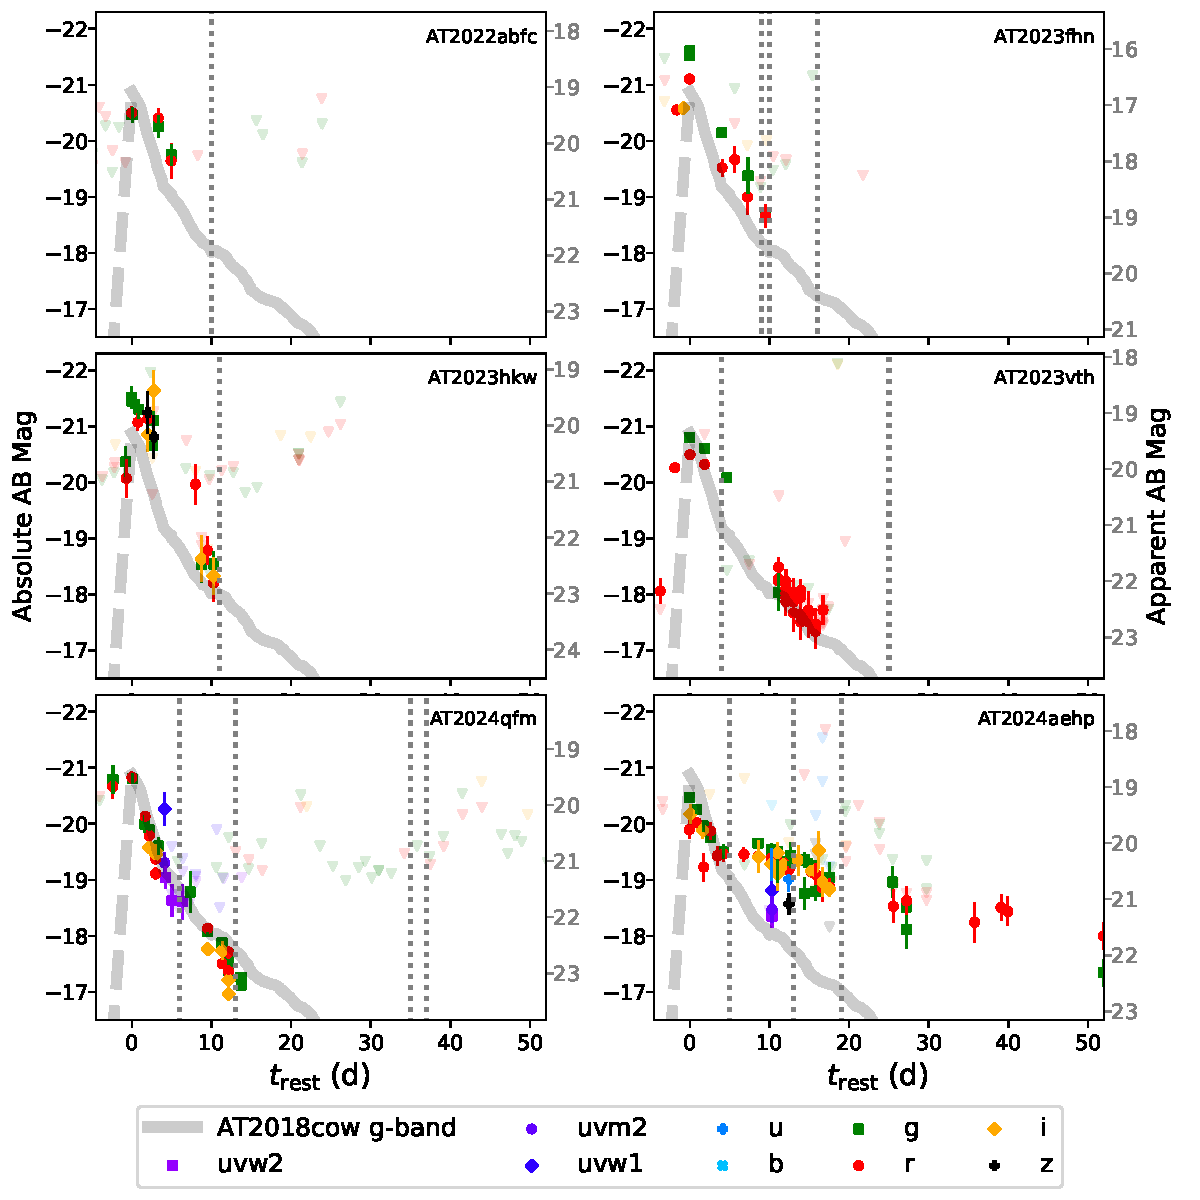
\includegraphics[width=\linewidth]{fig1_optical.pdf}
\caption{Optical light curves of each LFBOT (points), as well as the light curve of AT2018cow (thick gray line, where dashed lines mark the connection to the last upper limit).  The left-hand ordinate values display the $E(B-V)$ corrected absolute AB magnitude \citep{abmag} and are shared for all plots.  The right-hand ordinate displays the apparent AB magnitude.  Each filter has a unique marker color and style. Upside-down triangles represent 3-$\sigma$ upper limits. The vertical {\bf dotted} lines show when spectra of the transient and/or its host galaxy were taken.  These spectra are displayed in Figure~\ref{fig:spec}.}
\label{fig:optical}
\end{figure*}
 
\subsection{Optical Spectroscopy}
\label{sec:optical-spectroscopy}

As part of our follow-up campaigns, we  collected optical spectra at $t_{\text{obs}}=4$--37 days. We utilized the following facilities: the Gemini Multi-Object Spectrograph (GMOS; \citealt{gmos-n}, \citealt{gmos-s}), the Keck Low-Resolution Imaging Spectrometer (LRIS; \citealt{lris}) on the 10\,m Keck-I telescope, the Keck Cosmic Web Imager (KCWI; \citealt{kcwi}) and the Deep Imaging Multi-Object Spectrograph (DEIMOS; \citealt{deimos}) on the 10\,m Keck-II telescope, the Double Spectrograph on the Palomar 5\,m telescope (DBSP; \citealt{p200_dbsp}), and the Binospec instrument \citep{Fabricant2019} on the 6.5\,m Multiple Mirror Telescope (MMT). \added{The basic details for each spectroscopic observation are provided in Table~\ref{tab:spectra} within Appendix~\ref{sec:appendix-tables}.} 

\added{Spectra are shown in Figure~\ref{fig:spec}. In all cases narrow emission lines are observed from the LFBOT host galaxies, (e.g., \ion{Ca}{2} H\&K, [\ion{N}{2}], [\ion{O}{2}], [\ion{O}{3}], and [\ion{S}{2}]). The Balmer H$\alpha$ line is prominent for all six objects. Spectra were obtained at the position of the transient (Figure~\ref{fig:cutouts}) at a time when the transient and the host galaxy's brightness are comparable (Figure~\ref{fig:optical}) so they typically contain contributions from both the transient and its host galaxy. All narrow emission lines we identified are well-known galactic emission lines; we do not identify any clear features from the transient itself, which is unsurprising given that at these phases LFBOT spectra are dominated by a blue continuum that is well approximated by a blackbody (e.g., \citealt{margutti,perley2021}).}

\begin{figure*}[t]
 \centering
  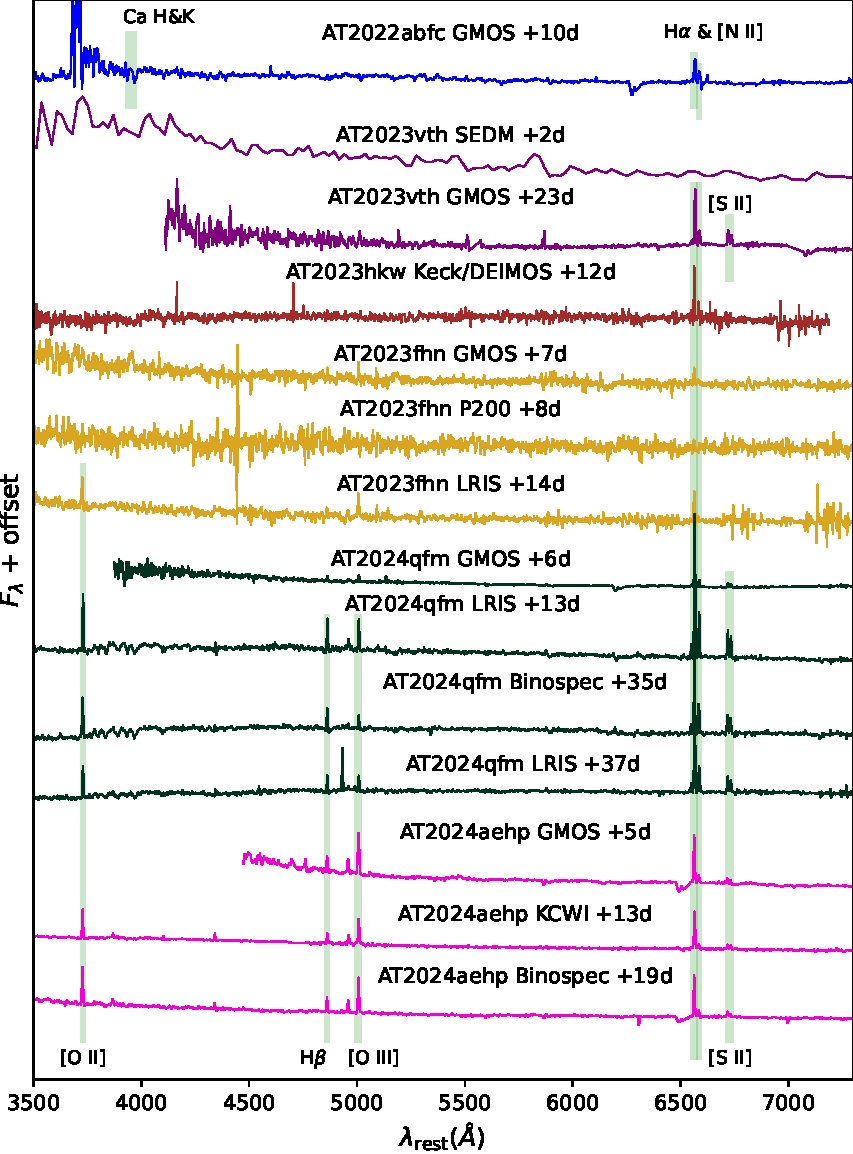
\includegraphics[width=0.85\textwidth]{fig2_spec_full.pdf}
\caption{Spectra of each LFBOT and/or its host galaxy. For each spectrum we indicate the observer-frame epoch and instrument used. {\bf We bin all spectra with a bin size of  3 \AA}.  The green shaded rectangles show  galactic narrow emission lines that were used to determine a redshift. The spectra are displayed with an arbitrary vertical offset.
}
\label{fig:spec}
\end{figure*}

\begin{figure*}[]
 \centering
  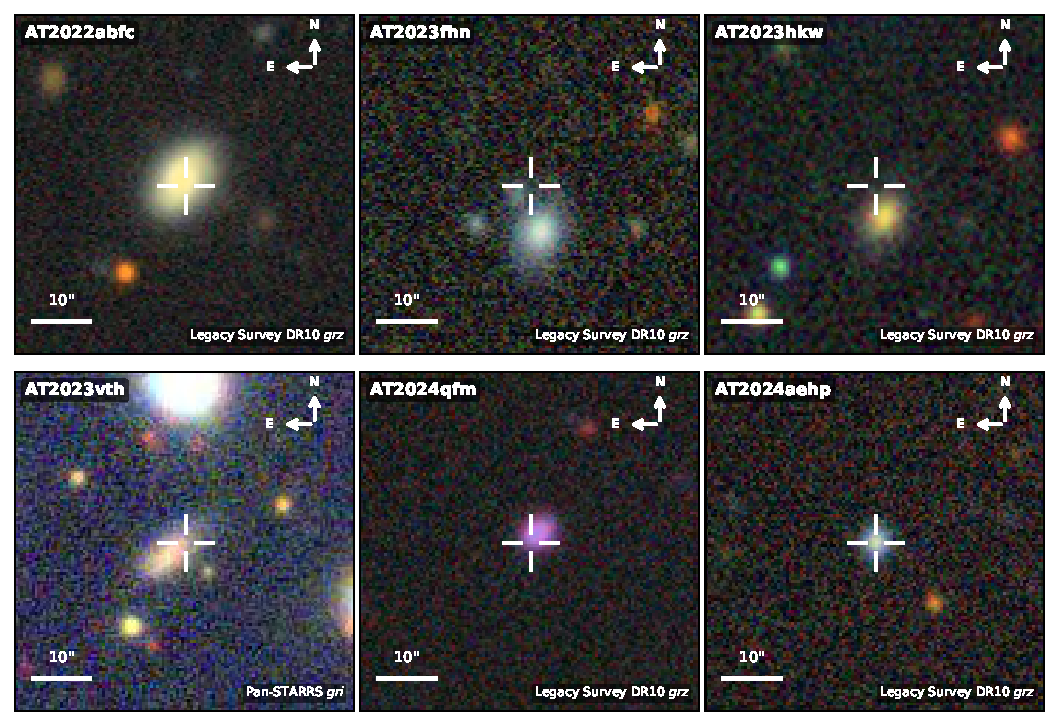
\includegraphics[width=\linewidth]{fig3_host_cutouts.pdf}
\caption{{\bf Optical cutouts of the six LFBOT host galaxies we discuss in this paper. In each panel we mark the position of the LFBOT with cross hairs.}}
\label{fig:cutouts}
\end{figure*}


\subsection{Swift X-ray Observations}

\begin{figure*}[t]
 \centering
  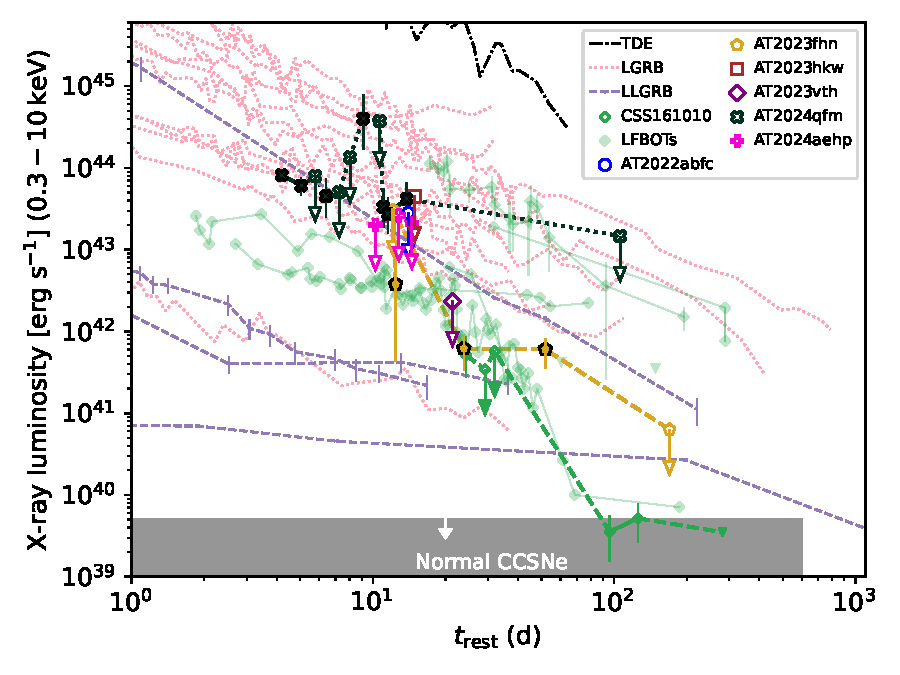
\includegraphics[width=0.7\linewidth]{fig4_x_collage.pdf}
\caption{0.3--10\,keV X-ray light curves of the six LFBOTs in this paper, in comparison to those of other LFBOTs, {\bf long gamma-ray bursts (LGRBs), and low-luminosity gamma-ray bursts (LLGRBs)}. Open symbols with downward-facing triangles mark 3-$\sigma$ upper limits.  Data are from \citet{pian2000}, \citet{tiengo2004}, \citet{campana2006b}, \citet{soderberg2006b}, \citet{blanchard2017}, \citet{ho2020blt}, \citet{coppejans2020}, \citet{hinkle2021}, \citet{perley2021},\citet{yao2022}, \citet{ho2022}, \citet{perley2023abvizsw}, \citet{ho2023tsd}, \citet{chrimes2024}, \added{\citet{yao2024}}, and \citet{Perley2026}, as well as public \swift\ data.}
\label{fig:xray}
\end{figure*}

X-ray observations were obtained with the \emph{Swift} X-ray Telescope (XRT; \citealt{swift_xrt}) \added{in the 0.3--10\,keV range} by 
%target-of-opportunity 
ToO triggers shortly after discovery of each LFBOT.  Count rates for the XRT instrument were obtained from the UKSSDC \swift\ light-curve generator\footnote{\href{https://www.swift.ac.uk/user_objects/lc_docs.php}{UKSSDC \swift\ Light-Curve Generator}}.  Utilizing tools from NASA HEASARC, we converted these count rates to an X-ray flux accounting for the \ion{H}{1} column density in the Milky Way. For upper limits (all objects except AT2024qfm), we assume a power-law photon index of $\Gamma=2$, a typical value for previous LFBOTs \citep{sandoval2018, margutti, bright2022,matthews2023}. %and also a typical value we infer in this paper.

For AT2024qfm, \swift\ obtained 12 observations, from $t_{\text{obs}}\sim8$--133\,d after the first optical detection. We visually inspected the images and discarded one observation (ID 00016748006) because the source landed on the XRT detector's hot column.  The X-ray light curve shows a general decline, with the exception of one observation 
(ID 00016748007) which showed a significant rebrightening. This observation was extremely short, with 233\,s of raw exposure but only 40\,s of clean data. Two source counts were detected at the position of AT2024qfm; using the \citet{Kraft1991} approach of the \swift\ tools, the implied detection significance is 99.83\% (just over 3-$\sigma$). Closer inspection of the data revealed no clear reason why this would be an erroneous measurement.%From the first two observations, we found a best-fit photon index of $\Gamma=2.0^{+0.6}_{-0.5}$. 
%We used $n_H=4.74\times10^{20}\,$cm$^{-2}$ \citep{Willingale2013}. The counts-to-unabsorbed-flux conversion rate was therefore $3.92\times10^{-11}$\,erg\,s$^{-1}$\,cm$^{-2}$\,ct$^{-1}$. 

For purpose of comparison and for completeness, we also analyze three early \emph{Swift} XRT observations of the LFBOT CSS161010. Late-time (100\,d) observations were presented in \citet{coppejans2020}, while upper limits for these early observations were presented in \citet{Gutierrez2024} (see their Appendix~A.1). We find a very marginal (3.3-$\sigma$) detection in the first epoch, and non detections in the subsequent two epochs. Our upper limits are within a factor \added{of three of those in \citet{Gutierrez2024}, who presented binned measurements}.  We also show the \added{0.2--10\,keV} \chandra\ measurements of AT2023fhn published by \citet{chrimesfhn}, using the revised values in \citet{nayana2025}.

The \swift\ XRT observations are summarized in Table~\ref{tab:xray} in Appendix~\ref{sec:appendix-tables}.  Five of the \added{new} LFBOTs had a \swift\ non-detection, resulting in upper limits for the photon count rate and the X-ray flux.  These upper limits are compared to other objects with \swift\ detections in Figure~\ref{fig:xray}. 
%X-ray flux of $2.6_{-1.1}^{+2.4} \times 10^{-15}$ erg cm$^{-2}$ s$^{-1}$ (0.5--7.0\,keV), corresponding to a luminosity of $1.3_{-0.3}^{+0.4}\times 10^{42}$ erg s$^{-1}$.  
%We also analyze three \swift observations of another LFBOT, CSS161010, between 24 and 32 days (observer frame) after peak light.  Only one resulted in a detection, with an X-ray flux of $1.8 _{-0.9}^{+1.4} \times 10^{-13}$ erg cm$^{-2}$ s$^{-1}$ (0.3-10 keV), which corresponds to a luminosity of $4.8^{+3.6}_{-2.4}\times 10^{42}$ erg s$^{-1}$.

\subsection{Radio and Millimeter Observations}

 We obtained radio observations with the National Science Foundation's Karl G. Jansky Very Large Array (VLA; \citealt{vla, evla}), the Giant Metrewave Radio Telescope (GMRT; \citealt{gmrt}), and the Northern Extended Millimeter Array (NOEMA).  All of these observations are listed in Table~\ref{tab:radio} in Appendix~\ref{sec:appendix-tables}.
 
\subsubsection{VLA}

We present VLA observations for five LFBOTs\footnote{AT2022abfc was observed under programs 22A-405 (PI D. Perley), 23A-393, 23A-422, and 23B-138;  AT2023fhn under programs 23A-403 and 23B-138;  AT2023vth under program 23B-138;  AT2023hkw under program 23A-415; AT2024aehp under programs 24B-338 and 25A-367 (PI A. Ho)}, all of which were detected. Radio data for AT2024qfm will be published by Nayana A.J. et al. in prep \added{as per a prior arrangement}. Observations were obtained at mid-frequencies of 3 GHz (S-band), 6 GHz (C-band), 10 GHz (X-band), 16 GHz (Ku-band), and 33 GHz (Ka-band).
Based on the behavior of past sources \added{\citep{yao2022, ho2022xnd, chrimes2024}}, 10 GHz (X-band) gives the most reliable chances of detection, so every epoch features an observation in this band. We calibrate VLA data using the automated pipeline in Common Astronomy Software Applications package version 6.5.4-9 (CASA; \citealt{casa}).   We use Briggs weighting with \texttt{robust = 0.5} \citep{briggs1995}.  When the image quality is degraded by bright artifacts from nearby luminous sources, we perform phase-only self-calibration on these other sources. Flux measurements were determined by using the Cube Analysis and Rendering Tool (CARTA; \citealt{carta}). For detections, the flux density is the maximum intensity at the transient's position, and the uncertainty is the measured root-mean square (RMS) in the background. For non-detections, we take the upper limit to be 3 $\times$ RMS. The radio light curves are shown in Figure~\ref{fig:radio-lc} and the radio SED evolution is shown in Figure~\ref{fig:radio-sed}.

\begin{figure}[!h]
 \centering
  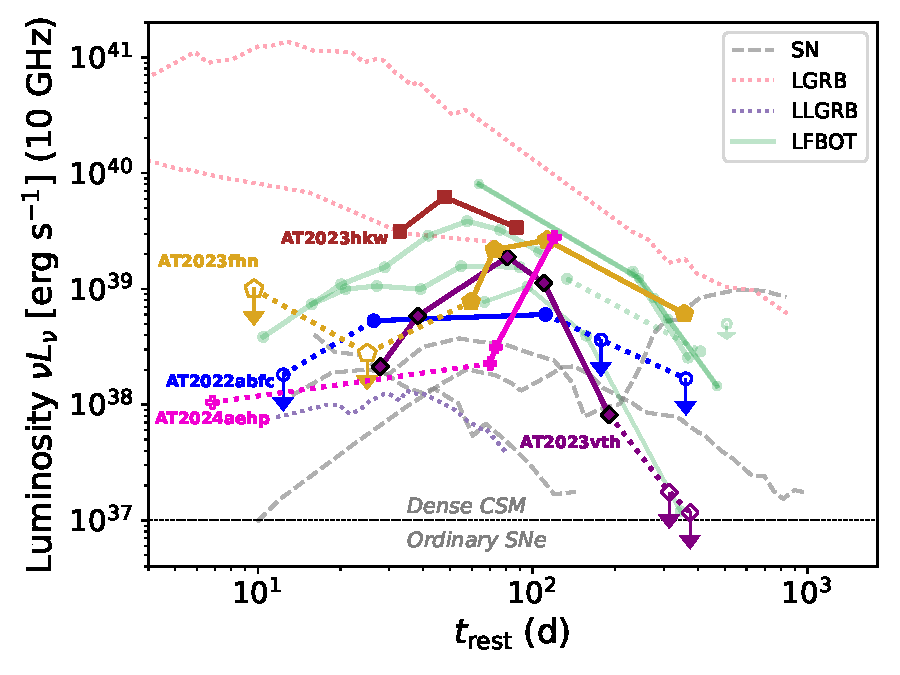
\includegraphics[width=\linewidth]{fig5_radio_collage.pdf}
\caption{Radio light curves at 10 GHz of the LFBOTs with data presented in this paper, compared with other known LFBOTs, long GRBs (LGRBs), low-luminosity GRBs (LLGRBs), and core-collapse supernovae with non-relativistic ejecta (SNe). We measure time after peak light in the transient's rest frame.  Data from \citet{1998bwradio}, \citet{berger2003}, \citet{soderberg2006}, \citet{vanderhorst2008}, \citet{soderberg2010}, \citet{salas2013}, \citet{margutti}, \citet{coppejans2020}, \citet{ho2022xnd}, \citet{yao2022}, \citet{perley2021}, \citet{ho2023tsd}, and \citet{nayana2025}.}
\label{fig:radio-lc}
\end{figure}

\begin{figure*}[]
 \centering
  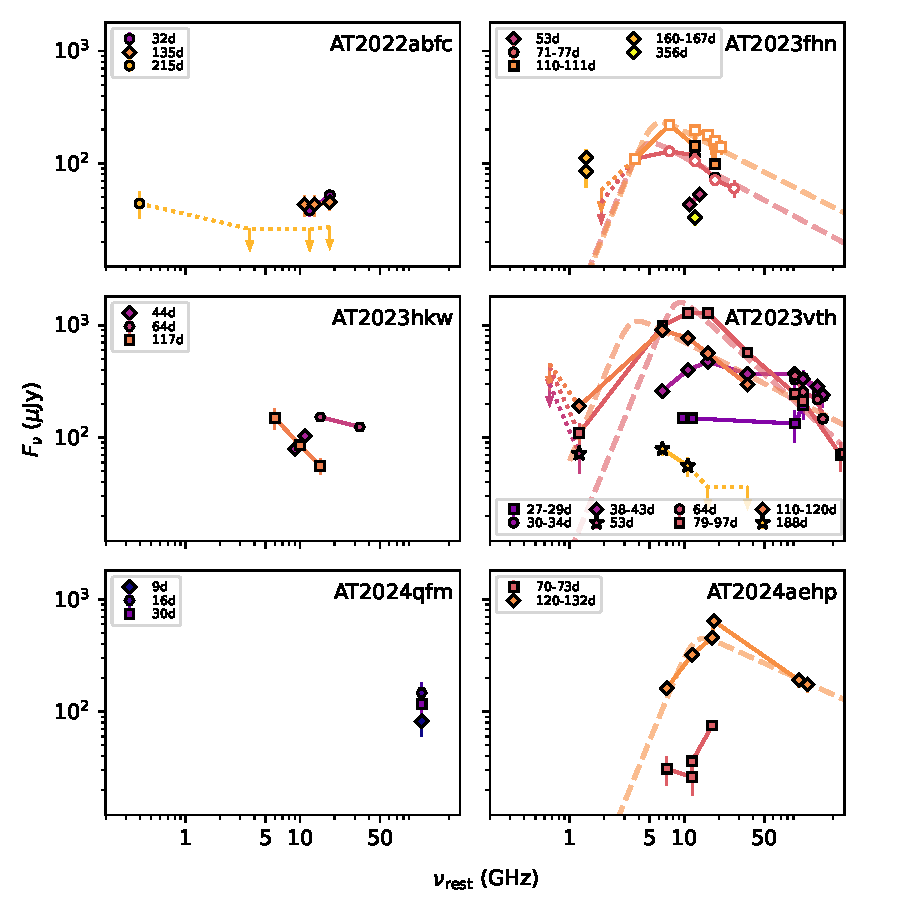
\includegraphics[width=\linewidth]{fig6_radio_sed.pdf}
\caption{The radio and millimeter SED of each LFBOT at different observer-frame epochs.  Observations taken within a few days are grouped into one epoch.  Non-detections are signified by {\bf a downward pointing arrow}.  For clarity, we omit some non-detections.  For epochs with sufficient data points, we display the broken power-law fit to the SED as a dashed line.  Data from \citet{chrimes2024} for AT2023fhn {\bf have markers filled in with white.}}
\label{fig:radio-sed}
\end{figure*}

\subsubsection{GMRT}
We also present GMRT observations of  AT2022abfc, AT2023fhn, AT2023hkw, and AT2023vth. Both AT2023fhn and AT2023vth were detected. These observations were spread across three frequency bands: Band-3 (250-500 MHz), Band-4 (550-850 MHz), and Band-5 (1000-1460 MHz)\footnote{AT2022abfc was observed under program ID 44\_099.  AT2023fhn was observed under programs 45\_117 and ddtC299.  AT2023hkw was observed under 45\_117 and ddtC294.  AT2023vth was observed under program 45\_113 (PI Nayana A.J.).}.
The GMRT data were reduced through CASA and AIPS.  We use Briggs weighting with \texttt{robust = 0.5}.  The primary beam correction was done following the method described in the CASA documentation\footnote{\href{https://casadocs.readthedocs.io/en/latest/examples/community/Example_Wideband_PrimaryBeamCorrection.html\#Imaging-With-Custom-Primary-Beams}{CASA: Imaging with Custom Primary Beams}}.  We measure the flux density using the \texttt{imfit} method in the CASA documentation, which provides the maximum intensity for a fitted Gaussian.  If the measured flux is not 3-$\sigma$ above the background flux RMS, we record an upper limit of 3$\times\,$the RMS. 

\subsubsection{NOEMA}

We observed five LFBOTs using NOEMA\footnote{Program IDs W22BT (AT2023fhn and AT2022abfc), W24EW (AT2024aehp), S23BF (AT2023vth), D24AA (Director's Discretionary Time; AT2024qfm), all PI A. Ho.} (all but AT2023hkw), at times ranging from $t=10$--100\,d, resulting in detections of three objects (AT2024aehp, AT2024qfm, AT2023vth) and non-detections of two objects (AT2022abfc, AT2023fhn). The data reduction was done with Continuum and Line Interferometer Calibration (\texttt{CLIC}) and \texttt{MAPPING}, which are part of the \texttt{GILDAS} software package \citep{gildas}\footnote{\href{https://www.iram.fr/IRAMFR/GILDAS}{https://www.iram.fr/IRAMFR/GILDAS}}. Unless otherwise specified, all uncertainties are 1$\sigma$, and \added{the systematic error of the} flux scale is 10\% in the 3\,mm band and 15\% at 1.3\,mm. The NOEMA data are provided in Table~\ref{tab:radio} and displayed in Figure~\ref{fig:mm}. 

AT2024aehp was observed on May 23, 2025 ($>100\,$d after optical discovery; we triggered mm observations following the cm-wave detection) in the 10D configuration under mediocre weather conditions, with MWC349 as the flux calibrator. Reduction was performed by hand and we estimate a 15\% systematic calibration uncertainty for the absolute flux scale. 

AT2023fhn was observed on April 22, 2023 in the 12C configuration under good conditions, with LKHA101 as the flux calibrator. The image included a nearby bright source, and subtracting the contribution from the bright source did not result in a detection of AT2023fhn at the phase center. 

An observation of AT2022abfc was triggered on December 30, 2022; an attempt was made on January 7, 2023, but could not be carried out owing to bad weather. A successful observation was obtained on January 10 in the 12A configuration, with LKAH101 as the flux calibrator. The source was not detected, but limits were weak because the source was at high airmass and the array was in an extended configuration.

AT2023vth was first observed on November 20, 2023 in the 9C configuration, under cloudy conditions, with the flux calibrator MWC349. The source was detected, so we pursued multifrequency follow-up observations. The timing of these observations was affected by weather conditions, particularly at the highest frequencies. 

NOEMA observed AT2024qfm on four
dates, in compact configuration (D), with primary flux calibrator MWC349. The first observation was on August 5, 2024. The source was detected in the first three epochs. %For AT2023vth, we display the results for a rest frequency of 100 GHz.
%In these regime, the LFBOTs we study display considerable variation.  
%NOEMA observations at 100 GHz are displayed in Figure~\ref{fig:mm}.

\begin{figure}[!h]
 \centering
  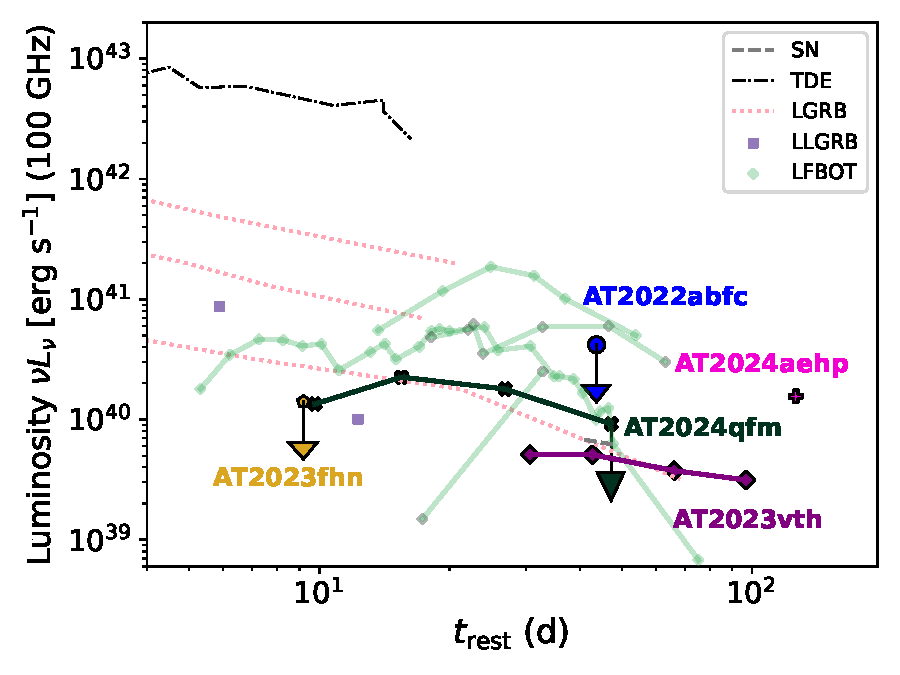
\includegraphics[width=\linewidth]{fig7_mm_collage.pdf}
\caption{Millimeter-wave (100\,GHz) light curves in comparison to other LFBOTs, long-duration gamma-ray bursts (LGRBs), low-luminosity GRBs (LLGRBs), and tidal disruption events (TDEs).  AT2022abfc and AT2023fhn only have an upper limit. AT2023fhn has been shifted slightly to the left for clarity. Data are from \citet{1998bwradio, zauderer2011, perley2013_130427a, corsi2014, laskar2016, perley2017_171205a, laskar2018, margutti, bright2022, ho2023tsd, nayana2025}.}
\label{fig:mm}
\end{figure}

\subsection{Search for Gamma-Ray Bursts}
We performed an archival search for GRB detections in the  NASA General Coordinates Network Circulars\footnote{\href{https://gcn.nasa.gov/circulars/}{https://gcn.nasa.gov/circulars/}}.  We looked for GRBs detected within a week of the transient's optical light-curve peak \added{that had a localization that was within 3-$\sigma$ of the transient's coordinates}. No such GRBs were reported.
\newline
\newline
\subsection{Search for X-ray Precursors}

\added{One way to distinguish between LFBOT progenitor models could be to detect precursor emission: this might be expected in a model with runaway mass transfer leading up to the dynamical merger of a stripped star and compact-object companion \citep{metzger2022,Tsuna2024} but not in e.g., a core collapse scenario.} We searched for X-ray precursor emission in the eROSITA-DE Data Release 1 (DR1). eROSITA \citep{eROSITA} is the soft X-ray instrument onboard the orbital observatory Spectrum-Roentgen-Gamma (SRG; \citealt{SRG2021}). DR1 comprises data from the first six months, which ended in June 2020 \citep{Merloni2024,TubinArenas2024}.  

Of the thirteen LFBOTs in Table~\ref{tab:summary}, three were in the footprint of eROSITA-DE DR1: AT2022abfc, CSS161010, and AT2024wpp. For each object, we used the products from \citet{TubinArenas2024} and \citet{Merloni2024} to determine if there was a detection at the source position, and if not, obtained a 0.2--2.3\,keV upper limit (the most sensitive energy range for eROSITA).  \added{As each field was only imaged once in this data release, we only check for consistency in position and allow the observation to be at any time.}  The closest catalogued sources were \added{offset by} $5.5^{\prime}$ (AT2022abfc), $3^{\prime}$ (CSS161010), and $2^{\prime}$ (AT2024wpp), too distant to be associated \added{(the spatial resolution of eROSITA is $<10^{\prime\prime}$, \citealt{eROSITA})}.

For AT2022abfc and AT2024wpp (the two objects for which the eROSITA observations were prior to the LFBOT), the limits are $9.1\times10^{42}$\,erg\,s$^{-1}$ corresponding to 2.7\,yrs pre-LFBOT, and $9.0\times10^{41}$\,erg\,s$^{-1}$ corresponding to 4.7\,yrs pre-LFBOT, respectively. For CSS161010, the eROSITA limit is $1.5\times10^{41}$\,erg\,s$^{-1}$, 3.4\,yrs after the LFBOT. The next eROSITA data release (scheduled for mid-2026) will provide more stringent upper limits (i.e., closer to the LFBOT time).  

\subsection{Host-Galaxy Photometry}
%We also obtained photometry for each LFBOTs host galaxy%, and the offset between the LFBOT and its host. To get the LFBOT host positions, we used the Legacy Survey Data Release 10 for AT2022abfc, the Sloan Digital Sky Survey \citep{sdss} for AT2023hkw, Pan-Starrs1 \citep{panstarrs} for AT2023vth, and \citet{chrimesfhn} for AT2023fhn. 
IR and UV photometry were obtained for all LFBOT host galaxies from the Near-Earth Object Wide-field Infrared Survey Explorer mission (NEOWISE; \citealt{neowise}) on the {\em Wide-field Infrared Survey Explorer} space telescope (\wise), and the {\em Galaxy Evolution Explorer} (\galex; \citealt{galex}), respectively.  Optical photometry for the host galaxies was obtained from the Legacy Survey Data Release 10 \citep{legacy}. The host galaxy of AT2023vth does not have Legacy Survey optical photometry, so we used optical photometry from Pan-STARRS DR2 (PS1; \citealt{panstarrs}).  We also used {\it Hubble Space Telescope (HST)} photometry from \citet{chrimesfhn} for AT2023fhn.  All the {\galex} data used in this paper can be found in MAST: \dataset[10.17909/zktz-mn64]{http://dx.doi.org/10.17909/zktz-mn64}.  For the photometry in all bands, we required a signal-to-noise ratio (SNR) greater than 5 for a detection.  \added{We choose this SNR to include several marginal {\bf GALEX} and {\bf WISE} detections, while excluding a few measurements with errors of over 0.5 mag.  Choosing a stricter cutoff would make the fit far more uncertain as we lose a significant number of data points, but a looser cutoff would have little effect as the new points would have large errors, which the fitting process accounts for.  We display cutouts of the host galaxies in Figure~\ref{fig:cutouts}. }

We used the Python package \texttt{gPhoton} \citep{gphoton} to retrieve \galex\ near-UV and far-UV photometry for the LFBOT host galaxies.  In \texttt{gPhoton}, we chose the observation with the longest exposure time and recorded the background-corrected magnitudes.  We chose an aperture radius of 6.12 arcseconds for the source, and measured the background from an annulus with an inner radius of 10.8 arcseconds and an outer radius of 21.6 arcseconds.  \added{We estimate that this size would exclude all of the host galaxy's emission and include as much background as possible for an accurate background flux estimate without including any flux from other sources.  We apply this annulus size to most of the LFBOT hosts to maintain consistency.}  In the cases of AT2023hkw and AT2023vth, there were \added{nearby UV-bright sources that required us to use a smaller annulus}.  The inner and outer annulus radii are 10.8 and 16.2 arcseconds for AT2023hkw, and 7.2 and 10.8 arcseconds for AT2023vth.  Legacy Survey and {\it NEOWISE} photometry was obtained with the Python package \texttt{noaodatalab}\footnote{\href{https://github.com/astro-datalab/datalab}{https://github.com/astro-datalab/datalab}} version 2.20.0.  Pan-STARRS DR2 {\em grizy} photometry was \added{retrieved through} the online catalog search tool\footnote{\href{https://catalogs.mast.stsci.edu/panstarrs/}{https://catalogs.mast.stsci.edu/panstarrs/}}.

The host-galaxy photometry is provided in Table~\ref{tab:galaxy} in Appendix~\ref{sec:appendix-tables}.



 %This similarity suggests that the source of the radio emission (synchrotron radiation from the transient's shock) is a crucial factoring in determining whether a transient will be an AT2018cow-like FBOT.


%AT2023fhn is less luminous in the millimeter band than other detected LFBOTs by 1--2 orders of magnitude. %, and far less than that of TDEs and GRBs.  
%While we also have a non-detection for AT2022abfc, the poor observing conditions means that we cannot rule out AT2018cow-emission for this transient.  For AT2023vth, we detect the mm-wave emission out to 100 days after peak light. 

\section{Radio Analysis}
\label{sec:radio-analysis}

\subsection{Radio Synchrotron Modeling}
\label{sec:synchro}

We model the SED
at radio and millimeter wavelengths as the result of synchrotron emission.  Synchrotron radiation with a self-absorbed component forms a broken power-law radio SED. We follow the prescription of \citet{chevalier} to derive properties of the shock and the medium it traverses, such as the shock radius, ambient magnetic field, average shock velocity, pre-shock density, and total shock energy.  This is the same procedure used in modeling the radio SEDs for other AT2018cow-like FBOTs (e.g., \citealt{margutti,ho2019,chrimesfhn,nayana2025,Perley2026}). We note that in some of these works, some equations are given in terms of angular diameter distance $D_\theta$, but should be given in terms of luminosity distance ($D_L$; private communication) as in the expressions below. 
\added{We also note that the following prescription assumes a nonrelativistic shock and does not account for relativistic effects (see, e.g., \citealt{margalit2024, ferguson2025}), which become relevant for $\Gamma \beta \sim1$. 
For self-consistency, we estimate the $\Gamma \beta$ this model outputs and we find that some objects do approach the trans-relativistic regime (Fig~\ref{fig:synchrotron}), so we caution against taking our presented results at face value for the higher-velocity events. Still, we use this method for comparison with previous LFBOTs, which is the main goal of this paper's analysis.} 

As in \citet{soderberg2010b}, we assume equipartition of energy between protons, electrons, and the magnetic field;  thus, the energy densities in electrons ($\epsilon_e$) and magnetic fields ($\epsilon_B$) are given by $\epsilon_e=\epsilon_B=1/3$.  If we model the source of the emission as a disk with radius $R$ and thickness $S$, then its total volume is $\pi R^2 S$.  We then parameterize this as equivalent to a spherical volume $4\pi f R^3/3$, where $f$ is the filling factor.  We take $f=0.5$ as in previous LFBOT studies \citep{yao2022, bright2022}, but the dependences of the equations on this parameter is weak. We assume an electron power-law index of 3, following \citet{chevalier2006}; this is a typical value for previous LFBOTs \added{as determined from fits to the slope of the self-absorbed end of the synchrotron SED \citep{coppejans2020, ho2019}.  We do not have more than two points in the self-absorbed regime for most of our SEDs, so we use this fiducial value with the recognition that the results do not strongly depend on the optically thin power-law index \citep{chevalier}.}

Finally, we verify that the self-absorption frequency is less than the cooling frequency, which is defined as the frequency where the electrons have lost an amount of energy equal to their total energy through synchrotron cooling. We use Equation~(C13) of \citet{ho2022xnd}, which gives the ratio between the self-absorption and cooling frequencies, and confirm that the self-absorption frequency is lower for all cases.

Under these assumptions, Equations (13) and (14) from \citet{chevalier} reduce to these expressions for the shock radius and magnetic field:
\begin{equation}
\begin{split}
    R_p =& \,8.8 \times 10^{15}
    \left( \frac{\epsilon_e}{\epsilon_B}\right)^{-1/19}
    \left( \frac{f}{0.5}\right)^{-1/19}
    \left( \frac{F_{\rm p}}{(1+z)\, \text{Jy}}\right)^{9/19} \\
    &\times
    \left( \frac{D_L}{\text{Mpc}}\right)^{18/19}
    \left( \frac{\nu_{\rm p}}{5 \,\text{GHz}}\right)^{-1} \mathrm{cm}\, ,
\end{split}
\end{equation}


\begin{equation}
\begin{split}
    B =& \,0.58
    \left( \frac{\epsilon_e}{\epsilon_B}\right)^{-4/19}
    \left( \frac{f}{0.5}\right)^{-4/19}
    \left( \frac{F_{\rm p}}{(1+z)\,\text{Jy}}\right)^{-2/19} \\
    &\times
    \left( \frac{D_L}{\text{Mpc}}\right)^{-4/19}
    \left( \frac{\nu_{\rm p}}{5 \,\text{GHz}}\right) \mathrm{G}\, ,
\end{split}
\end{equation}
where $D_L$ is the luminosity distance, $\nu_{\rm p}$ \added{and $F_{\rm p}$  are the peak frequency and flux density at peak frequency of the radio SED in the transient's rest frame, respectively.}

Following \citet{ho2019}, this can then be combined into an equation for total energy $U=U_B/\epsilon_B$:

\begin{equation}
\begin{split}
    U =& \, \frac{B^2}{8\pi}\frac{4 \pi f R^3}{3}\frac{1}{\epsilon_B}\\
    =& \,1.9\times10^{46} \left( \frac{1}{\epsilon_B} \right)
    \left( \frac{\epsilon_e}{\epsilon_B}\right)^{-11/19}
    \left( \frac{f}{0.5}\right)^{8/19}\\
    &\times
    \left( \frac{F_{\rm p}}{(1+z)\,\text{Jy}}\right)^{23/19} 
    \left( \frac{D_L}{\text{Mpc}}\right)^{46/19}
    \left( \frac{\nu_{\rm p}}{5 \,\text{GHz}}\right)^{-1} \mathrm{erg}\, .
\end{split}
\label{eq:energy}
\end{equation}

We estimate the average velocity as $R/( t_{\mathrm{obs}}/(1+z))=R/ t_{\mathrm{rest}}=\Gamma \beta c$, where $\beta=v/c$ and $\Gamma$ is the Lorentz factor.

Following \citet{chrimesfhn}, we derive formulas for the CSM electron number density $n_e$ and the wind density $\dot M/v_w$.  This assumes the CSM resulted from a spherical stellar wind with mass-loss rate $\dot M$ and wind velocity $v_w$, where $\dot M/v_w=4 \pi m_p R^2 n_e$ and $m_p$ is the proton mass. Thus,

\begin{equation}
\begin{split}
    n_e =& \,1.02%418 
    \frac{1}{\epsilon_B}
    \left( \frac{\epsilon_e}{\epsilon_B}\right)^{-6/19}
    \left( \frac{f}{0.5}\right)^{-6/19}
    \left( \frac{F_{\rm p}}{(1+z)\,\text{Jy}}\right)^{-22/19} \\
    &\times
    \left( \frac{D_L}{\text{Mpc}}\right)^{-44/19}
    \left( \frac{\nu_{\rm p}}{5 \,\rm GHz}\right)^{4} 
    \left( \frac{t_{\text{rest}}}{\text{days}}\right)^{2} \mathrm{cm}^{-3}\, ,
\end{split}
\end{equation}

\begin{equation}
\begin{split}
    \frac{\dot M}{v_w}\left( \frac{1000\,\mathrm{km}\,\mathrm{s}^{-1}}{10^{-4}\,M_{\odot}\,\mathrm{yr}^{-1}}\right) =& \,2.5\times10^{-5} \left(\frac{1}{\epsilon_B}\right)
    \left( \frac{\epsilon_e}{\epsilon_B}\right)^{-8/19} \\
    &\times \left( \frac{f}{0.5}\right)^{-8/19}
    \left( \frac{F_{\rm p}}{(1+z)\,\text{Jy}}\right)^{-4/19} \\
    &\times
    \left( \frac{D_L}{\text{Mpc}}\right)^{-8/19}
    \left( \frac{\nu_{\rm p}}{5 \,\text{GHz}}\right)^{2} \\
    &\times \left( \frac{t_{\text{rest}}}{\text{days}}\right)^{2}\, .
\end{split}
\end{equation}

The peak frequency and flux density of the SED at a given epoch are measured by fitting a smoothed broken-power law of the form
\begin{equation}
F(\nu)=F_{\rm p}\left((\nu/\nu_{\rm p})^{-sa_1}+(\nu/\nu_{\rm p})^{-sa_2}\right)^{-1/s}.
\label{eq:broken}
\end{equation}

We choose $s=1$ for the smoothness parameter, as was done in previous LFBOT studies \citep{bright2022, chrimes2024, nayana2025}.  We also set $a_1=5/2$ to fix the power-law slope of the self-absorbed half of the SED, as required by Chevalier's formulation. When an epoch involves observations from multiple \added{observatories}, \added{we apply an extra error in quadrature equal to 10\% of the flux density to account for systematic effects between arrays}.  A fit is performed only when we have detections on either side of the SED's peak.  The best-fit parameters from the broken power-law fit are provided in Table~\ref{tab:synchro_fit} in Appendix~\ref{sec:appendix-tables}.  If we are unable to perform a broken power-law fit, we use the values at the detection closest to the peak's implied location in place of the frequency and flux density at peak, and calculations based on these values will instead set limits on the synchrotron parameters.  
The inferred synchrotron parameters are listed in Table~\ref{tab:synchro} in Appendix~\ref{sec:appendix-tables}, and the results are displayed in Figure~\ref{fig:synchrotron}.  This includes epochs where we do fit a broken-power law and have point estimates for parameters, and epochs where we can only constrain the peak's location and place limits on parameters instead.  We find that the implied CSM densities for these six LFBOTs are comparable to those derived in the literature for previous LFBOTs, with values of 10--100 $\mathrm{cm}^{-3}$ at radii of $10^{17} \mathrm{cm}$.  
%$\dot{M}\approx10^{-4}\,M_{\odot}\,\mathrm{yr}^{-1}$ assuming a wind velocity of 1000\, km s$^{-1}$.  %Owing to AT2024aehp's unusual radio evolution (late brightening), we caution against taking these results at face value for this LFBOT.

\begin{figure*}[!htb]
 \centering
  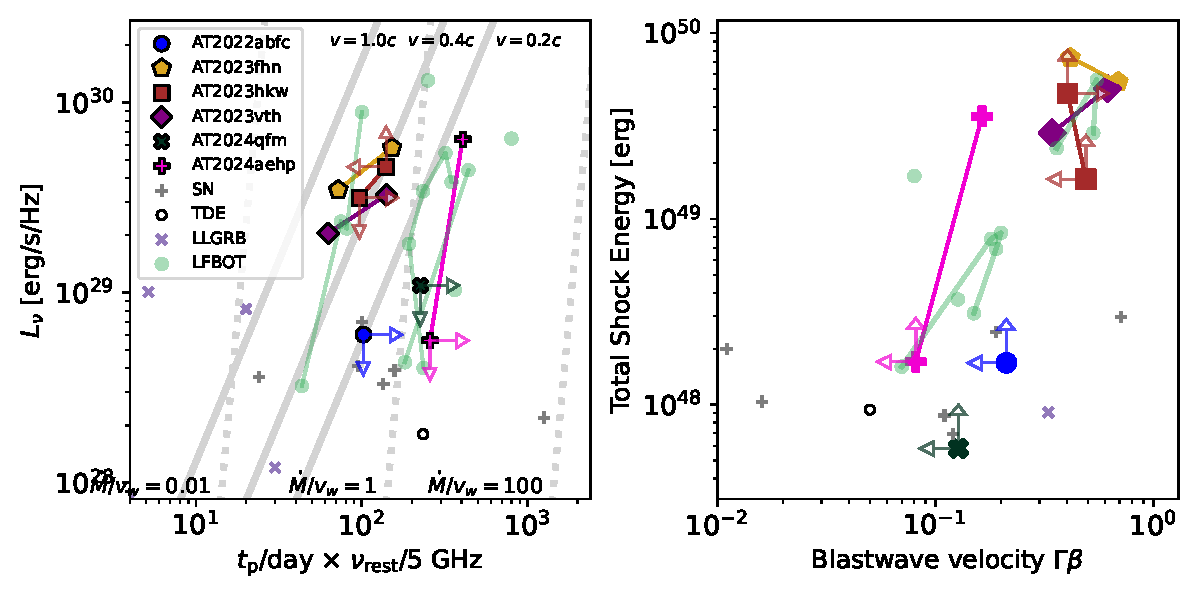
\includegraphics[width=\linewidth]{fig8_synchrotron.pdf}
\caption{Inferred parameters from our synchrotron self-absorption modeling.  Some epochs do not include the self-absorption peak and merely constrain its location; the corresponding upper limits on parameters are marked with arrows. Values for other objects are obtained from \citet{ho2019} and \citet{ho2023tsd}; and \citet{Perley2026} for AT2024wpp.  We label each object and the observer-frame time after peak light. \emph{Left:} Luminosity density at $\nu_p$ versus peak frequency and time after explosion.  We also display lines of constant shock velocity and $\dot{M}/v_w$, where $v_w=1000$\,km s$^{-2}$ and $\dot{M}$ is in units of $10^{-4}\,M_{\odot}\,\mathrm{yr}^{-1}$. \emph{Right}: Total shock energy derived from Equation~\ref{eq:energy} against shock velocity in terms of $\Gamma \beta$.  }
\label{fig:synchrotron}
\end{figure*}

\section{Host-Galaxy Analysis}
\label{sec:host-analysis}

\subsection{Host-Galaxy Offsets}\label{sec:offset}
\added{With an expanded sample of 13 LFBOTs (double the previous size in the literature), we also examine the distribution of LFBOT offsets from the host-galaxy nuclei.  We choose the host galaxy as the galaxy closest in offset to the transient, and then confirm that there are no lines at conflicting redshifts in spectroscopy of the LFBOT and its host.  To measure offsets, we require accurate localizations of each LFBOT and its host galaxy.}  For AT2023fhn \added{and its host}, we used the localization from {\it HST} imaging presented by \citet{chrimesfhn}.  \added{For the other LFBOTs,} we measure the host galaxy's position from Legacy Survey Data Release 10, \added{and the transient's position from a Gaussian fit in the image of the LFBOT's brightest radio detection. We also do this for AT2020xnd, which did not have a published offset.  The exceptions are} AT2023vth's host (which was measured from \added{the} Pan-STARRS Data Release 2), \added{and AT2024qfm's localization which we measure from the ZTF data (as we do not present AT2024qfm's radio data in this paper).}  These offsets are recorded in Table~\ref{tab:summary}. 

In Figure~\ref{fig:offset}, we display the cumulative distribution of all LFBOT offsets in kpc compared with other classes of extragalactic explosive transients. The offset distribution appears to be intermediate to that of CCSNe and that of LGRBs and SLSNe.  %\added{While our sample doubles the number of objects available in the literature for this kind of analysis, statistical comparisons will require 
%While the LFBOT sample size is still small, it is almost double that of previous analyses, giving us greater confidence in our results}.

%The distribution appears to be intermediate to SLSNe and CCSNe, although the number of objects is still small.


%The Figure~shows that LFBOTs tend to be closer to the galaxy's center compared to other classes of explosive transients.  While Tidal Disruption Events (TDEs) are not shown in this figure, off-nuclear TDEs more than 1 kpc from the host's center are rare \citep{yao2025}, compared to almost 80\% of LFBOTs.  

\begin{figure}[!h]
 \centering
  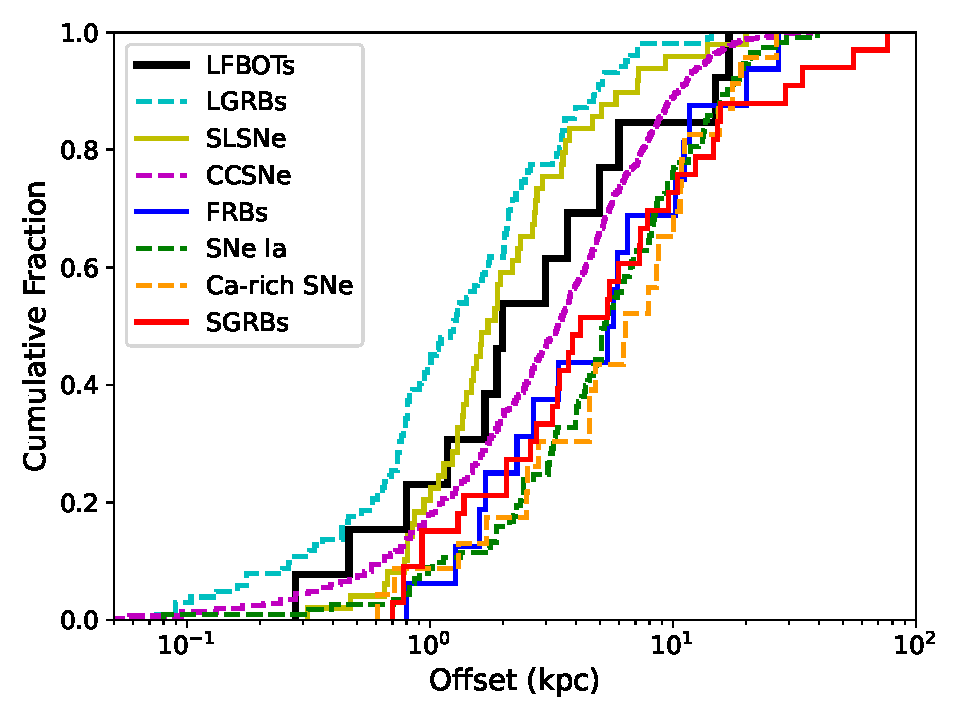
\includegraphics[width=\linewidth]{fig9_host_offset.pdf}
\caption{The cumulative distribution of host-galaxy offsets for LFBOTs, as well as fast radio bursts (FRBs; \citealt{bhandari2022}), LGRBs  \citep{blanchard2016, lyman2017}, short GRBs (SGRBs; \citealt{fong2022}), CCSNe \citep{kelly2012, schulze2021}, Type Ia SNe \citep{wang2013}, SLSNe \citep{lunnan2015, schulze2021}, and Ca-rich transients \citep{de2020}.  The offsets for previous LFBOTs are from \citet{prentice2018, coppejans2020, ho2020koala, yao2022, chrimesfhn}.}
\label{fig:offset}
\end{figure}


\begin{figure*}[!tb]
 \centering
  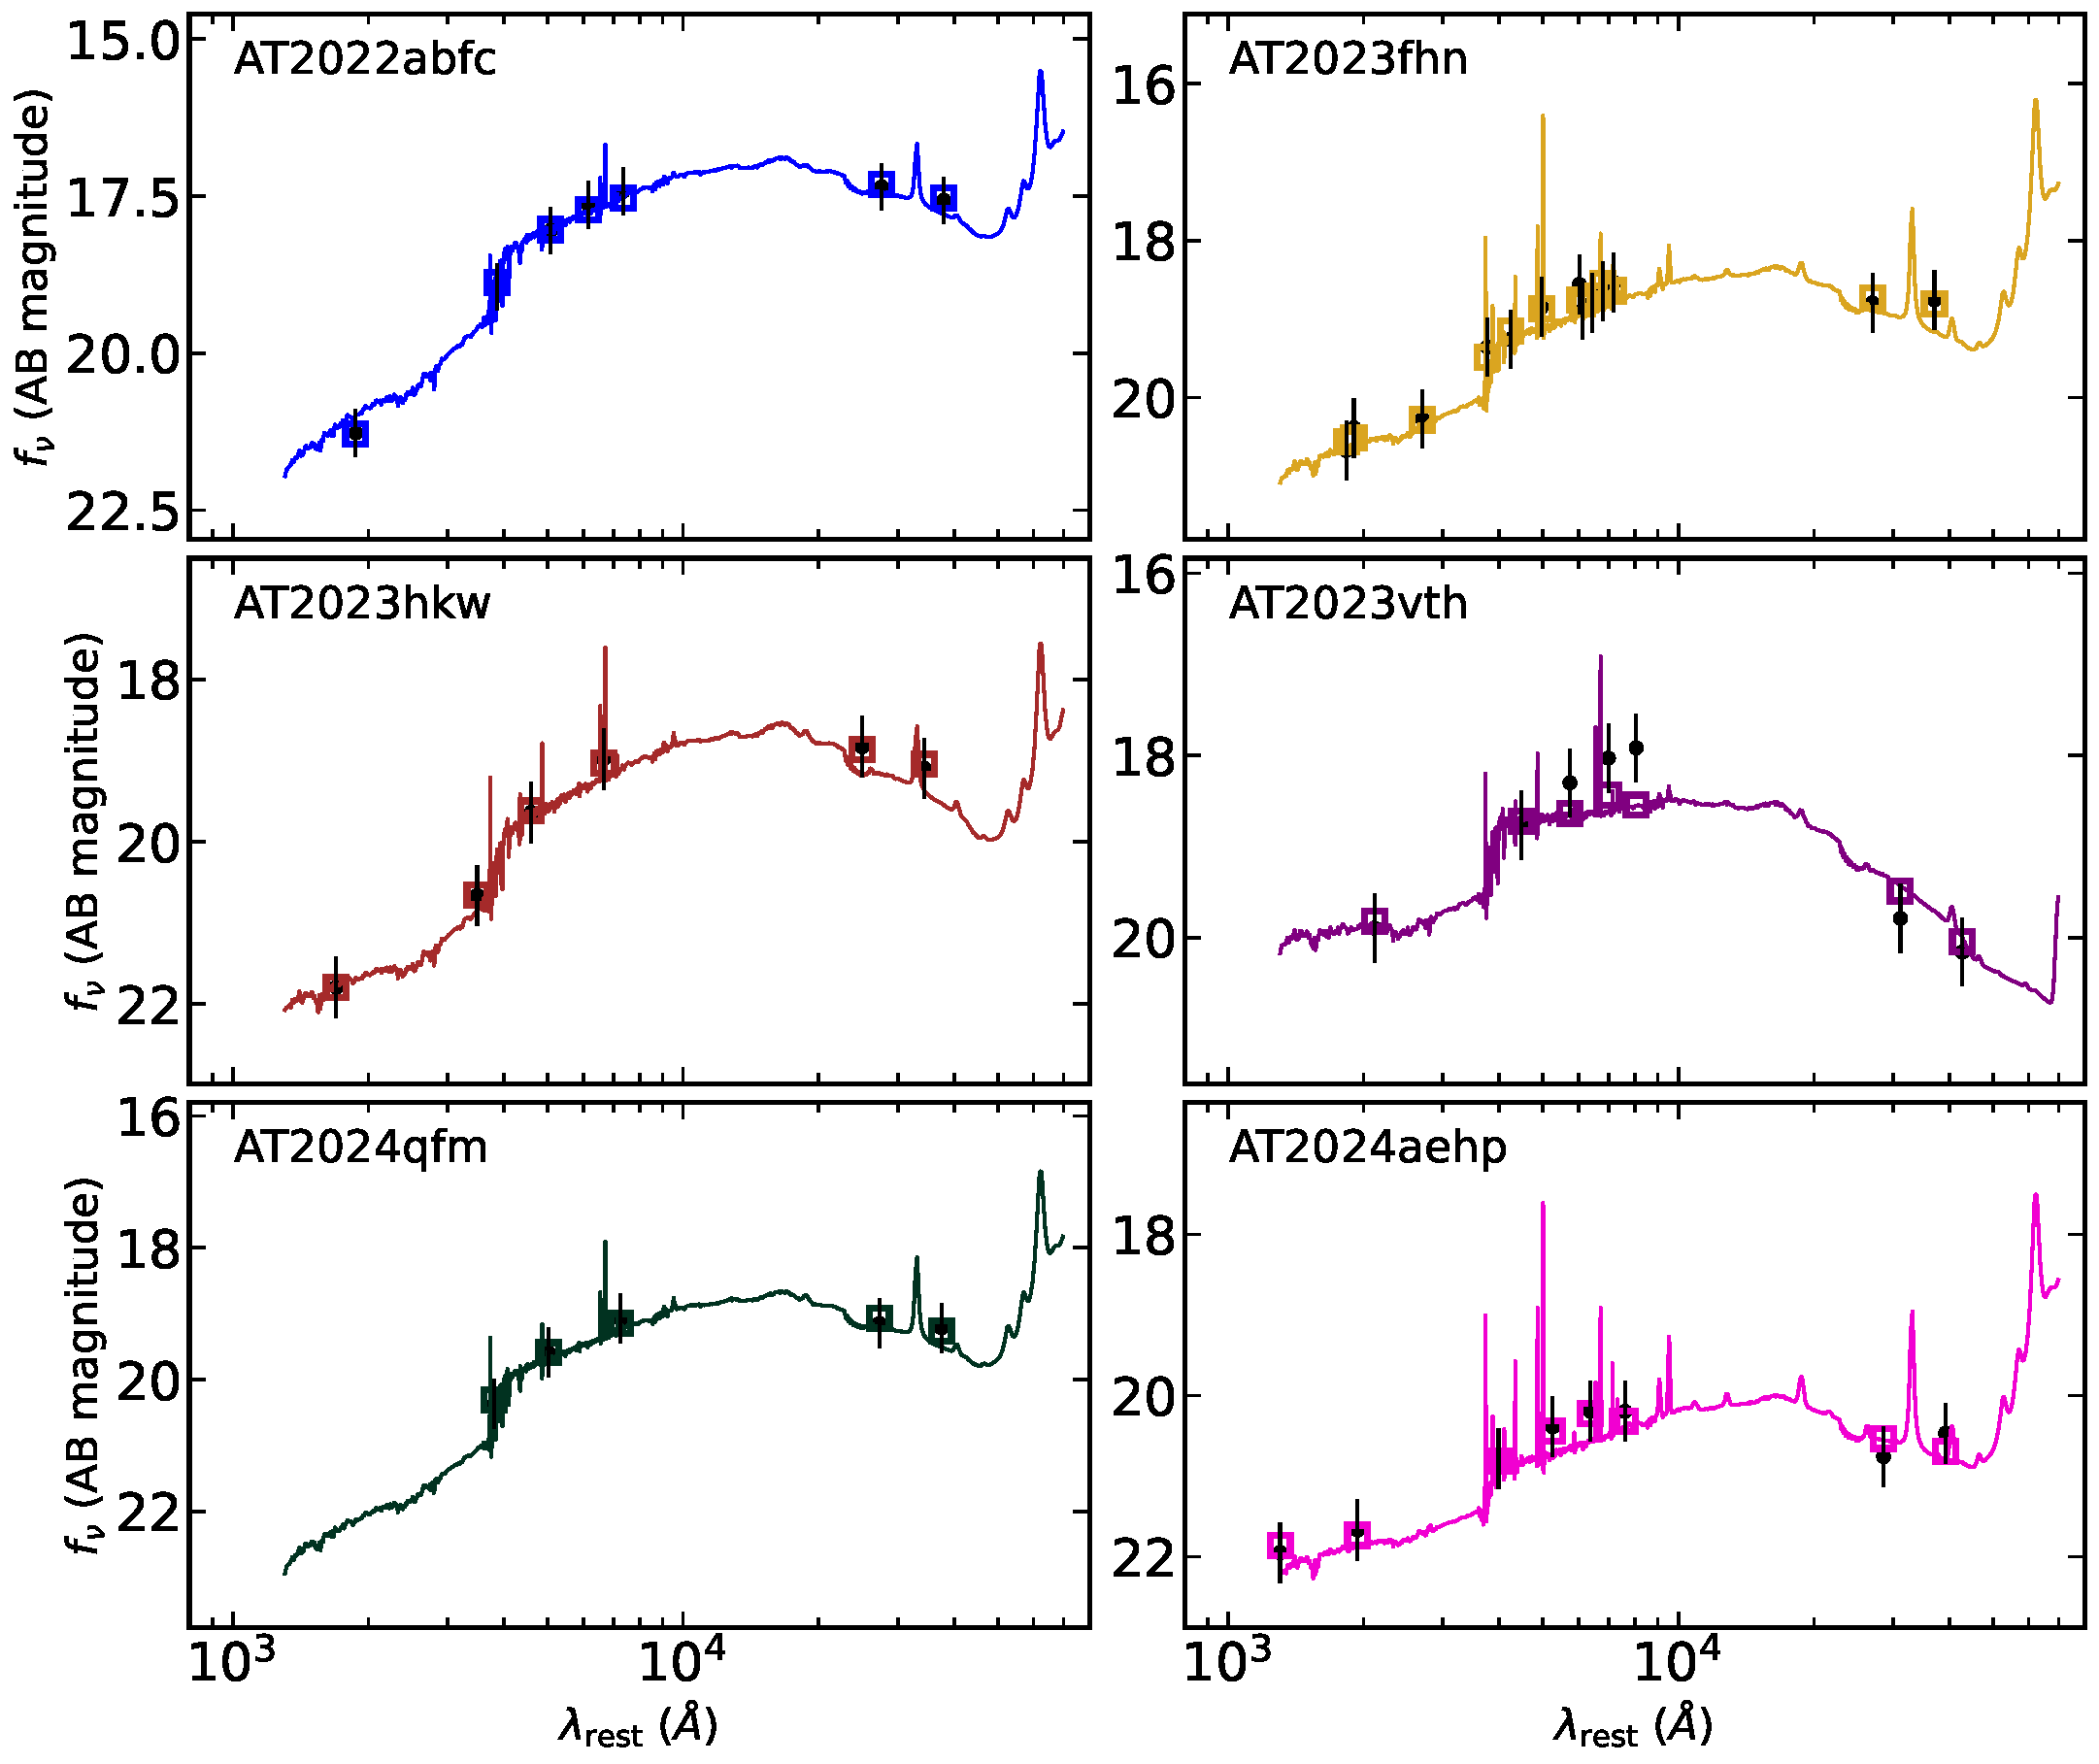
\includegraphics[width=\linewidth]{fig10_specfit.pdf}
\caption{Best-fit host-galaxy spectra and photometry from \texttt{prospector} (color) as well as the input photometry (black circles with error bars).  Note that the parameters reported in Table~\ref{tab:galaxy_prop} are the median, 16th percentile, and 84th percentile.  The best-fit host galaxy spectra displayed here corresponds to the maximum {\bf a posteriori model}, which {\bf may not necessarily have} the median parameters.  The abscissa 
%$x$-axis 
displays rest-frame wavelength.}
\label{fig:spec_fit}
\end{figure*}

\begin{figure}[!h]
 \centering
  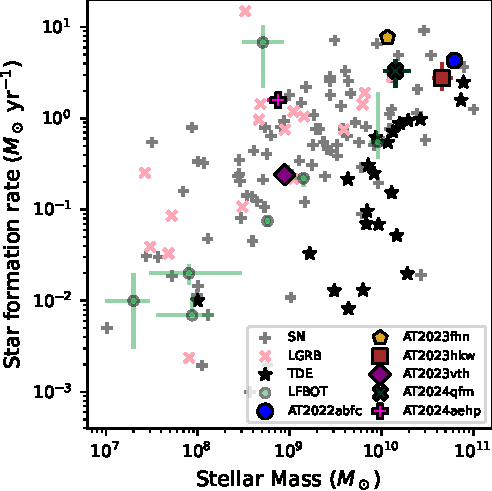
\includegraphics[width=\linewidth]{fig11_host_galaxy.pdf}
\caption{Median mass and 
%star formation rate 
SFR for each LFBOT's host galaxy in comparison to the host galaxies of other energetic transients.  Colored lines show error bars, though they may be smaller than the marker for some points.  \added{Data for the other transients from \citep{lawsmith2017, french2020, taggart2021, Somalwar2025}.}}
\label{fig:host_galaxy}
\end{figure}


\subsection{Host-Galaxy Properties}\label{sec:host}

We used the Python package \texttt{prospector} \citep{prospector1, prospector2}\footnote{\url{https://github.com/bd-j/prospector}} to derive properties such as stellar mass and star-formation rate (SFR) from the host-galaxy photometry.  The \texttt{prospector} package utilizes the Flexible Stellar Population Synthesis\footnote{\href{https://dfm.io/python-fsps/current/}{https://dfm.io/python-fsps/current/}} (FSPS) package to model the emission from each galaxy given a set of parameters for the galaxy's composition and stellar population. \added{It also utilizes dynamic nested sampling through the package \texttt{dynesty}\footnote{\href{https://github.com/joshspeagle/dynesty}{https://github.com/joshspeagle/dynesty}} to fit galaxy parameters to the observed galaxy photometry under Bayesian inference.}  The basic parametric star-formation history template is adopted along with the parameters for nebular emission.  We chose the Chabrier initial mass function \citep{chabrier2003}, the Calzetti dust attenuation model \citep{calzetti2000}, and a star-formation history of the form $t e^{-t/\tau}$.  \added{These procedures were chosen to match LFBOT host galaxy analysis in previous papers as closely as possible \citep{yao2022, ho2023tsd, chrimes2024}.} A model was first run with a fixed metallicity of $\log (Z/Z_{\odot})=-0.2$.  Then, we used the median mass and the mass-metallicity relation of \citet{gallazzi2005} to fix the metallicity to a more accurate value, and ran a final model.
The fitted parameters are listed in Table~\ref{tab:galaxy}, the best-fit photometry and spectroscopy are displayed in Figure~\ref{fig:spec_fit}, and the fitted host-galaxy properties are listed in Table~\ref{tab:galaxy_prop}.  We show the median host-galaxy masses and SFRs in Figure~\ref{fig:host_galaxy}.  Our host-galaxy properties derived for the host of AT2023fhn agree with \citet{chrimes2024} to within 1-$\sigma$ for \added{the} host-galaxy mass and 2-$\sigma$ for \added{the} SFR. 

The host galaxies of our LFBOTs are all star-forming galaxies. Whereas several previous events were in low-mass dwarf galaxies \citep{ho2020koala, coppejans2020,chrimesfhn,margutti}, the host galaxies of four of our new LFBOTs have higher masses ($10^{10}$--$10^{11}\,M_{\odot}$, Figure~\ref{fig:host_galaxy}). However, our selection criteria for identifying LFBOT candidates do require there to be a visible host galaxy (to avoid contamination by dwarf novae), so a bias to higher mass galaxies \added{(and therefore higher star-formation rate)} is to be expected. 

To compare the \emph{intrinsic} distribution of host-galaxy mass to that of CCSNe, we used the untargeted sample of 150 CCSN host galaxies from \citet{taggart2021} as representative of the true CCSN host galaxy population.  \added{We prioritized having an unbiased sample over a large comparison sample, as our uncertainties are limited by our small LFBOT sample.}  For each of the thirteen LFBOT host galaxies, we calculate the minimum absolute magnitude for it to have been detected by the Legacy Survey at that redshift, which corresponds to the apparent magnitude cutoff of $\mathrm{m}_r\leq23$.  Then, for each CCSN host galaxy, we apply a weight equal to the proportion of the thirteen cutoffs that the CCSN host galaxy would pass. We do not account for any systematic differences in host galaxy properties between those at redshift $z\approx 0.01$ as in the Taggart sample, and those at $z\approx 0.1$--0.2 as with most of the LFBOTs.  We plot the Gaussian kernel density estimation (KDE) for the weighted distribution of CCSN host-galaxy masses Figure~\ref{fig:host_galaxy_sim} as a dotted red line.  The Gaussian KDE for the LFBOT host-galaxy masses is shown in black. We repeated the exercise for SLSNe, which are known to have a preference for lower galaxy masses than regular CCSNe \citep{taggart2021}.

%For each ``trial,'' we randomly selected 13 galaxies out of the 150 and placed them at the redshifts of the 13 LFBOTs in Table~\ref{tab:summary}. We required that each CCSN host galaxy be luminous enough to be detected at that redshift by the Legacy Survey ($\mathrm{m}_r\leq23$; \citealt{legacy}). If the galaxy was not sufficiently luminous, we removed it and drew a new random galaxy. We repeated this process 1000 times to create a large number of $N=13$ CCSN host-galaxy sub-samples. We plot the Gaussian kernel density estimation (KDE) for the distribution of host-galaxy masses for each of these subsamples in Figure~\ref{fig:host_galaxy_sim} as gray lines.  These would be the distributions of host-galaxy masses we would expect for the observed LFBOTs {\em if} the LFBOT host galaxies are identical to CCSN host galaxies, accounting for the selection effects from requiring a visible host galaxy for our LFBOT candidates.  The red lines show the 25th, 50th, and 75th percentiles of these Gaussian KDEs.  The Gaussian KDE for the actual LFBOT host-galaxy masses is shown in black. We repeated the exercise for SLSNe, which are known to have a preference for lower galaxy masses than regular CCSNe \citep{taggart2021}. 

 %We do note that the median redshift of the galaxies in the \citet{taggart2021} sample is $z\approx 0.01$, which is less than the $z\approx 0.1$--0.2 redshifts of most of the LFBOTs.  We make no correction to account for possible differences between galaxies at different redshifts.

%We also account for our bias requiring a detected galaxy for an LFBOT classification.  This is done by creating a large number of random subsamples of the CCSN hosts that each contain thirteen host galaxies.  Each galaxy in the subsample is matched to an LFBOT and its redshift.  

\begin{figure*}[!htb]
 \centering
  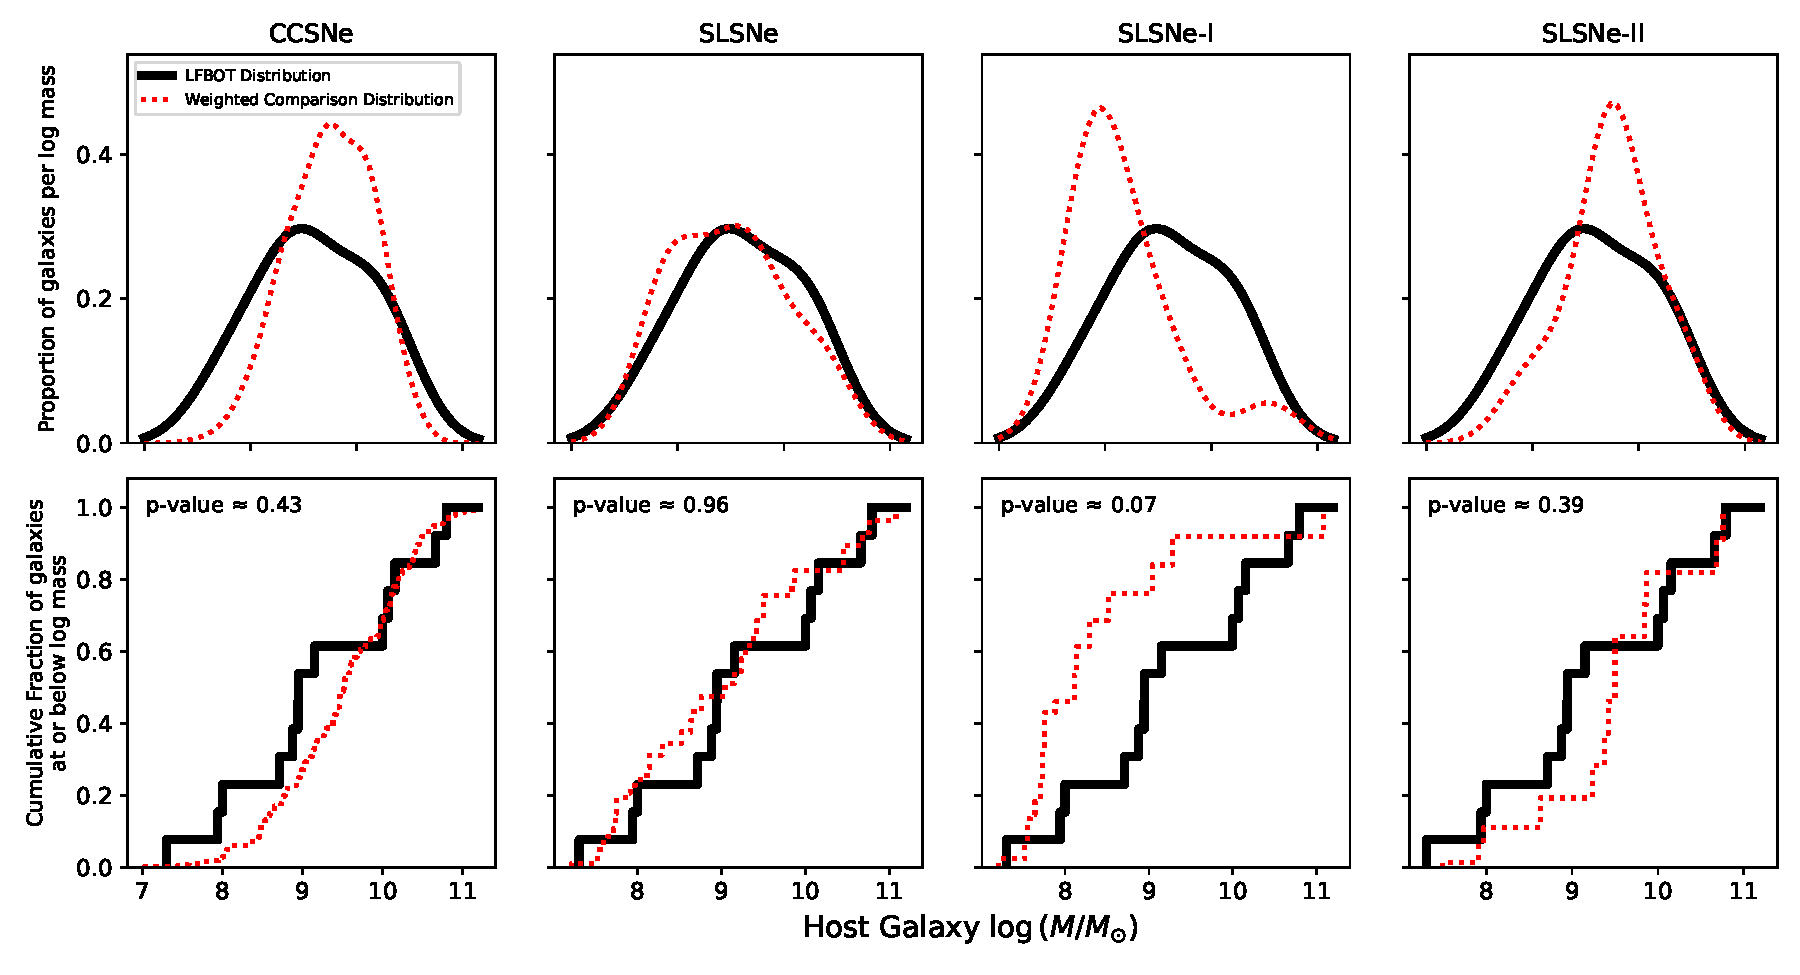
\includegraphics[width=1.0\linewidth]{fig12_host_galaxy_sim_all.pdf}
\caption{Gaussian KDEs for the LFBOT host-galaxy masses (black) in comparison to the Gaussian KDEs for each of the weighted mass distributions from the \citet{taggart2021} CCSN/SLSN host-galaxy population (dashed red).  \bf{We also list the p-values from our Kolgomorov-Smirnov test.}}
\label{fig:host_galaxy_sim}
\end{figure*}

%While this paper also included a sample of LGRB host galaxies, it is too small for a reliable analysis.

We use the \texttt{Ecume} package \citep{ecume} in the programming language \texttt{R} \citep{r} to perform a Kolmogorov-Smirnov (KS) test comparing the distribution of LFBOT host-galaxy masses with the weighted CCSN and SLSN populations.  These simulations imply that the LFBOT host-galaxy population is consistent with both the populations of CCSN and SLSN host galaxies at a significance of $\alpha=0.05$ (\added{which means that the p-value must be less than $0.05$ for us to conclude that the underlying distributions are different with 95\% confidence}).  \added{We also display the results of the KS test in Figure~\ref{fig:host_galaxy_sim}}. The SLSN host-galaxy distributions appears especially similar to that of LFBOTs. However, the SLSNe are subdivided into SLSNe-I and SLSNe-II.  These two classes are markedly different, and this is reflected in their host-galaxy masses---SLSN-I host galaxies are clustered around $\log \,(\mathrm{M}/\mathrm{M}_{\odot})\approx 8$ while SLSN-II hosts are $\log \,(\mathrm{M}/\mathrm{M}_{\odot})\approx 9$--10.  Despite the visible differences, the sample sizes of SLSN-I and SLSN-II hosts are too small to find a statistically significant difference at $\alpha=0.05$.  %The KS test finds that the LFBOT host-galaxy mass distribution is inconsistent with that of SLSN-I and SLSN-II host galaxies.   %We must also caution that there are only 37 SLSN hosts in the \citet{taggart2021} sample. 

%\begin{deluxetable}{cc}%[!h]\label{tab:kstest}
%\setlength{\tabcolsep}{3.6em}
%\tablewidth{\textwidth}
%\tabletypesize{\footnotesize}
%\tablecaption{Kolmogorov-Smirnov Test for %Host-Galaxy Masses}
%\tablecolumns{2}
%\tablehead{
%\colhead{Comparison %Population}&\colhead{$p$-value}}
%\startdata
%CCSN &  0.43\\
%SLSN &0.96\\
%SLSN-I & 0.07\\
%SLSN-II & 0.39\\
%\enddata
%\vspace{-0.1mm}   
%\tablecomments{Results of a two-tailed %Kolmogorov-Smirnov test between the LFBOT %host-galaxy mass distribution, and the host-%galaxy mass distributions of four %populations (CCSN, SLSN, SLSN-I, SLSN-II).}
%\end{deluxetable}

%There are important caveats to our statistical analysis above.  Firstly,  Secondly, we note that \citet{taggart2021} only examine 37 SLSN host galaxies.  As we are drawing thirteen galaxies for each subsample, our results largely reflect the properties of the 37 galaxy sample, which is susceptible to small sample-size effects.  

%Combined with the analysis of host galaxy offsets in Section~\ref{sec:offset}, this suggests that out of the common classes of explosive transients, super-luminous supernovae could be the closest analogues to LFBOTs.

 %If LFBOTs are of the same character as SLSNe, LFBOTs could also be split into analogous subgroups.  However, the remarkable consistency of some LFBOT characteristics, particularly the radio and millimeter emission, makes this unlikely.

\section{Discussion}
\label{sec:discussion}

\subsection{Observational Comparison}
\label{sec:comparison}

The objects presented in Section~\ref{sec:methods} show relative homogeneity in the optical (Figure~\ref{fig:optical}) and radio (Figure~\ref{fig:radio-lc}) light curves. To some extent the similarity of the optical light curves to those of AT2018cow is by selection, as these objects were identified on the basis of a rapid rise and decay \added{within the 2--3 days of the optical peak,} along with high luminosities. %However, for selection the optical light curve only needed to decline to half-maximum light within a short period of time. 
The rapid decline of 3--4 mag over $t_\mathrm{rest}\approx10\bf{-15}$\,d observed in AT2023fhn, AT2023vth, AT2023hkw, and AT2024qfm --- very similar to AT2018cow --- was not selected for.  
\added{We note that AT2024aehp differs in many of these properties.  This section will focus on the other LFBOTs in our sample; AT2024aehp will be discussed in more detail in Section~\ref{sec:24aehp}.}

\added{While the other optical light curves could appear similar due to selection effects, selection effects do not account for the similarity between the LFBOT radio light curves as we only require one detection for classification.} Figure~\ref{fig:radio-lc} shows that the peak $\nu L_{\nu}$ values mostly lie within the range of $10^{39}$--$10^{40}$\,erg\,s$^{-1}$. The time evolution for the radio emission is also similar across the sample.  The 10\,GHz luminosity gradually rises, plateaus between $t_{\mathrm{rest}}\sim50$--100\,d after the initial discovery, and then begins to fade. During the rise, the radio emission is typically optically thick (has a positive spectral index; Figure~\ref{fig:radio-sed}). The \added{decay} rates of the radio emission vary, and in some cases are poorly constrained (e.g., for AT2022abfc). The fast fade of AT2023vth is similar to that of CSS161010 \citep{coppejans2020}. \added{Meanwhile}, the mm-wave light curves appear to peak close \added{at times close} to $t_{\text{rest}}=20-30\,$d (Figure~\ref{fig:mm}).  \added{All SEDs either have or are consistent with a broken-power law shape.  The frequency is near 50\,GHz during the first detections at $t_{\mathrm{rest}}\sim30$\,d, then gradually shift to lower frequencies, passing 10\, GHz at roughly $t_{\mathrm{rest}}\sim100$\,d.}

The uniformity of the radio luminosity and evolution of all AT2018cow-like FBOTs is striking. Of course, the radio emission had to be sufficiently luminous to be detected in the first place, but we did not require the radio luminosity to brighten over time, nor was there a requirement about the timing of the peak. The radio behavior is in sharp contrast to CCSN 
%core-collapse supernova 
radio light curves, which span over four orders of magnitude in luminosity, with peak times ranging from a few days to thousands of days \citep{Bietenholz2021}.  \added{This diversity suggests that core collapse supernovae occur with a wide range of CSM densities and spatial distributions.  As this is not the case for LFBOTs, we conclude that the CSM properties must be tied to the LFBOT progenitor channel.  We discuss the implications of this further in Section~\ref{sec:discussion-progenitors}.}

We have fewer constraints on the X-ray behavior, as several of the objects only have upper limits on their luminosity (the calculated X-ray luminosity upper limits are driven mostly by their redshift, as \swift\ determined similar photon count upper limits for each non-detection).  \added{But as seen in Figure~\ref{fig:xray},} these upper limits appear to rule out X-ray emission similar to those of jetted TDEs or classical LGRBs while allowing for the possibility of X-ray emission similar to that of AT2018cow.  \added{In addition}, the order-of-magnitude jump in X-ray luminosity seen in AT2024qfm over just two days is much more pronounced than the X-ray variability observed in past LFBOTs. 

\subsection{Implications for Progenitors}\label{sec:discussion-progenitors}

%\subsection{X-ray}
%A consistent feature through all AT2018cow-like FBOTs with conclusive X-ray detections is the incompatibility between the X-ray spectrum and the synchrotron spectrum derived by radio observations \citep{margutti,coppejans2020,yao2022}.  There has always been an observed X-ray excess over an extension of the radio spectrum.  X-ray radiation is also found to be inconsistent with Inverse Compton scattering of the optical radiation \citep{margutti,yao2022}.    For the LFBOTs in this paper without previous X-ray observations, we can check if the \swift\ upper limits are consistent rule out this excess.  This is predicated on a thorough fit of the radio data to a synchrotron spectrum.

%\subsection{Summary}

%With the exception of AT2024aehp, these LFBOTs have similar radio and optical light curves.  The radio observations in particular are very similar across this sample, with similar luminosities and timescales at 10\,GHz and 100\,GHz. The similarity in optical emission can be explained to some extent by the fact that we require certain characteristics in the optical light curve to classify a transient as an LFBOT --- however, we do not require continued fast fading as seen in several events (and not seen in AT2024aehp). 

%There is even less of a selection bias for the radio emission, as we only require a single radio detection for classification.  There is no reason to be biased toward transients with the pattern of radio emission displayed in Figures \ref{fig:radio-lc} and \ref{fig:radio-sed}: a broken power-law SED continuously shifting to lower frequencies, reaching maximum intensity at $t_{\text{rest}} \approx 50$--100\,d days when the peak frequency is near 10 GHz, then fading.  %The shape of the radio SED implies that it is synchrotron radiation produced by a shock interacting with a dense medium.  
 %, which can be seen in Figure~\ref{fig:synchrotron} and Table \ref{tab:synchro}.  %The derived circumstellar medium density is consistent with a stellar wind with a mass loss rate on the order of $10^{-4}\,M_{\odot}\,\mathrm{yr}^{-1}$ assuming a wind velocity of $1000\,\text{km}/\text{s}$.

%\begin{figure}[!htb]
% \centering
%  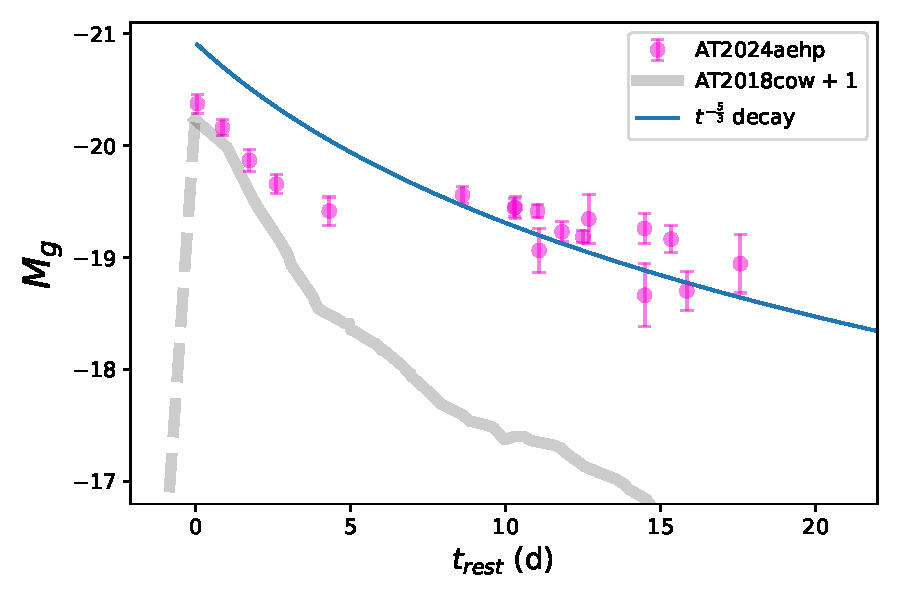
\includegraphics[width=0.9\linewidth]{fig13_aehp_lc.pdf}
%\caption{Optical $g$-band light curves for AT2024aehp (pink points) and AT2018cow (gray line).  AT2018cow represents a typical LFBOT light curve.  We also show a best fit of a $t^{-5/3}$ decay to the AT2024aehp light curve\added{, as that is the canonical optical decay timescale for a TDE \citep{evans1989}}.  The time axis is measured in the rest frame \ of each transient, where $t_{\text{rest}} = 0$ refers to the peak of the optical light curve.}
%\label{fig:aehp_lc}
%\end{figure}

The consistent radio light curves imply consistent properties of the surrounding medium on scales of $\sim 10^{16}$--$10^{17}\,$cm. \added{Assuming this medium was produced by material ejected from the progenitor at 1000\,km\,s$^{-1}$, it probes timescales of a few to tens of years prior to the transient's explosion. Therefore, the radio behavior favors progenitor theories that can explain the presence of a dense ambient medium that is fairly similar from event to event and is produced well in advance of the explosion. This is hard to reconcile with a TDE scenario.  \citet{margutti} finds that the IMBH invoked to explain LFBOTs are unable to sustain outflows sufficient to produce this medium.}  %A TDE must either produce a medium of the required density, which is difficult \citep{margutti}, or always occur in an existing dense medium, which is hard to justify.  %Additionally, TDEs are rarely off-nuclear, unlike LFBOTs.
Difficulties also arise in the massive-star core-collapse model: the stars that we usually suspect to be the progenitors of luminous explosions and energetic SNe are not expected to undergo significant mass loss in such a consistent way just prior to the explosion (indeed, SN radio light curves are highly diverse).  %Models of LFBOT host galaxy properties also indicate a discrepancy between the LFBOT and CCSNe host galaxy populations.  
On the other hand, progenitor models involving mergers \citep[e.g.,][]{metzger2022,Tsuna2025,Klencki2025} naturally explain the dense medium as material ejected from the merger.   \added{Each proposed merger scenario involves mass transfer from a massive donor star to a compact object.  These papers estimate the circumburst medium density from calculations of the stellar wind from the donor star and mass-loss during the merger, and have found them to be consistent with density estimates from past LFBOT papers.  These estimates are also expected to hold for each instance of such a merger, explaining the consistency across the LFBOT sample.}  %, along with the locations in star-forming galaxies.

\subsection{AT2024aehp}\label{sec:24aehp}
AT2024aehp has several characteristics that distinguish it from the other LFBOTs in this paper. Its optical light curve exhibited a plateau \added{at $M=-19$\,mag from 5--50\,d, behavior we can rule out in AT2023vth and AT2024qfm but not in AT2022abfc, AT2023fhn, and AT2023hkw. AT2024aehp is also an outlier in terms of radio evolution. As shown in Figure~\ref{fig:radio-lc} and Figure~\ref{fig:radio-sed}, AT2024aehp dramatically brightens in radio luminosity at a later time than the other transients we have discussed, by over an order of magnitude in all frequencies between the $t_{\mathrm{rest}}\sim70\,$d and $t_{\mathrm{rest}}\sim120\,$d epochs. In contrast, the radio emission of other LFBOTs has already peaked by $t_{\mathrm{rest}}\sim120\,$d and begun to shift to lower frequencies.}  \added{AT2024aehp is also one of only two LFBOTs to have a localization that is consistent with it being a nuclear transient (the other being CSS161010)}. 

\added{The properties of AT2024aehp} are reminiscent of TDEs. 
\added{Most observed TDEs occur in the nucleus as they involve the galaxy's central supermassive black hole \citep{gezari2021}},  exhibit late-time radio brightening \citep{horesh2021, cendes2024}, and have a slower optical light-curve decay following $t^{-5/3}$ \citep{evans1989}.  While known TDEs have optical rises lasting weeks \citep{blagorodnova2017}, a TDE from an intermediate-mass black hole could have a much shorter rise \citep{kuin2019,perley2019,Gutierrez2024}.
Indeed, the transient AT2024puz---which produced luminous optical/UV evolving on a $\approx20\,$d timescale as well as luminous ($10^{44}\,$erg\,s$^{-1}$) X-ray emission---was posited to be an object intermediate between LFBOTs and TDEs \citep{Somalwar2025}. Observations of AT2024aehp are ongoing, and a detailed analysis of this transient will be presented in future work.   

%Still, there are some discrepancies.  AT2024aehp's optical plateau does not fit the  $t^{-5/3}$ power law (Figure~\ref{fig:aehp_lc}).  Furthermore, TDEs showing late radio brightening have SEDs with a peak frequency lower than 10 GHz about 100 days after peak light \citep{horesh2021, stein2021}.  
%While AT2024aehp may be a TDE, these differences warrant a further investigation into this transient.  

\subsection{Considerations for Future Work}\label{discussion-improvements}


From our work discovering and performing multiwavelength observations of LFBOTs, we have identified areas to improve on for future analysis, summarized below. %These can be broadly divided into three categories: performing follow-up observations, modeling, and sampling transient populations.

{\em Observations} -- %Although it is too early to tell if AT2024aehp's characteristics will be replicated in other LFBOTs, it is important to ensure we would be able to detect them if they occur.  
\added{It is unclear how prevalent optical plateaus and late-time radio rebrightenings (as was seen in AT2024aehp) are in LFBOTs.} The optical light curve plateau of AT2024aehp motivates long-term ($>10\,$d) optical monitoring of LFBOTs. As shown in Figure~\ref{fig:optical}, this extended follow-up was not present in our sample's early LFBOTs \added{AT2022abfc, AT2023fhn, and AT2023hkw}, which limits our ability to constrain the presence of a similar plateau.  \added{In addition, late-time radio follow-up observations should be obtained to search for  rebrightenings on timescales of hundreds of days.}

Another gap in our follow-up observations is the lack of X-ray detections for most of these LFBOTs. \swift\ observations were not sensitive enough to rule out levels of X-ray emission that have already been detected in previous LFBOTs such as CSS161010 \citep{coppejans2020} and AT2018cow \citep{perley2019}.  Going forward, deeper {\em Chandra} observations should be obtained for each object, as was done in, e.g., AT2023fhn \citep{chrimes2024}.  \added{X-ray detections will let us verify that the X-ray emission is in excess of the extrapolated synchtrotron SED, confirming that it originates from a different source, like in previous LFBOTs \citep[e.g.][]{margutti, bright2022}.  This also allows us to track the ratio of X-ray to UV/optical flux over time.  Under the proposed scenario that the UV/optical flux is reprocessed high-energy radiation \citep{margutti, lebaron2025}, this would enable us to track the optical depth of the ejecta's reprocessing layer.  Finally, as the X-ray flux is thought to originate from a central object \citep{ho2019, metzger2022, nayana2025}, it is one of the few probes of the regions closest to the transient's center.}

{\em Modeling} -- The models we use in this paper's analysis could be improved upon or have assumptions that could be relaxed to explore a wider range of parameter space.  

We use the model of \citet{chevalier} to derive properties of the shock and ambient medium from our radio and millimeter observations.  This formulation requires assuming that certain conditions hold, such as the equipartition of energy, a non-thermal electron energy distribution, and that the shock is spherical and nonrelativistic.  The nonrelativistic assumption will introduce some inaccuracies, as we calculate some values of $\Gamma \beta$ that are greater than 0.5.  We also assume values for the filling factor $f$, $\epsilon_e$, $\epsilon_B$, and the electron power-law index, and our results do depend on these parameters. % The equations in \citet{chevalier} show that our results do depend sensitively on these parameters.  
A future analysis could relax some of these assumptions or fit for parameters that we set to be fixed.  Some of these flaws can be inferred from our fitting results.  According to \citet{chevalier}, the broken power-law fit should have a $\nu^{5/2}$ dependence in the optically thick regime and a $\nu^{-(p-1)/2}$ dependence in the optically thin regime, where $p$ is the electron power-law index.  We assume $p=3$, so the optically thin dependence should be as $\nu^{-1}$.  However, for most epochs we do not have enough detections to confirm a $\nu^{5/2}$ dependence in the optically thick regime (Figure~\ref{fig:radio-sed}).  In addition, from the results shown in Table~\ref{tab:synchro_fit}, the observed slopes in the optically thin regime are not all consistent with $\nu^{-1}$.  Work has already been done to extend this model to account for thermal electrons \citep{margalit2021} and relativistic effects \citep{margalit2024, ferguson2025}.  Generalizing and refining the synchrotron model would help obtain more rigorous estimates of shock and ambient medium parameters.  \added{For example, relativistic effects become significant at $\Gamma \beta \gtrsim1$---which some of our LFBOTs approach---where results can differ by an order of magnitude \citep{ferguson2025}.  Our conclusions would still be applicable as they rely on the similarity of the radio emission between LFBOTs, but our numerical results can be significantly affected.  As our paper's scope is to present new observational data for six LFBOTs and use techniques analogous to those in previous LFBOTs papers to compare properties across this sample, we defer the application of improved synchrotron radiation models to future work.} %, and would also be relevant for studies on radio emission from other transients such as SNe or GRBs.

In our \texttt{prospector} fits for the LFBOT host-galaxy properties, we used a single prescription for the SFH, dust model, and initial mass function, but a future analysis should ensure that results are robust to different choices for these parameters.  In particular, we use a parametric SFH to \added{match the work of previous LFBOT papers, but internal testing with a non-parametric SFH produced results that differ by about 1-$\sigma$}.  We also omit the spectra when performing our fits, as it is difficult to standardize spectra from different observing conditions, processed through different software, and possessing different levels of contamination from the transient itself.  This required us to use the mass-metallicity relation in \citet{gallazzi2005} to fix a metallicity in our models.  \added{As the mass is largely set by the galaxy's overall luminosity, we expect that this would lead to little change in our mass estimates, but will bias our metallicity estimates to more moderate values.  We have also observed that the star-formation rate estimate is insensitive to changes in metallicity.  So, our method does introduce a caveat to our metallicity estimates, but we still have confidence in our host-galaxy analysis as it relies on the mass and star-formation rate.  Still, }incorporating a host-galaxy spectrum obtained after the transient faded would produce a more accurate result.  \added{After the submission of this paper, \citet{Nugent2026} performed a \texttt{prospector} LFBOT host-galaxy analysis with a non-parametric star-formation history and utilized host-galaxy spectrscopy when available.  They find similar results for the hosts of AT2023fhn and AT2024qfm, but have larger host-galaxy masses by a factor of a few for AT2023hkw and AT2023vth.}


{\em Selection Bias} -- \added{
%We make no claims that our LFBOT sample is complete or unbiased.  
Our requirements for LFBOT classification introduce biases that are difficult to account for.}  For example, the requirement of a visible host galaxy biases our sample towards more luminous hosts.  %While our analysis in Section~\ref{sec:host} demonstrates some techniques we can use with a larger sample size, a proper statistical analysis and comparisons of transient populations require us to fully account for biases in the construction of our LFBOT sample.} We must also do the same for \added{samples of other transient classes that we use as a comparison}.  Ensuring that a sample is representative is especially difficult for rarer classes of transients.
While we did account for some bias in our LFBOT sample in our study on host-galaxy masses, we \added{caution that we }did not perform any such correction for our analysis of host-galaxy offsets. %\added{, so our results should be taken with a grain of salt}.  
\added{Another source of bias is our requirement of an X-ray and radio detection.  While this would exclude LFBOTs that are X-ray and radio faint, our procedure's success rate of detecting X-rays or radio emission from promising LFBOT candidates implies that the loss is not significant.  Finally, all of these LFBOTs were selected on the basis of their optical light curves.  As we discussed in Section \ref{sec:comparison}, this would bias our LFBOTs to have similar optical light curve properties, such as their absolute luminosities and rise/\added{decay} rates.  This could lead us to miss any diversity in LFBOT optical characteristics (e.g., \citealt{Somalwar2025}).}  %We also do not account for any redshift evolution in galaxy properties, which we expect to occur even at $z<1$ \citep{lilly1996}.  
%Representative samples of a variety of transient classes in larger numbers and a broader span of redshifts will be necessary to rigorously perform this type of analysis.

\emph{Future Surveys} -- The development of the Vera C. Rubin Observatory \citep{lsst} and its deep, wide-field optical imaging survey is expected to increase the transient discovery rate by orders of magnitude. This would cause the number of known LFBOTs to increase significantly, paving the way for more robust analysis. The results presented in this paper inform how to best handle each new LFBOT discovery and serve as a blueprint for statistical analysis of an expanded LFBOT sample. 

Rubin data, along with the advent of high-cadence wide-field UV surveys such as the Ultraviolet Transient Astronomy Satellite (ULTRASAT; \citealt{Shvartzvald2024}) and the Ultraviolet Explorer (UVEX; \citealt{Kulkarni2021}), will enable LFBOTs to be identified and followed up much earlier in their evolution.  \added{Rubin's sensitivity can allow for detections before the optical peak, allowing us to identify rapid rising light curves within a couple of days.  Photometric classifiers can potentially screen out LFBOT false positives, mitigating the dependence on the presence of a host galaxy for classification.    Meanwhile, ULTRASAT's rapid cadence (5 minutes) means that an LFBOT's fast brightening can be identified in a matter of hours.   Faster discoveries enable earlier radio observations at $t_\mathrm{obs}\leq5$ days, probing smaller shock radii and more recent mass-loss history.  %An LFBOT's rising UV light curve would be an entirely new facet of the transient; none of the LFBOTs in Table~\ref{tab:summary} have had such observations.  
Early UV observations, in conjunction with NIR observations, can show evidence of a dust echo, providing an independent measure of the surrounding CSM \citep{metzger2023}.  The UV can also provide better estimates of the early photospheric radius and effective temperatures, as fits to only optical detections can be uncertain \citep{Pursiainen2025}.  Additionally, time-domain surveys outside the optical band can provide a new avenue to find LFBOTs.  %Any such method would not be susceptible to the past selection bias for a specific kind of optical light curve.  
These surveys may show that LFBOTs are part of a more diverse sample that we have only begun to study.  In all, the ability to detect and study LFBOTs over a broader suite of observatories and surveys can remedy some of the challenges of our current studies.}  

%LFBOTs discovered by Rubin and other upcoming time-domain surveys could unravel the true nature of this class of transients.

\section{Summary}

We presented multiwavelength data---including optical photometry, optical spectroscopy, \emph{Swift} X-ray observations, and VLA/NOEMA/uGMRT radio observations---of six LFBOTs (AT2022abfc, AT2023fhn, AT2023hkw, AT2023vth, AT2024qfm, and AT2024aehp) at redshifts spanning $z=0.0747$--0.339. We identified all of these objects on the basis of fast light-curve evolution in ZTF survey data, and confirmed their similarity to the prototype AT2018cow via radio detections. Five of the six LFBOTs (all except AT2023fhn) are presented here for the first time. Our work increases the known number of LFBOTs by 50\%. 

The optical light curves of four \added{of these} events fade by 3--4\,mag over $t_\mathrm{rest}\approx10\,$d, similarly to AT2018cow. A fifth event, \added{AT2022abfc, did not have deep photmetric follow-up to confirm fading over this timescale, but had a similar decay rate over the first five days.  The last,} AT2024aehp, exhibited a plateau at $M\approx-19\,$mag over tens of days, after an initial fast decline. The optical spectra do not show any clear features from the transients themselves, including a spectrum of AT2024aehp during its plateau phase. 

The X-ray luminosity of AT2024qfm is among the highest of all LFBOTs to date, at $10^{44}\,$erg\,s$^{-1}$ at $t_\mathrm{rest}\approx1\,$week. The X-rays also appeared to show a brightening by an order of magnitude over just a few days. \emph{Swift} X-ray observations of the other objects resulted in non-detections that were not deep enough to rule out emission identical to AT2018cow itself. AT2023fhn was detected by Chandra at similar levels to AT2018cow \citep{chrimesfhn,nayana2025}. 

The 10\,GHz radio light curves peak at $t_\mathrm{rest}\approx50$--100\,d, with peak luminosities primarily in the range of $10^{39}$--$10^{40}$\,erg\,s$^{-1}$. During the rise, the emission appears to be self-absorbed, confirmed by multi-band VLA observations, as well as by NOEMA 100\,GHz detections for AT2024qfm and AT2023vth. We measured basic shock parameters using a simple equipartition analysis, and found---as for previous LFBOTs---fast but sub-relativistic shock speeds. The exception to the radio behavior is AT2024aehp, which, starting at $t_\mathrm{rest}\approx70\,$d, displayed rapid brightening. This late-time brightening is reminiscent of TDEs. Observations of AT2024aehp are ongoing, and will be presented in future work. %and this object will be the focus of future work. 

For all objects, we measured the offset of the transient position from the host-galaxy nucleus, as well as the basic host-galaxy properties (e.g., stellar mass, star formation rate or SFR). Combining our results with all literature objects, for a total sample of 13 objects, we find that the offset distribution appears intermediate to CCSNe and SLSNe. We find that the host galaxy masses and SFRs trace the full CCSN sequence, and that---even correcting for the fact that we are biased towards detecting LFBOTs in higher-mass galaxies, due to our requirement of a host-galaxy detection---the intrinsic mass distribution appears to be consistent with both SLSNe and CCSNe. 

The similar radio light curves imply a similar circumburst medium for LFBOTs, and therefore a progenitor scenario that can produce a consistent medium timed with the terminal event, such as the merger of a massive star with a compact object. This argument was made when the sample size of LFBOTs was much smaller \citep{metzger2022}, but here we confirm it with a much larger number of events. 
\added{For future LFBOT studies, we would suggest} longer-term optical monitoring (to confirm or rule out the presence of a plateau as observed in AT2024aehp), deeper X-ray observations (i.e., with \emph{Chandra}), and selection in other bands of the electromagnetic spectrum to mitigate some of the biases present here. \added{LFBOT studies are also poised to benefit from new and upcoming surveys.  The deep sensitivity of the Legacy Survey of Space and Time on the Rubin Observatory and the development of very-high-cadence surveys like ULTRASAT can simultaneously expand our number of LFBOTs and enable us to study them in greater depth. These observatories, among others such as UVEX and the Argus Array, can provide breakthroughs in our understanding of LFBOTs.}

\section{Data Availability}
\added{All data and code underlying this paper are available at \href{https://github.com/CassieSev/Multiwavelength-Analysis-of-Six-LFBOTs}{https://github.com/CassieSev/Multiwavelength-Analysis-of-Six-LFBOTs}.}

\section{Acknowledgements}
We thank the reviewer and the journal editors for their insightful and constructive feedback.

We thank Dusán Tubín for assistance using the eROSITA upper limit service; Ryan Chornock for providing a AT2024qfm LRIS spectrum; and Raffaella Margutti and Joe Bright for useful discussions.

A.Y.Q.H., C.S., \added{M.C., and G.S. acknowledge support from a Sloan Research Fellowship (Award Number FG-2024-21320) from the Alfred P. Sloan Foundation, a Packard Fellowship from the David and Lucile Packard Foundation}, National Aeronautics and Space Administration (NASA) grant 80NSSC24K0377, an LSST Scialog Early Science grant from the Research Corporation for Science Advancement, {\it Hubble Space Telescope} ({\it HST}) grant HST-GO-17477.006-A. 

M.W.C. acknowledges support from the U.S. National Science Foundation (NSF) with grant numbers PHY-2409481, PHY-2308862, and PHY-2117997.
A.V.F.'s group at UC Berkeley received financial assistance from the Christopher R. Redlich Fund, as well as donations from Gary and    
Cynthia Bengier, Clark and Sharon Winslow, Alan Eustace and Kathy Kwan, William Draper, Timothy and Melissa Draper, Briggs and Kathleen Wood, Sanford Robertson (W.Z. is a Bengier-Winslow-Eustace Specialist in Astronomy, T.G.B. is a Draper-Wood-Robertson Specialist in Astronomy, Y.Y. was a Bengier-Winslow-Robertson Fellow in Astronomy), and numerous other donors.  
A.G.Y.'s research is supported by ISF, IMOS and BSF grants, as well as the André Deloro Institute for Space and Optics Research, the Center for Experimental Physics, a WIS-MIT Sagol grant, the Norman E Alexander Family M Foundation ULTRASAT Data Center Fund, and Yeda-Sela;  A.G.Y. is the incumbent of the The Arlyn Imberman Professorial Chair.
C.L. is supported by DoE award \#\,DE-SC0025599.
B.M. is supported in part by the National Science Foundation under grant number AST-2508620.
N.R. is supported by a Northwestern University Presidential Fellowship Award. Zwicky Transient Facility and MMT Observatory access for N.R. was supported by Northwestern University and the Center for Interdisciplinary Exploration and Research in Astrophysics (CIERA).
This work is supported by the U.S. NSF 
%National Science Foundation 
under Cooperative Agreement PHY-2019786 (The NSF AI Institute for Artificial Intelligence and Fundamental Interactions; http://iaifi.org/).

We thank the staff of the various observatories at which data were obtained.

Based in part on observations obtained with the Samuel Oschin Telescope 48-inch and the 60-inch
Telescope at the Palomar Observatory as part of the Zwicky Transient Facility project. ZTF is
supported by the National Science Foundation under Grants No. AST-1440341, AST-2034437, and
currently Award \#2407588. ZTF receives additional funding from the ZTF partnership. Current
members include Caltech, USA; Caltech/IPAC, USA; University of Maryland, USA; University of
California, Berkeley, USA; University of Wisconsin at Milwaukee, USA; Cornell University, USA;
Drexel University, USA; University of North Carolina at Chapel Hill, USA; Institute of Science and
Technology, Austria; National Central University, Taiwan, and OKC, University of Stockholm,
Sweden. Operations are conducted by Caltech's Optical Observatory (COO), Caltech/IPAC, and the
University of Washington at Seattle, USA.

SED Machine is based upon work supported by the National Science Foundation under Grant No.
1106171.

Some of the data presented herein were obtained at W. M. Keck Observatory, which is a private 501(c)3 nonprofit organization operated as a scientific partnership among the California Institute of Technology, the University of California, and NASA. 
The Observatory was made possible by the generous financial support of the W. M. Keck Foundation.
This research has made use of the Keck Observatory Archive (KOA), which is operated by the W. M. Keck Observatory and the NASA Exoplanet Science Institute (NExScI), under contract with NASA.
%the National Aeronautics and Space Administration.
This work was enabled by observations made from the Gemini North telescope, located within the Maunakea Science Reserve and adjacent to the summit of Maunakea. We are grateful for the privilege of observing the Universe from a place that is unique in both its astronomical quality and its cultural significance.  The authors wish to recognize and acknowledge the very significant cultural role and reverence that the summit of Maunakea has always had within the indigenous Hawaiian community. We are most fortunate to have the opportunity to conduct observations from this mountain.

This research has made use of the NASA/IPAC Extragalactic Database (NED), which is funded by NASA and operated by the California Institute of Technology, as well as data and software provided by the High Energy Astrophysics Science Archive Research Center (HEASARC), which is a service of the Astrophysics Science Division at NASA/GSFC.

The Liverpool Telescope is operated on the island of La Palma by Liverpool John Moores University in the Spanish Observatorio del Roque de los Muchachos of the Instituto de Astrofisica de Canarias with financial support from the UK Science and Technology Facilities Council.

Observations reported here were obtained in part at the MMT Observatory, a joint facility of the Smithsonian Institution and the University of Arizona.
%
Based in part on observations made with the Nordic Optical Telescope, owned in collaboration by the University of Turku and Aarhus University, and operated jointly by Aarhus University, the University of Turku and the University of Oslo, representing Denmark, Finland and Norway, the University of Iceland and Stockholm University at the Observatorio del Roque de los Muchachos, La Palma, Spain, of the Instituto de Astrofisica de Canarias. The NOT data were obtained under program ID P68-501.

These results made use of the Lowell Discovery Telescope (LDT) at Lowell Observatory.  Lowell is a private, nonprofit institution dedicated to astrophysical research and public appreciation of astronomy and operates the LDT in partnership with Boston University, the University of Maryland, the University of Toledo, Northern Arizona University and Yale University.  The Large Monolithic Imager was built by Lowell Observatory using funds provided by the U.S. NSF (AST-1005313).
%
This paper includes data gathered with the 6.5\,m Magellan Telescopes located at Las Campanas Observatory, Chile. % Add as a footnote to title?
%
Based in part on observations obtained at the Southern Astrophysical Research (SOAR) telescope, which is a joint project of the Minist\'{e}rio da Ci\^{e}ncia, Tecnologia e Inova\c{c}\~{o}es (MCTI/LNA) do Brasil, the U.S. NSF's NOIRLab, the University of North Carolina at Chapel Hill (UNC), and Michigan State University (MSU).

Based in part on observations processed using DRAGONS (Data Reduction for Astronomy from Gemini Observatory North and South), obtained at the international Gemini Observatory, program of NSF NOIRLab,  which is managed by the Association of Universities for Research in Astronomy (AURA) under a cooperative agreement with the U.S. NSF on behalf of the Gemini Observatory partnership: the U.S. NSF (United States), National Research Council (Canada), Agencia Nacional de Investigaci\'{o}n y Desarrollo (Chile), Ministerio de Ciencia, Tecnolog\'{i}a e Innovaci\'{o}n (Argentina), Minist\'{e}rio da Ci\^{e}ncia, Tecnologia, Inova\c{c}\~{o}es e Comunica\c{c}\~{o}es (Brazil), and Korea Astronomy and Space Science Institute (Republic of Korea).

The National Radio Astronomy Observatory is a facility of the U.S. NSF operated under cooperative agreement by Associated Universities, Inc.
%
This work is based on observations carried out under project numbers D24AA, W22BT and S23BF with the IRAM NOEMA Interferometer. IRAM is supported by INSU/CNRS (France), MPG (Germany) and IGN (Spain).
%
%We thank the staff of the GMRT that made these observations possible. 
GMRT is run by the National Centre for Radio Astrophysics of the Tata Institute of Fundamental Research.


We acknowledge the use of public data from the \swift\  data archive.
%
This research is based on observations made with the {\em Galaxy Evolution Explorer} and the {\em Neil Gehrels Swift Observatory}, obtained from the MAST data archive at the Space Telescope Science Institute, which is operated by the Association of Universities for Research in Astronomy, Inc., under NASA contract NAS 5–26555.

The Pan-STARRS1 Surveys (PS1) and the PS1 public science archive have been made possible through contributions by the Institute for Astronomy, the University of Hawaii, the Pan-STARRS Project Office, the Max-Planck Society and its participating institutes, the Max Planck Institute for Astronomy, Heidelberg and the Max Planck Institute for Extraterrestrial Physics, Garching, The Johns Hopkins University, Durham University, the University of Edinburgh, the Queen's University Belfast, the Harvard-Smithsonian Center for Astrophysics, the Las Cumbres Observatory Global Telescope Network Incorporated, the National Central University of Taiwan, the Space Telescope Science Institute, NASA under grant  \#NNX08AR22G issued through the Planetary Science Division of the NASA Science Mission Directorate, NSF grant AST–1238877, the University of Maryland, Eotvos Lorand University (ELTE), the Los Alamos National Laboratory, and the Gordon and Betty Moore Foundation.

The Legacy Surveys consist of three individual and complementary projects: the Dark Energy Camera Legacy Survey (DECaLS; Proposal ID \#2014B-0404; PIs D. Schlegel and A. Dey), the Beijing-Arizona Sky Survey (BASS; NOAO Prop. ID \#2015A-0801; PIs Zhou Xu and Xiaohui Fan), and the Mayall z-band Legacy Survey (MzLS; Prop. ID \#2016A-0453; PI A. Dey). DECaLS, BASS and MzLS together include data obtained, respectively, at the Blanco telescope, Cerro Tololo Inter-American Observatory, NSF’s NOIRLab; the Bok telescope, Steward Observatory, University of Arizona; and the Mayall telescope, Kitt Peak National Observatory, NOIRLab. Pipeline processing and analyses of the data were supported by NOIRLab and the Lawrence Berkeley National Laboratory (LBNL). The Legacy Surveys project is honored to be permitted to conduct astronomical research on Iolkam Du’ag (Kitt Peak), a mountain with particular significance to the Tohono O’odham Nation.

NOIRLab is operated by the Association of Universities for Research in Astronomy (AURA) under a cooperative agreement with the U.S. LBNL is managed by the Regents of the University of California under contract to the U.S. Department of Energy.

This project used data obtained with the Dark Energy Camera (DECam), which was constructed by the Dark Energy Survey (DES) collaboration. Funding for the DES Projects has been provided by the U.S. Department of Energy, the U.S. NSF, the Ministry of Science and Education of Spain, the Science and Technology Facilities Council of the United Kingdom, the Higher Education Funding Council for England, the National Center for Supercomputing Applications at the University of Illinois at Urbana-Champaign, the Kavli Institute of Cosmological Physics at the University of Chicago, Center for Cosmology and Astro-Particle Physics at the Ohio State University, the Mitchell Institute for Fundamental Physics and Astronomy at Texas A\&M University, Financiadora de Estudos e Projetos, Fundacao Carlos Chagas Filho de Amparo, Financiadora de Estudos e Projetos, Fundacao Carlos Chagas Filho de Amparo a Pesquisa do Estado do Rio de Janeiro, Conselho Nacional de Desenvolvimento Cientifico e Tecnologico and the Ministerio da Ciencia, Tecnologia e Inovacao, the Deutsche Forschungsgemeinschaft and the Collaborating Institutions in the Dark Energy Survey. The Collaborating Institutions are Argonne National Laboratory, the University of California at Santa Cruz, the University of Cambridge, Centro de Investigaciones Energeticas, Medioambientales y Tecnologicas-Madrid, the University of Chicago, University College London, the DES-Brazil Consortium, the University of Edinburgh, the Eidgenossische Technische Hochschule (ETH) Zurich, Fermi National Accelerator Laboratory, the University of Illinois at Urbana-Champaign, the Institut de Ciencies de l’Espai (IEEC/CSIC), the Institut de Fisica d’Altes Energies, Lawrence Berkeley National Laboratory, the Ludwig Maximilians Universitat Munchen and the associated Excellence Cluster Universe, the University of Michigan, NSF’s NOIRLab, the University of Nottingham, the Ohio State University, the University of Pennsylvania, the University of Portsmouth, SLAC National Accelerator Laboratory, Stanford University, the University of Sussex, and Texas A\&M University.

BASS is a key project of the Telescope Access Program (TAP), which has been funded by the National Astronomical Observatories of China, the Chinese Academy of Sciences (the Strategic Priority Research Program “The Emergence of Cosmological Structures” Grant \# XDB09000000), and the Special Fund for Astronomy from the Ministry of Finance. The BASS is also supported by the External Cooperation Program of Chinese Academy of Sciences (Grant \# 114A11KYSB20160057), and Chinese National Natural Science Foundation (grant \#12120101003, \#11433005).

The Legacy Surveys imaging of the DESI footprint is supported by the Director, Office of Science, Office of High Energy Physics of the U.S. Department of Energy under Contract No. DE-AC02-05CH1123, by the National Energy Research Scientific Computing Center, a DOE Office of Science User Facility under the same contract; and by the U.S. NSF, Division of Astronomical Sciences under Contract No. AST-0950945 to NOAO.

This publication makes use of data products from the {\it Near-Earth Object Wide-field Infrared Survey Explorer (NEOWISE)}, which is a joint project of the Jet Propulsion Laboratory/California Institute of Technology and the University of California, Los Angeles. {\it NEOWISE} is funded by NASA.
%the National Aeronautics and Space Administration.
% They also want as an asterisk on the title leading to a footnote 

This work is based on data from eROSITA, the soft X-ray instrument aboard SRG, a joint Russian-German science mission supported by the Russian Space Agency (Roskosmos), in the interests of the Russian Academy of Sciences represented by its Space Research Institute (IKI), and the Deutsches Zentrum für Luft- und Raumfahrt (DLR). The SRG spacecraft was built by Lavochkin Association (NPOL) and its subcontractors, and is operated by NPOL with support from the Max Planck Institute for Extraterrestrial Physics (MPE). The development and construction of the eROSITA X-ray instrument was led by MPE, with contributions from the Dr. Karl Remeis Observatory Bamberg \& ECAP (FAU Erlangen-Nuernberg), the University of Hamburg Observatory, the Leibniz Institute for Astrophysics Potsdam (AIP), and the Institute for Astronomy and Astrophysics of the University of Tübingen, with the support of DLR and the Max Planck Society. The Argelander Institute for Astronomy of the University of Bonn and the Ludwig Maximilians Universität Munich also participated in the science preparation for eROSITA.


\facilities{Blanco (DECaLS), Bok (BASS), DCT (LMI), GALEX, Gemini:North, Gemini:South, GMRT, IRAM:NOEMA, Keck:I (LRIS), Keck:II (KCWI, DEIMOS), Liverpool:2m, Magellan:Baade (IMACS), Mayall (MzLS), MMT (Binospec), NOT (ALFOSC), PO:1.2m, PO:1.5m, Sloan, SOAR (GHTS), Swift, VLA, NEOWISE}

\bibliography{mybib}
\bibliographystyle{aasjournal}
%% This command is needed to show the entire author+affiliation list when
%% the collaboration and author truncation commands are used.  It has to
%% go at the end of the manuscript.
%\allauthors

%% Include this line if you are using the \added, \replaced, \deleted
%% commands to see a summary list of all changes at the end of the article.
%\listofchanges

\appendix

\section{Identification {\bf and Classification}}\label{sec:discovery}

%The six LFBOTs discussed here were discovered through ZTF's nightly public all-sky transient survey. 
\added{In this section, we describe how each LFBOT was identified in the ZTF alert stream, and describe the initial follow-up observations that led to their classification as an LFBOT.}  ZTF observations of the six LFBOTs in this paper occurred during Phase II (ZTF-II), which was divided into public (50\%), partnership (30\%), and Caltech (20\%) observing time.  ZTF uses three filters: {\em ztf-g, ztf-r}, and {\em ztf-i}.  For comparison with other photometry, we denote these as {\em g, r}, and {\em i}.
ZTF data products are processed by the IPAC ZTF pipeline \citep{masci2019}, which uses image subtraction following the methods of \citet{zackay2016}.  Detections more significant that 5-$\sigma$ are distributed as alerts in the Avro format \citep{patterson2019}.  These alerts are filtered using machine-learning real-bogus metrics \citep{mahabal2019, duev2019}, host-galaxy classifiers \citep{tachibana2018}, and inspection of light-curve properties.  For ZTF-II, the collaboration used the Fritz marshal \citep{vanderwalt2019, duev2019} to coordinate detection, analysis, and follow-up observations of transients.  The Fritz marshal uses the open-source software package \texttt{SkyPortal} \citep{coughlin2023}.

\subsection{AT2022abfc/ZTF22abvrxkk}
AT2022abfc was first detected by ZTF on November 21, 2022 (MJD $=59904.344$; \citealt{astro2022abfc_disc}).  ZTF non-detections prior to the first observation and ZTF detections over the next five days confirmed a rise faster than 1\,mag\,day$^{-1}$ and a \added{decay} rate of 0.2\,mag\,day$^{-1}$.  The transient's fast evolution led to follow-up multiwavelength observations.  A Gemini South spectrum taken December 1, 2022 showed narrow H$\alpha$ emission and \ion{Ca}{2} H\&K absorption lines at $z=0.212$, implying a peak absolute magnitude of $-20.7$ \citep{astro2022abfc_vla}.  A radio follow-up campaign with the VLA %\footnote{PI D. Perley; Program ID 22A-405}
began with a detection at 10 GHz on December 6 \citep{astro2022abfc_vla}.  Subsequent radio observations showed a brightening of the radio emission.  The transient's fast evolution, high luminosity, and radio emission led to its classification as an LFBOT.


\subsection{AT2023fhn/ZTF23aaeozpp/\added{ATLAS23hnk}}
The discovery narrative for AT2023fhn has already been published by \citet{chrimesfhn}; we reiterate it here for convenience.  ZTF first detected AT2023fhn on April 10, 2023 (MJD $=60044.204$; \citealt{astro2023fhn_disc}). \added{The source was also detected by ATLAS \citep{atlas}, one day later.} Its light curve showed a fast \added{decay} of 0.2 mag day$^{-1}$ and blue optical colors ($g-r \approx -0.5$ mag).  A possible host galaxy's photometric redshift implied an absolute optical magnitude of $M_g <-20$, motivating follow-up observations.  On April 20, a spectrum obtained by the DBSP on the Palomar 5\,m %200$^{\prime\prime}$ 
telescope yielded H$\alpha$, \ion{N}{2}, and \ion{S}{2} emission lines at $z=0.24$, confirming an absolute magnitude of $M_g=-21.5$ \citep{astro2023fhn_p200}.  The transient was subsequently detected at X-ray and radio wavelengths, respectively by \chandra\ on April 25 \citep{astro2023fhn_chandra} and the VLA (10 GHz) on June 15 \citep{astro2023fhn_vla}.  The blue colors, fast fading, high luminosity, and detected emission throughout the electromagnetic spectrum confirmed it as an LFBOT.  The \chandra\ X-ray detections and a subset of this transient's VLA radio observations are already published by \citet{chrimes2024}.


\subsection{AT2023hkw/ZTF23aaimsja}
ZTF first detected AT2023hkw on May 1, 2023 (MJD $=60065.199$; \citealt{astro2023hkw_disc}).  The transient was flagged for fast evolution from a rise rate greater than 1\,mag\,day$^{-1}$ and a \added{decay} rate of $\sim 0.2$\,mag\,day$^{-1}$.  This resulted in follow-up spectroscopy on May 12 using DEIMOS at the Keck Observatory %\footnote{PI A. Filippenko}
\citep{astro2023hkw_keck}, using 1440\,s of exposure time.  The spectrum showed narrow H$\alpha$ and [\ion{N}{2}] emission lines from the host galaxy at $z=0.339$, implying an absolute magnitude of $\mathrm{M}_g=-21$.  It was also detected by the VLA at 10\,GHz on June 14 \citep{astro2023hkw_vla}.  It was classified as an LFBOT from its luminosity, fast evolution, and radio emission.

\subsection{AT2023vth/ZTF23ableqsp}
ZTF first detected AT2023vth on October 18, 2023 (MJD $=60235.116$; \citealt{astro2023vth_disc}).  It had a fast rise of 1 mag day$^{-1}$, a fast fade of 0.25 mag day$^{-1}$, and blue colors with $g-r \approx -0.4$ mag \citep{astro2023vth_ztf}, making it a promising LFBOT candidate.  Optical spectroscopy taken on November 12 revealed narrow H$\alpha$, [\ion{N}{2}], and [\ion{S}{2}] emission lines from the host galaxy at $z=0.0747$, which implied an absolute magnitude of $M_g\approx -20$ \citep{astro2023fhn_p200}.  The VLA detected radio emission at 10 GHz on November 17 \citep{astro2023vth_vla} and NOEMA found millimeter emission at 100 GHz on November 20 \citep{astro2023vth_noema}.  The presence of multiwavelength emission solidified the transient's LFBOT classification. We also obtained deep late-time VLT observations that will be reported in a separate paper \added{according to a prior arrangement} (Wise et al., in prep.). 

\subsection{AT2024qfm/ZTF24aaxhxhf}

AT2024qfm was first detected by ZTF on July 24, 2024 (MJD = 60515.41; \citealt{astro2024qfm_disc}). The most recent non-detection was 0.98\,d prior at $g>19.27\,$mag. The source was detected again three nights later as part of the ZTF public survey, resulting in the first alert. Over the following two nights the source exhibited significant fading of $0.3$\,mag\,day$^{-1}$. SDSS pre-imaging showed a galaxy at the transient's position with photometric redshift $z=0.190\pm0.054$, implying a high luminosity of $M<-20\,$mag. The rapid fading, host-galaxy counterpart, and high luminosity led the transient to be flagged by the daily scanner on July 27. 

The rapid fading flagged several fast-transient pipelines including Fastfinder \citep{Fulton2024_AT2024qfm} and ZTFReST \citep{Andreoni2021}. The rapid fading was publicly reported by Fastfinder \citep{Fulton2024_AT2024qfm}. The transient itself was reported to the Transient Name Server (TNS\footnote{\url{https://www.wis-tns.org/}}) by the Automatic Learning for the Rapid Classification of Events (ALeRCE) broker \citep{astro2024qfm_disc}.

On August 1, a redshift of $z=0.2270$ was determined by \citet{Gillanders2024_AT2024qfm} and an X-ray detection was reported by \citet{Margutti2024_AT2024qfm}. On August 2, we obtained a long-slit spectrum of AT\,2024qfm with GMOS on Gemini-North under a ToO program\footnote{GN-2024B-Q-128; PI A. Ho} and confirmed the reported redshift. A VLA radio observation was also obtained \added{\citep{astro2024qfm_vla}}
%\footnote{Project ID VLA/23B-138; PI A. Ho}
; the radio data will be published as part of a separate paper (Nayana A. J. et al., in prep.). Finally, we obtained 100\,GHz observations using NOEMA, which resulted in a detection. The fast optical light curve, and high luminosities at millimeter and X-ray wavelengths, all confirmed the LFBOT nature of this source. We also obtained deep late-time GTC/HiPERCAM observations that will be reported in a separate paper (Wise et al., in prep.). 

\subsection{AT2024aehp/ZTF24abygbss}

AT2024aehp was first detected by ZTF on December 19, 2024 (MJD = 60663.36) and reported to the TNS by ALeRCE \citep{astro2024aehp_disc}. The most recent non-detection was 3\,d prior.  ZTF photometry over the next two nights revealed a \added{decay} rate of 0.2\,mag\,day$^{-1}$, causing the transient to be flagged by the daily scanner on December 21. The fast fading, \added{blue colors ($g-r \approx -0.3\,$mag)} and possible high peak luminosity from the photometric redshift of the host galaxy (SDSS $z_\mathrm{ph} = 0.17 \pm 0.09$) motivated us to trigger follow-up observations. We acquired spectroscopy of the candidate using GMOS on Gemini South on December 23, 2024 %\footnote{GN-2024B-Q-128; PI A. Ho}.
The spectrum shows narrow H$\alpha$, [\ion{N}{2}], and [\ion{S}{2}] emission lines that correspond to $z=0.170$. We reported the rapid evolution and the high luminosity \added{inferred from the spectroscopy.} \citep{astro2024aehp_gemini}. 

Radio and X-ray observations initially resulted in non-detections, and the optical light curve flattened out in a way uncharacteristic of LFBOTs \citep{Schroeder2025_AT2024aehp}. A subsequent radio epoch at 86 days after peak light resulted in a detection and confirmation of a positive spectral index, suggesting a link with AT2018cow-like LFBOTs \citep{Schroeder2025_AT2024aehp_Detection}. Then, another epoch at 141 days showed brightening in all radio bands by almost an order of magnitude, which is unprecedented compared to the radio emission of other LFBOTs.  This paper focuses on the early observations of AT2024aehp, and the interesting late-time behavior will be examined in separate work.

\section{Data Tables}
\label{sec:appendix-tables}

In this section we provide tables of optical spectroscopy (Table~\ref{tab:spectra}), X-ray observations (Table~\ref{tab:xray}), radio observations (Table~\ref{tab:radio}), and host-galaxy photometry (Table~\ref{tab:galaxy}). We also give our broken power-law fits to the radio SEDs (Table~\ref{tab:synchro_fit}) and the resulting synchrotron parameters (Table~\ref{tab:synchro}).  Finally, we list the optical photometry for each transient in Table~\ref{tab:photometry}. 

\begin{deluxetable*}{ccccccc}[!h]
\setlength{\tabcolsep}{0.45em}
\tablewidth{0.9\textwidth}
\tabletypesize{\footnotesize}
\tablewidth{0pt}
\tablecaption{Optical Spectroscopy}
\tablecolumns{7}
\tablehead{
\colhead{Object}
&\colhead{UTC Date}
&\colhead{$t_{\mathrm{obs}}$ (days)}& \colhead{Telescope/Inst.} &\colhead{Exposures}&\colhead{PI \& Program}&\colhead{Reduction Software}}
\startdata
AT2022abfc &20221201&10&Gemini-S/GMOS&$6\times450\,$s&GS-2022B-Q-126; PI A. Ho&\texttt{DRAGONS}$^*$\\
AT2023fhn &20230419&7&Gemini-S/GMOS&$6\times450\,$s&GS-2023A-Q-127; PI A. Ho
&\texttt{DRAGONS}$^*$\\
AT2023fhn &20230420&8&P200/DBSP&$3\times600\,$s& PI Y. Qin&\texttt{DBSP\_DRP}$^{**}$\\
AT2023fhn &20230426&14&Keck-I/LRIS& $4\times2700\,$s&PI M. M. Kasliwal&\texttt{lpipe}$^{***}$\\
AT2023hkw &20230512&12&Keck-II/DEIMOS&1440s&PI A. Filippenko&IRAF routines and custom codes $^\dagger$\\
AT2023vth &20231022&2&P200/SEDM&$\sim1800\,$s$^{\dagger\dagger}$&---$^{\dagger\dagger}$&---$^{\dagger\dagger}$\\
AT2023vth &20231112&23&Gemini-N/GMOS&$2\times500\,$s&GN-2023B-Q-130; PI A. Chrimes&\texttt{DRAGONS}$^*$\\
AT2024qfm & 20240802 & 6 & Gemini-N/GMOS & $4\times450\,$s&GN-2024B-Q-128; PI A. Ho&\texttt{DRAGONS}$^*$\\
AT2024qfm & 20240809 & 13 & Keck-I/LRIS & $4\times875\,$s&U256; PI Chornock&\texttt{lpipe}$^{***}$\\
AT2024qfm & 20240831  & 35  & MMT/Binospec & 1200$\,$s & UAO-G200-24B; PI A. A. Miller&Binospec and \texttt{pypeit}$^{\dagger\dagger\dagger}$\\
AT2024qfm & 20240902 & 37 & Keck-I/LRIS & $4\times900\,$s&U233; PI Filippenko&\texttt{lpipe}$^{***}$\\
AT2024aehp & 20241224 & 5 & Gemini-S/GMOS  &$4\times450\,$s&GS-2024B-Q-121 ; PI A. Ho&\texttt{DRAGONS}$^*$\\
AT2024aehp & 20250101 & 13 & Keck-II/KCWI & $600 + 3\times180\,$s & PI Y. Qin & \texttt{kskywizard}$^{\dagger\dagger\dagger\dagger}$\\
AT2024aehp & 20250107 & 19 & MMT/Binospec &$4\times500\,$s&PI A. Gal-Yam&Binospec and \texttt{pypeit}$^{\dagger\dagger\dagger}$\\
\enddata
\vspace{2.5mm}
\tablecomments{$^*$: \texttt{DRAGONS} \citep{dragons} is a software package specialized for reducing Gemini data, and performs stacking of flatfields and comparison lamps, bias subtraction, and standard-star flux calibration. \\
$^{**}$: \texttt{DBSP\_DRP} \citep{mandigo-stoba2022} is a Python package based on \texttt{pypeit} \citep{pypeit} that performs automated reduction of DBSP data, including atmospheric corrections andflux calibration. \\
$^{***}$\texttt{lpipe} \citep{lpipe} is an IDL pipeline that performs for fully automated data reduction for the LRIS instrument.  Its steps include bias correction, flat-fielding, and wavelength and flux calibration.\\
$^{\dagger}$: The IRAF routines \citep{silverman2012, iraf}\footnote{\url{https://iraf-community.github.io}} routines and custom Python and IDL codes \footnote{\href{https://github.com/ishivvers/TheKastShiv}{https://github.com/ishivvers/TheKastShiv}} use techniques for CCD processing and spectrum extraction, comparison-lamp wavelength calibration, and standard star flux calibration.\\
$^{\dagger\dagger}$: This spectrum was taken as part of automated follow-up for the ZTF Bright Transient Survey \citep{ztf_bts1}.\\
$^{\dagger\dagger\dagger}$: A Binospec pipeline \citep{kansky2019} was used to perform bias subtraction and flat fielding, while \texttt{pypeit} \citep{pypeit} was used to perform cosmic-ray removal, wavelength calibration and relative-flux calibration from a standard star.\\
$^{\dagger\dagger\dagger\dagger}$: \texttt{kskywizard}\footnote{\url{https://github.com/zhuyunz/KSkyWizard}} is a pipeline that can perform sky subtraction, flux calibration, and telluric correction.}
\label{tab:spectra}
\end{deluxetable*}

%\begin{deluxetable*}{ccccccccc}[!h]
%\setlength{\tabcolsep}{0.55em}
%\tablewidth{0.9\textwidth}
%\tabletypesize{\footnotesize}
%\tablewidth{0pt}
%\tablecaption{Optical Spectroscopy}
%\tablecolumns{9}
%\tablehead{
%\colhead{Object}
%&\colhead{UTC Date}
%&\colhead{$t_{\mathrm{obs}}$ (days)}& %\colhead{Redshift} & \colhead{Telescope/Inst.} &\colhead{Lines %Detected}&\colhead{Exposures}&\colhead{Central Wavelengths (\AA)}&\colhead{Reduction %Software}}
%\startdata
%AT2022abfc &20221201&10&0.212&Gemini-%S/GMOS&Ca H\&K, Mg I\\
%AT2023fhn &20230419&7&0.24&Gemini-S/GMOS& %H$\alpha$, [N II]\\
%AT2023fhn &20230420&8&0.24&P200/DBSP& %H$\alpha$\\
%AT2023fhn &20230426&14&0.24&Keck-I/LRIS& %H$\alpha$, [N II], [S II]\\
%AT2023hkw &20230512&12&0.339&Keck-%II/DEIMOS&H$\alpha$, [N II]\\
%AT2023vth &20231022&2&0.0747&P200/DBSP&H$\alpha$, [N %II]\\
%AT2023vth &20231112&23&0.0747&Gemini-%N/GMOS&H$\alpha$, [N II], [S II]\\
%AT2024qfm & 20240802 & 6 & 0.227& Gemini-%N/GMOS & H$\alpha$, [N II], [S II] \\
%AT2024qfm & 20240809 & 13 & 0.227& Keck-%I/LRIS & [O II]\\
%AT2024qfm & 20240831  & 35& 0.227 & MMT/Binospec & H$\alpha$, H$\beta$, [O II], %[O III], [N II], [S II]\\
%AT2024qfm & 20240902 & 37 & 0.227& Keck-I/LRIS & H$\alpha$, H$\beta$, [O II], [O %III], [N II], [S II]\\
%AT2024aehp & 20241224 & 5 & 0.1715 & Gemini-S/GMOS & H$\alpha$, H$\beta$, [O III],[N %II],  [S II]\\
%AT2024aehp & 20250101 & 13 & 0.1715 & Keck-II/KCWI & H$\alpha$, H$\beta$, [O II], [O %III], [N II], [S II]\\
%AT2024aehp & 20250107 & 19 & 0.1715 & MMT/Binospec &H$\alpha$, H$\beta$, [O II], %[O III], [N II], [S II]\\
%\enddata
%\vspace{2.5mm}  
%\label{tab:spectra}
%\end{deluxetable*}

\begin{deluxetable*}{cccccccc}[!h]
\setlength{\tabcolsep}{0.25em}
\tablewidth{0.9\textwidth}
\tabletypesize{\footnotesize}
\tablewidth{0pt}
\tablecaption{\swift\ XRT Observations}
\tablecolumns{8}
\tablehead{
\colhead{Object}
&\colhead{UTC Date}
& \colhead{$t_{\mathrm{obs}}$} & \colhead{Flux}& \colhead{Count Rate} & \colhead{$n_{\rm H}$} &\colhead{$L_{\rm X}$}&\colhead{Photon Index}\vspace{-2mm}\\ &&
\colhead{(days)}&\colhead{($10^{-13}$\,erg\,cm$^{-2}$\,s$^{-1}$)}&\colhead{($10^{-3}$\,s$^{-1}$)}&\colhead{($10^{20}$ cm$^{-2}$)}&\colhead{($10^{43}$\,erg\,s$^{-1}$)}}
\startdata
AT2022abfc &20221208 &17& $<2 $ &  $<6$ &   2.49& $<3 $ & ---  \\
AT2023fhn &20230425 &13&$<1.7$ &  $<5$ &   $2.26 $ & $<4 $ & ---\\
%$<2.3\times10^{-13}$  erg/cm$^2$/s for power law 1.5
AT2023hkw &20230521 &21&$<1.1$ &  $<3.5$ &   $1.05$ & $<4.5 $& ---\\
%$<1.553\times10^{-13}$  erg/cm$^2$/s for power law 1.5
AT2023vth &20231110 &21&$<1.9$  &  $<3.4$ &   $22.6$  & $<0.23 $& --- \\%$<2.117\times10^{-13}$   for power law 1.5
AT2024qfm &20240801 &5&$5.0\pm0.8$  &  $13\pm2$ &   $3.83 $  & $8.2\pm1.3 $ &$2.1^{+0.8}_{-0.5} $\\ % 6.26e-13 for 1.5
AT2024qfm &20240802 &6&$3.7\pm0.9$  &  $10\pm2$ &   ---  & $6.1\pm1.5 $ &$1.5^{+1.6}_{-0.9} $\\ % 4.84-13 for 1.5
AT2024qfm &20240803 &7&$<4.9$  &  $<12$& --- & $<7.9 $& --- \\ % 5.81e-13 for 1.5
AT2024qfm &20240803 &7.5&$2.8^{+1.8}_{-1.3}$  & $7^{+5}_{-3}$ & --- & $4.5^{+2.9}_{-2.1} $ &$2.9^{+3.3}_{-2.9} $\\ % 3.39e-13 for 1.5
AT2024qfm &20240805 &9&$<3.1$  &  $<8$ & --- & $<5.0 $ & ---\\ % 3.87e-13 for 1.5
%AT2024qfm &20240806 &13&$<8.3$  &  $<$21 &  --- & $<14 $ \\ % 10.2e-13 for 1.5  , 006 observation
AT2024qfm &20240807 &11&$25^{+24}_{-14}$  & $63^{+60}_{-35}$ & ---  & $40^{+38}_{-23} $ & \,\,\, --- *\\ % 30.5e-13 for 1.5
AT2024qfm &20240809 &13&$<23$  &  $<58$ & --- & $<37 $& --- \\ % 28.1e-13 for 1.5
AT2024qfm &20240809 &13.5&$2.0^{+1.2}_{-0.9}$  & $5^{+3.2}_{-2.4}$ & --- & $3.3^{+2.0}_{-1.4} $& \,\,\, --- * \\ % 2.42e-13 for 1.5
AT2024qfm &20240810 &14&$1.7^{+1.0}_{-0.7}$  & $4^{+1.9}_{-2.7}$ & --- & $2.7^{+1.6}_{-1.2} $ &$-0.3^{+1.5}_{-1.8}$\\ % 1.94e-13 for 1.5
AT2024qfm &20240813 &17&$2.6^{+1.5}_{-1.1}$  & $7_{-3}^{+4}$ & --- & $4.2^{+2.5}_{-1.9} $& \,\,\, --- * \\ % 3.39e-13 for 1.5
AT2024qfm &20241204 &130&$<0.9$  & $<2$ & --- & $<1.5 $ & ---\\ % 0.968e-13 for 1.5
AT2024aehp &20241231 &12& $<2.3$  & $<6.2$ &   $2.83$  & $<2.0 $ & ---\\ % 2.925e-13 for 1.5
AT2024aehp &20250103 &15&$<3.0$  & $<7.9$ &  --- & $<2.6 $ & ---\\ % 3.727e-13 for 1.5
AT2024aehp &20250105 &17&$<2.4$  & $<6.3$ &  --- & $<2.1 $ & ---\\ % 2.972e-13 for 1.5
CSS161010 &20161103 & 24 & $1.8^{+1.4}_{-0.9}$  & $4.5^{+3.4}_{-2.3}$ & $4.7$  & $4.8^{+3.6}_{-2.4} \times 10^{-2} $ & \,\,\, --- *\\
%$2.2\times10^{-13}$   for power law 1.5
CSS161010 & 20161108 & 29 & $<1.2$  &  $<2.9$ & --- & $<3.4 \times 10^{-2} $ & ---\\
%$<1.5\times10^{-13}$   for power law 1.5
CSS161010 & 20161111 & 32 & $<2.0$  &  $<5.0$& --- & $<5.7 \times 10^{-2} $ & ---\\ %$<2.5\times10^{-13}$   for power law 1.5
\enddata
\vspace{2.5mm}   
\tablecomments{AT2022abfc values are from \citet{astro2022abfc_vla},  AT2023fhn measurements obtained from \citet{chrimesfhn}, $n_{\rm H}$ for CSS161010 obtained from \citet{coppejans2020}. To convert flux to count rate, we assume a photon power-law index of $\Gamma=2$ for all measurements.  $t$ is determined from the middle of the observation period.  $n_{\rm H}$ is the same for all observations of a given object. \\ $^*$Too few counts for a spectral index.}
\label{tab:xray}
\end{deluxetable*} 

\clearpage

\startlongtable
\begin{deluxetable*}{lcccccc}
\setlength{\tabcolsep}{0.45em}
\tablewidth{0.9\textwidth}
\tabletypesize{\footnotesize}
\tablewidth{0pt}
\tablecaption{Radio and Millimeter Observations}
\tablecolumns{6}
\tablehead{
\colhead{Name} &
\colhead{UTC Date}
& \colhead{$t_{\mathrm{obs}}$ (days)} & \colhead{Band}
& \colhead{$\nu$ (GHz)} & \colhead{Config.}
& \colhead{$f_\nu$ ($\mu$Jy)}}
\startdata
%AT2022abfc & 20221206 &15&X&10 &VLA-C&$<13$ \\
AT2022abfc & 20221206 &15&X&9 &VLA-C&$<17$ \\
AT2022abfc & 20221206 &15&X&11 &VLA-C&$<19$\\
AT2022abfc & 20221223 &32&Ku&15 &VLA-C& $52\pm3$ \\
AT2022abfc & 20221223 &32&X&10 &VLA-C& $38\pm4$\\
AT2022abfc & 20230110 & 53&1&86  &NOEMA-12A & $<348$\\
AT2022abfc & 20230405&135& Ku & 10  &  VLA-B & $45\pm7$ \\
AT2022abfc & 20230405&135& X & 10  &  VLA-B & $43\pm9$ \\
AT2022abfc & 20230602 & 193 & 3 & 0.45 &GMRT & $<150 $\\
AT2022abfc & 20230622 & 214 & 5 & 1.37 &GMRT & 44$\pm$12*\\
AT2022abfc & 20230623 & 215 & 3 & 0.45 &GMRT&  $<165$\\
AT2022abfc & 20230624 &216& Ku &    10 &  VLA-BnA$->$A &  $<27$\\
AT2022abfc & 20230624 &216& S & 3 &  VLA-BnA$->$A &  $<26$\\
AT2022abfc & 20230624 &216& X & 10 &  VLA-BnA$->$A &  $<26$ \\
%AT2022abfc & 20240202&438&X&10 &VLA-C &$<12$ \\
AT2022abfc & 20240202&438&X&9 &VLA-C &$<17$\\
AT2022abfc & 20240202&438&X&11 &VLA-C &$<19$ \\
AT2023fhn & 20230422&10&1& 86&NOEMA-C&$<90$\\
AT2023fhn & 20230511 &29& X & 9 &  VLA-B & $<19$ \\
AT2023fhn & 20230511 &29& X & 11 &  VLA-B & $<20$ \\
AT2023fhn & 20230615 &64& X & 9 &  VLA-BnA & $43\pm6$ \\
AT2023fhn & 20230615 &64& X & 11 &  VLA-BnA & $53\pm7$ \\
AT2023fhn & 20230709 &88& Ku & 15 &  VLA-A & $75\pm7$ \\
%AT2023fhn & 20230709 &88& X & 10 &  VLA-A & $118\pm6$ \\
% should redo the epoch below
AT2023fhn & 20230825 &135& Ku & 15 &  VLA-A & $98\pm9$ \\
AT2023fhn & 20230825 &135& X & 10 &  VLA-A & $143\pm7$ \\
AT2023fhn & 20230910 &151& 4 & 0.65 & GMRT&  $<300$\\
AT2023fhn & 20230910 &151& 5 & 1.37 &  GMRT& $<180$ \\
AT2023fhn & 20231026 &197& 5 & 1.37 &  GMRT& $85\pm24$ \\
AT2023fhn & 20231103 &205& 4 & 0.65 &  GMRT& $<231$ \\
AT2023fhn & 20231127 &229& 4 & 0.65 &  GMRT& $<210$ \\
AT2023fhn & 20231127 &229& 5 & 1.37 &  GMRT& $112\pm20$ \\
AT2023fhn & 20240624 &440& X & 10 &  VLA-B & $33\pm5$ \\
AT2023hkw & 20230614 &44& X & 9 &  VLA-BnA &  $79\pm6$\\
AT2023hkw & 20230614 &44& X & 11 &  VLA-BnA &  $103\pm7$\\
AT2023hkw & 20230704& 64 & Ka & 33 & VLA-A & $124\pm11$ \\
AT2023hkw & 20230704& 64 & Ku & 10 & VLA-A & $152\pm7$ \\
AT2023hkw & 20230826& 117 & C & 6 & VLA-A & $74\pm7$\\
AT2023hkw & 20230826& 117 & X & 10 & VLA-A & $85\pm8$\\
%AT2023hkw & 20230826& 117 & Ku & 10 & VLA-A & $56\pm9$\\
%AT2023hkw & 20230831 & 122 & 4 & 0.65 &GMRT &$<100$ \\
%AT2023hkw & 20230831 & 122 & 5 & 1.37&GMRT&$<100$ \\
%AT2023hkw & 20230902 & 124 & 3 & 0.45  &GMRT & $<210$\\
%AT2023hkw & 20231028 & 180 & 5 & 1.37 &GMRT&$<270$ \\
%AT2023hkw & 20231102 & 185 & 4 & 0.65 &GMRT & $<780$\\
%AT2023hkw & 20231103 & 186 & 3 & 0.45 &GMRT &$<570$ \\
%AT2023hkw & 20231127 & 210 & 4 & 0.65 &GMRT & $<360$\\
%AT2023hkw & 20231127 & 210 & 5 & 1.37 &GMRT & $<120$\\
%AT2023vth & 20231116&27&1&86 &NOEMA-C&$133\pm42$ \\
%AT2023vth & 20231116&27&1&102 &NOEMA-C&$193\pm49$ \\
%AT2023vth & 20231117 &28& X & 9 &  VLA-D & $150\pm8$ \\
%AT2023vth & 20231117 &28& X & 11 &  VLA-D & $148\pm7$ \\
%AT2023vth & 20231120&31&1&86 &NOEMA-C&$358\pm48$ \\
%AT2023vth & 20231120&31&1&102 &NOEMA-C&$350\pm56$ \\
%AT2023vth & 20231123&34&2&136 &NOEMA-C&$264\pm38$ \\
%AT2023vth & 20231123&34&2&152 &NOEMA-C&$241\pm46$ \\
%AT2023vth & 20231128 &39& C & 6&  VLA-D & $259\pm10$ \\
%AT2023vth & 20231128 &39& Ka & 33 &  VLA-D & $368\pm10$ %\\
%AT2023vth & 20231128 &39& Ku & 10 &  VLA-D & $473\pm5$ \\
%AT2023vth & 20231128 &39& X & 10 &  VLA-D & $399\pm7$ \\
%AT2023vth & 20231203&44&1&86 &NOEMA-10an&$395\pm40$ \\
%AT2023vth & 20231203&44&1&102 &NOEMA-10an&$349\pm42$ \\
%AT2023vth & 20231203&44&2&102 &NOEMA-10an&$294\pm41$ \\
%AT2023vth & 20231203&44&2&151.74 &NOEMA-10an&$241\pm45$ %\\
%AT2023vth & 20231216 &57& 4 & 0.65 & GMRT&  $< 297 \,$\\
%AT2023vth & 20231216 &57& 5 & 1.37 & GMRT& $72 \pm 24 %\,$   \\
%AT2023vth & 20231228&69&1&86 &NOEMA-C&$359\pm34$ \\
%AT2023vth & 20231228&69&1&102 &NOEMA-C&$257\pm38$ \\
%AT2023vth & 20231228&69&2&102 &NOEMA-C&$226\pm24$ \\
%AT2023vth & 20231228&69&2&151.74 &NOEMA-C&$147\pm28$ \\
%AT2023vth & 20240113 &85& C & 6 &  VLA-D & $989\pm9$ \\
%AT2023vth & 20240113 &85& Ka &33 &  VLA-D & $571\pm10$ \\
%AT2023vth & 20240113 &85& Ku & 10 &  VLA-D & $1290\pm6$ %\\
%AT2023vth & 20240113 &85& X & 10 &  VLA-D & $1290\pm 6$ %\\
%AT2023vth & 20240113&85&3&216 &NOEMA-12C %ant&$75\pm26$**\\
%AT2023vth & 20240113&85&3&232 &NOEMA-12C %ant&$95\pm30$**\\
%AT2023vth & 20240120 &92& 4 & 0.65 &  GMRT&$<420$   \\
%AT2023vth & 20240122 &94& 5 & 1.37&  GMRT&   $109\pm20$\\
%AT2023vth & 20240130&102&1&86 &NOEMA&$249\pm21$ \\
%AT2023vth & 20240130&102&1&102 &NOEMA&$215\pm21$ \\
%AT2023vth & 20240213 &116& C & 6 &  VLA-C & $903\pm9$ \\
%AT2023vth & 20240213 &116& Ka & 33 &  VLA-C & $295\pm9$ %\\
%AT2023vth & 20240213 &116& Ku & 10 &  VLA-C & $562\pm10$ %\\
%AT2023vth & 20240213 &116& X & 10 &  VLA-C & $769\pm9$ \\
%AT2023vth & 20240222 &125& 4 & 0.65 & GMRT&$< 450$\\
%AT2023vth & 20240224 &127& 5 & 1.37 &   GMRT& $190\pm24$ %\\
%AT2023vth & 20240509 &202& C & 6 &  VLA-B &  $79\pm10$\\
%AT2023vth & 20240509 &202& Ka & 33 &  VLA-B &$<36$\\
%AT2023vth & 20240509 &202& Ku & 10 &  VLA-B &$46\pm10$\\
%AT2023vth & 20240509 &202& X & 10 &  VLA-B &  $56\pm11$\\
%AT2024qfm & 20240802&6&X& 10 &VLA-A&$<15$\\
%AT2024qfm & 20240805&9&1& 94 &NOEMA&$88\pm22$\\
%AT2024qfm & 20240812 &16&1& 94 &NOEMA& $147\pm33$ \\%
%AT2024qfm & 20240826 &30&1& 94 &NOEMA& $117\pm21$ \\
%AT2024qfm & 20240920 &55&1& 94 &NOEMA& $<60$ \\ 
%AT2024aehp & 20241227&8&X& 10 &VLA-A&$<12$ \\
%AT2024aehp & 20250311&82&X& 10 &VLA-D&$26\pm8$ \\
%AT2024aehp & 20250315&86&C& 6 &VLA-D&$31\pm9$ \\
%AT2024aehp & 20250315&86&X& 10 &VLA-D&$36\pm5$ \\
%AT2024aehp & 20250315&86&Ku& 15 &VLA-D&$75\pm6$ \\
%AT2024aehp & 20250509&141&C& 6 &VLA-D&$161\pm7$ \\
%AT2024aehp & 20250509&141&X& 10 &VLA-D&$321\pm4$ \\
%AT2024aehp & 20250509&141&Ku& 15 &VLA-D&$455\pm6$ \\
%AT2024aehp & 20250517&149&---& 15.5 &AMI&$639$*** \\
%AT2024aehp & 20250523&155&1& 86 &NOEMA&$191\pm25$ \\
%AT2024aehp & 20250523&155&1& 102 &NOEMA&$175\pm28$ \\
\enddata
\vspace{2.5mm}   
\tablecomments{{\bf The full set of radio and millimeter observations for each LFBOT are available online in a machine-readable table.  These tables include comments for specific observations.}  Listed frequencies are in the observer frame.  {\bf Some X-band observations are split into two sub-bands, one with a central frequency at 9 GHz and the other at 11 GHz.}  We require SNR $>3$ for a detection.  Otherwise, we list the 3-$\sigma$ upper limits for a non-detection.\\
$^*$This measurement was binned together with a GMRT Band-5 observation on June 2, 2023.}%\\$^{**}$These measurements were binned together with short observations on January 11, 2024 at the same frequencies.  \\$^{***}$This measurement was obtained from \citet{astro2024aehp_ami} and did not report a flux error or RMS.}
\label{tab:radio}
\end{deluxetable*}

\begin{deluxetable*}{cccccccccc}[!h]
\label{tab:galaxy}
\setlength{\tabcolsep}{0.35em}
\tablewidth{0.9\textwidth}
\tabletypesize{\footnotesize}
\tablewidth{0pt}
\tablecaption{Host-Galaxy Photometry}
\tablecolumns{10}
\tablehead{
\colhead{Object}
&\multicolumn{2}{c}{\galex}&\multicolumn{4}{c}{Legacy Survey/Pan-STARRS}&\multicolumn{3}{c}{{\it NEOWISE}} \\
    \cmidrule(lr){2-3}       
    \cmidrule(lr){4-7}
    \cmidrule(lr){8-10}
&
\colhead{FUV}
&\colhead{NUV}& \colhead{$g$} & \colhead{$r$}& \colhead{$i$}& \colhead{$z$}& \colhead{$w1$}& \colhead{$w2$}& \colhead{$w3$}}
\startdata
AT2022abfc &---&21.550$\pm$0.310&19.057$\pm$0.002&18.124$\pm$0.001&17.698$\pm$0.001&17.464$\pm$0.002&17.356$\pm$0.007&17.568$\pm$0.015&15.875$\pm$0.073
\\
AT2023fhn &---&20.913$\pm$0.200& 19.452$\pm$0.006& 18.912$\pm$0.006& 18.606$\pm$0.009& 18.566$\pm$0.009& 18.796$\pm$0.024&18.755$\pm$0.051&---\\
AT2023hkw &---&21.898$\pm$0.086&20.706$\pm$0.014&19.669$\pm$0.012&---&18.996$\pm$0.010&18.833$\pm$0.022&19.097$\pm$0.051&---\\
AT2023vth &---&21.601$\pm$0.274&19.430$\pm$0.019&18.774$\pm$0.012&18.370$\pm$0.008&18.179$\pm$0.014&19.809$\pm$0.192&20.170$\pm$0.380&---\\
AT2024qfm&---&---& 20.530$\pm$0.007&19.706$\pm$0.006&---&19.135$\pm$0.007&19.156$\pm$0.028&19.218$\pm$0.067&---\\
AT2024aehp&22.158$\pm$0.181&21.902$\pm$0.115&20.881$\pm$0.009&20.454$\pm$0.009&20.240$\pm$0.013&20.232$\pm$0.020&20.761$\pm$0.117&20.468$\pm$0.206&---
\enddata
\tablecomments{Photometry used in our \texttt{prospector} host-galaxy fits.  Empty columns represent non-detections or detections with SNR $< 5$.  The middle columns represent photometry in the Legacy Survey {\em griz} filters, or the Pan-STARRS {\em griz} filters \added{for AT2023vth as its host was outside the Legacy Survey footprint}.  Not listed is {\it HST} photometry for AT2023fhn from \citet{chrimes2024} that was also used in the fit.}
\vspace{2.5mm}
\end{deluxetable*}


\begin{deluxetable*}{cccccc}[!htb]
\setlength{\tabcolsep}{0.55em}
\tablewidth{0.9\textwidth}
\tabletypesize{\footnotesize}
\tablewidth{0pt}
\tablecaption{Host-Galaxy Properties}
\tablecolumns{6}
\tablehead{
\colhead{Object}
&\colhead{Mass ($\log M/M_{\odot}$)}
&\colhead{Metallicity ($\log Z/Z_{\odot}$)}& \colhead{Age (Gyr)} & \colhead{SFR ($M_{\odot}\,\mathrm{yr}^{-1}$)} & \colhead{Host Extinction ($\tau$)}}
\startdata
AT2022abfc &$10.80^{+0.02}_{-0.04}$&0.05&$1.0^{+0.1}_{-0.2}$&$4.3^{+0.6}_{-0.6}$&$0.83^{+0.04}_{-0.04}$\\
AT2023fhn &$10.07^{+0.06}_{-0.06}$&$-0.27$&$0.7^{+0.5}_{-0.2}$&$7.7^{+1.4}_{-1.1}$&$0.59^{+0.05}_{-0.05}$\\
AT2023hkw &$10.7^{+0.1}_{-0.1}$&0.03&$2.7^{+1.2}_{-0.8}$&$2.8^{+1.3}_{-0.8}$&$0.22^{+0.17}_{-0.14}$\\
AT2023vth &$8.95^{+0.03}_{-0.04}$&$-0.60$&$0.62^{+0.13}_{-0.07}$&$0.24^{+0.04}_{-0.03}$&$0.0035^{+0.0055}_{-0.0026}$\\
AT2024qfm &$10.2^{+0.2}_{-0.1}$&$-0.20$&$4.4^{+5.0}_{-3.1}$&$3.3^{+1.1}_{-1.1}$&$0.60^{+0.14}_{-0.13}$\\
AT2024aehp &$8.9^{+0.1}_{-0.1}$&$-0.60$&$0.8^{+0.3}_{-0.3}$&$1.6^{+0.2}_{-0.2}$&$0.63^{+0.05}_{-0.05}$\\
\enddata
\tablecomments{Results of our \texttt{prospector} host-galaxy fits.  Metallicities were not determined by the fitting process, but by using a preliminary run at $\log Z/Z_{\odot}=-0.2$, and then converting the mass estimate to a metallicity using \citet{gallazzi2005}.  For the host galaxy extinction, we report the \texttt{dust2} parameter. FSPS defines this parameter as the optical depth $\tau$ in an extinction factor of $e^{-\tau}$ at the wavelength of 5500 \AA.}
\vspace{2.5mm}  
\label{tab:galaxy_prop}
\end{deluxetable*}

\begin{deluxetable*}{cccccc}[!h]
\setlength{\tabcolsep}{0.55em}
\tablewidth{0.9\textwidth}
\tabletypesize{\footnotesize}
\tablewidth{0pt}
\tablecaption{Radio SED Broken Power-law Fit Parameters}
\tablecolumns{6}
\tablehead{
\colhead{Object}
&\colhead{Observer Frame Epoch (days)}
&\colhead{Rest Frame Epoch (days)}&\colhead{$\nu_{\rm obs}$ (GHz)}& \colhead{$F_{\rm obs}$ ($\mu \mathrm{Jy}$)} & \colhead{$a_2$} }
\startdata
AT2023fhn & 88--96 & 71--77 & $4.0\pm0.3$ & $232\pm14$ & $-0.69\pm0.08$ \\
AT2023fhn & 137--138 & 110--111 &$5.5\pm0.3$ & $387\pm14$ & $-0.87\pm0.08$ \\
AT2023vth & 86--87 & 80--81 & $8.5\pm0.6$ & $(2.6\pm0.2)\times10^3$ & $-1.06\pm0.06$ \\
AT2023vth & 104--129 & 97--120 & $2.7\pm0.2$ & $(1.50\pm0.13)\times10^3$&$-0.55\pm0.04$\\
AT2024aehp & 140--155 & 120--132 & $12.8\pm1.1$&$(7.8\pm0.9)\times10^2$&$-0.67\pm0.09$\\
\enddata
\tablecomments{Results of a broken power-law fit (Equation~\ref{eq:broken}).  The values for the fitted peak frequency and flux density is measured in the observer's frame.}
\vspace{2.5mm}  
\label{tab:synchro_fit}
\end{deluxetable*}

\begin{deluxetable*}{cccccccccc}[!h]\label{tab:synchro}
\setlength{\tabcolsep}{0.35em}
\tablewidth{0.9\textwidth}
\tabletypesize{\footnotesize}
\tablewidth{0pt}
\tablecaption{Inferred Parameters from Synchrotron Self-Absorption Modeling}
\tablecolumns{10}
\tablehead{
\colhead{Object}&\colhead{$t_{\mathrm{rest}}$ }&\colhead{$\nu_{\rm p}$ (rest)}
& \colhead{$R$} & \colhead{$B$}& \colhead{$v/c$}& \colhead{Energy }& \colhead{$n_e$}&\colhead{$\dot{M}$}&\colhead{$m_p n_e R^3$ }\vspace{-2mm}\\ &\colhead{(days)}&\colhead{ (GHz)}
& \colhead{($10^{16}\,$cm)} & \colhead{(G)}& & \colhead{($10^{48}\,$erg)}& \colhead{ ($10^{3}$\,cm$^{-3}$)}&\colhead{ ($10^{-4}\,M_{\odot}/\mathrm{yr}$)}& \colhead{($10^{-5}\, M_{\odot}$)}}
\startdata
AT2022abfc &26&$>19$&$<1.4$&$>1.49$&$<0.21$&$<1.7$&$>5.2$&$>0.35$&$>1.3$\\
AT2023fhn&73&$5.0\pm0.4$&$13.0\pm1.1$&$0.32\pm0.03$&$0.57\pm0.05$&$55\pm6$&$0.022\pm0.007$&$0.12\pm0.02$&$4.1\pm1.7$\\
AT2023fhn&111&$6.8\pm0.4$&$12.0\pm0.7$&$0.41\pm0.02$&$0.38\pm0.02$&$74\pm5$&$0.10\pm0.03$&$0.47\pm0.06$&$15.2\pm4.5$\\
AT2023hkw&33&$>15$&$<4.2$&$>0.95$&$<0.44$&$<16$&$>0.40$&$>0.22$&$>2.4$\\
AT2023hkw&87&$>8.0$&$<9.2$&$>0.5$&$<0.37$&$<47$&$>0.16$&$>0.43$&$>10.3$\\
%AT2023vth &41&15 & $1.6$&1.27&0.16&$1.6 $ &7.729 &$0.602$\\
AT2023vth&81&$9.1\pm0.7$&$7.1\pm0.6$&$0.58\pm0.04$&$0.32\pm0.03$&$31\pm3$&$0.31\pm0.09$&$0.49\pm0.07$&$9.4\pm3.6$\\
AT2023vth&110&$2.9\pm0.2$&$17.6\pm1.3$&$0.19\pm0.01$&$0.53\pm0.04$&$50\pm6$&$0.010\pm0.003$&$0.10\pm0.01$&$4.7\pm1.6$\\
AT2024qfm&10&$>115$&$<0.3$&$>8.32$&$<0.13$&$<0.58$&$>449$&$>1.48$&$>1.3$\\
AT2024aehp&73&$>18$&$<1.5$&$>1.36$&$<0.08$&$<1.7$&$>30$&$>2.22$&$>9.2$\\ 
AT2024aehp&127&$15.0\pm1.3$&$5.5\pm0.5$&$0.91\pm0.08$&$0.16\pm0.02$&$34\pm5$&$3.1\pm1.1$&$3.0\pm0.5$&$44\pm20$\\ 
\enddata
\vspace{2.5mm}   
\tablecomments{The shock parameters we derive using Equations 2--6 for the various epochs of radio observations of each LFBOT.  When we can only constrain the peak of the radio SED by observing one side of the broken-power law, we calculate limits on these parameters using the observation closest to where the peak would be. The right-most column is an estimate of the total mass swept up by the shock assuming a constant $n_e$.}
\end{deluxetable*}


% % Check here: https://heasarc.gsfc.nasa.gov/cgi-bin/W3Browse/swift.pl
% \begin{deluxetable}{lrrr}[htb!]
% \tablecaption{\emph{Swift} X-ray observations of AT\,2024qfm. Epochs given since $t_0$ as defined in \S\ref{sec:photometry}. Upper limits are 3-$\sigma$.
% \label{tab:xray}} 
% \tablewidth{0pt} 
% \tablehead{\colhead{Date} & \colhead{$t$} & \colhead{Count Rate} & \colhead{Flux} \\ 
% \colhead{(MJD)} & \colhead{(d)} & \colhead{(s$^{-1}$)} & \colhead{($10^{-14}$\,erg\,s$^{-1}$\,cm$^{-2}$)}} 
% \startdata 
% % The below did not use Bayesian bins
% 60523.34648 & 7.9 & $0.013\pm0.002$ & $5.7\pm0.9$ \\ % obs ID 00016748001
% 60524.46454 & 9.1 & $0.009\pm0.002$ & $4.0\pm0.9$ \\ % obs ID 00016748002
% 60525.38259 & 10.0 & $<0.013$ & $<5.7$ \\ % obs ID 00016748003
% % The below did use Bayesian bins, hence unequal error bars
% 60526.12634 & 10.7 & $0.006^{+0.004}_{-0.003}$ & $2.6^{+1.7}_{-1.3}$ \\ % obs ID  00016748004
% 60526.97566 & 11.6 & $<0.008$ & $<3.5$ \\ % obs ID 00016748005
% 60528.21247 & 12.8 & $<0.021$ & $<9.2$ \\ % 00016748006
% 60529.52844 & 14.1 & $0.065^{+0.062}_{-0.038}$ & $28.5^{+27.2}_{-16.7}$ \\ % 00016748007
% 60531.44510 & 16.0 & $<0.057$ & $<25.0$ \\ % 008
% 60531.89557 & 16.5 & $0.005^{+0.003}_{-0.002}$ & $2.2^{+1.3}_{-0.9}$ \\ % 00016763001
% 60532.51555 & 17.1 & $0.004^{+0.003}_{-0.002}$ & $1.8^{+1.4}_{-0.9}$ \\ % 009 ... I'm not sure about this one! Need to check the other ToO observation time. Exposure was 1444s
% 60535.04094 & 19.6 & $0.007^{+0.004}_{-0.003}$ & $3.1^{+1.8}_{-1.3}$ \\ % obs ID 00016748010
% \enddata 
% \end{deluxetable}

%\subsection{NOEMA}
%
%AYQH: We got NOEMA observations of AT2023fhn %and AT2022abfc under Project W22BT. Both %resulted in non-detections. We also observed %AT2023vth under S23BF and there were nice %detections. 
%
%A few more details: for AT2022abfc, NOEMA was %in a period of bad weather, so it took a %while to observe and then there was a non %detection. From Michael Bremer: ``What %complicates the observations is that the %source is at low declination and that we are %in extended configuration, but the source is %certainly not strong enough for selfcal. I %tried out different tapers in the UV plane %but this did not produce a detection. I %believe higher frequency bands will be even %more difficult.'' The observation started on %10-JAN-2023 22:06 UT. NOEMA was in the 12A %configuration with 66 baselines. The RMS at a %rest frequency of 86\,GHz was 116\,$\mu$Jy.
%
%For AT2023fhn, observations were in good %conditions. The observation started at 22-APR-%2023 19:27 UT. 12 antenna C configuration. %The RMS at 86.25 GHz (rest frequency) was %30$\,\mu$Jy. (This is the result presented in %the astronote---we should make it clear in %this paper that it's from our program)
%
%For AT2023vth, 
%\begin{itemize}
%    \item the first observation was on 20-NOV-%2023 at 14:01 UT, 9 anntennas C %configuration, conditions cloudy. At %86.26 GHz rest frequency (Band 1), flux %density was $358\pm48\,\mu$Jy. 101.74 GHz %rest, flux density $350\pm56\,\mu$Jy.
%    \item Band 2: Then 23-NOV-2023 at 12:59 %UT, 136.26\,GHz $264\pm38\,\mu$Jy and %151.74\,GHz $241\pm46\,\mu$Jy.
%    \item Then 03-DEC-2023 15:01 UT, %configuration 10an-Special (C-like), %86.26\,GHz $395\pm40\,\mu$Jy, 101.74\,GHz %$349\pm42\,\mu$Jy. Samae day 16:09 UT, %136.26\,GHz $294\pm41\,\mu$Jy and %151.74\,GHz $241\pm45\,\mu$Jy. 
%    \item 28 December: 28-DEC-2023 13:20. 12 %antenna C configuration, good conditions. %86 GHz $359\pm34\,\mu$Jy. 102 GHz %$257\pm38\,\mu$Jy. Then starting at 10:24 %UT, 136\,GHz was $226\pm24\,\mu$Jy and %152\,GHz was $147\pm28\,\mu$Jy. 
%    \item January 11: starting at 12:04 UT, 1 %antenna 12C-N020, weather unstable. Band %3 non detection.
%    \item January 13: starting at 08:53 UT, %weather good, 12C. This time detections. %216 GHz, $75\pm26\,\mu$Jy and 232 GHz %$95\pm30\,\mu$Jy. 
%    \item Combining the Jan 11 and Jan 13 %data, you get 216 GHz $75\pm20\,\mu$Jy %and 232\,GHz $94\pm23\,\mu$Jy
%    \item Then again on January 30 under good %conditions. 30-JAN-2024 06:26...86 GHz %was $249\pm21\,\mu$Jy and 102\,GHz was %$215\pm21\,\mu$Jy. 
%\end{itemize}
%

\clearpage

\startlongtable
\begin{deluxetable*}{cccccc}
\setlength{\tabcolsep}{0.55em}
\tablewidth{0.9\textwidth}
\tabletypesize{\footnotesize}
\tablewidth{0pt}
\tablecaption{Optical Photometry}
\tablecolumns{6}
\tablehead{
\colhead{Object}
&\colhead{UTC Time}&\colhead{$t_{\mathrm{rest}}$ (days)}
&\colhead{Facility}& \colhead{Filter} & \colhead{mag}}
\startdata
AT2022abfc&20221114 08:31&$-6$&P48/ZTF&{\em r}&$>19.68$\\ 
AT2022abfc&20221114 10:40&$-6$&P48/ZTF&{\em g}&$>19.65$\\ 
AT2022abfc&20221115 09:09&$-5$&P48/ZTF&{\em r}&$>20.40$\\ 
AT2022abfc&20221115 10:08&$-5$&P48/ZTF&{\em g}&$>20.19$\\ 
AT2022abfc&20221116 08:19&$-4$&P48/ZTF&{\em r}&$>19.36$\\ 
AT2022abfc&20221117 08:01&$-3$&P48/ZTF&{\em g}&$>19.69$\\ 
AT2022abfc&20221117 08:48&$-3$&P48/ZTF&{\em r}&$>19.53$\\ 
AT2022abfc&20221118 08:04&$-2$&P48/ZTF&{\em g}&$>20.51$\\ 
AT2022abfc&20221118 09:32&$-2$&P48/ZTF&{\em r}&$>20.13$\\ 
AT2022abfc&20221119 09:34&$-2$&P48/ZTF&{\em g}&$>19.71$\\ 
AT2022abfc&20221120 08:01&$-1$&P48/ZTF&{\em r}&$>20.35$\\ 
AT2022abfc&20221121 08:15&0&P48/ZTF&{\em r}&$19.46\pm0.11$\\ 
AT2022abfc&20221121 09:03&0&P48/ZTF&{\em g}&$19.49\pm0.14$\\ 
AT2022abfc&20221125 08:32&3&P48/ZTF&{\em r}&$19.55\pm0.16$\\ 
AT2022abfc&20221125 09:32&3&P48/ZTF&{\em g}&$19.71\pm0.20$\\ 
AT2022abfc&20221127 07:32&5&P48/ZTF&{\em r}&$20.32\pm0.32$\\ 
AT2022abfc&20221127 08:29&5&P48/ZTF&{\em g}&$20.21\pm0.19$\\ 
AT2022abfc&20221201 09:15&8&P48/ZTF&{\em r}&$>20.23$\\ 
AT2022abfc&20221210 07:04&16&P48/ZTF&{\em g}&$>19.60$\\ 
AT2022abfc&20221211 07:03&16&P48/ZTF&{\em g}&$>19.85$\\ 
AT2022abfc&20221217 06:01&21&P48/ZTF&{\em g}&$>20.35$\\ 
AT2022abfc&20221217 07:03&21&P48/ZTF&{\em r}&$>20.19$\\ 
AT2022abfc&20221220 06:11&24&P48/ZTF&{\em r}&$>19.21$\\ 
AT2022abfc&20221220 07:03&24&P48/ZTF&{\em g}&$>19.66$\\
AT2023fhn&20230408 06:00&$-3$&P48/ZTF&{\em i}&$>19.54$\\ 
AT2023fhn&20230408 06:29&$-3$&P48/ZTF&{\em g}&$>18.76$\\ 
AT2023fhn&20230408 07:12&$-3$&P48/ZTF&{\em r}&$>19.17$\\ 
AT2023fhn&20230410 04:53&$-2$&P48/ZTF&{\em r}&$19.68\pm0.09$\\ 
AT2023fhn&20230411 04:35&$-1$&P48/ZTF&{\em i}&$19.65\pm0.1$\\ 
AT2023fhn&20230412 03:51&0&P48/ZTF&{\em r}&$19.13\pm0.05$\\ 
AT2023fhn&20230412 04:35&0&P48/ZTF&{\em g}&$18.69\pm0.03$\\ 
AT2023fhn&20230412 05:22&0&P48/ZTF&{\em g}&$18.63\pm0.03$\\ 
AT2023fhn&20230412 05:27&0&P48/ZTF&{\em g}&$18.72\pm0.03$\\ 
AT2023fhn&20230417 05:05&4&P48/ZTF&{\em g}&$20.09\pm0.09$\\ 
AT2023fhn&20230417 05:49&4&P48/ZTF&{\em r}&$20.72\pm0.15$\\ 
AT2023fhn&20230419 04:40&6&P60/SEDM&{\em g}&$>19.30$\\ 
AT2023fhn&20230419 04:44&6&P60/SEDM&{\em r}&$>19.93$\\ 
AT2023fhn&20230419 05:20&6&P48/ZTF&{\em r}&$20.57\pm0.22$\\ 
%AT2023fhn&20230421 03:50&7&P48/ZTF&{\em i}&$>20.32$\\ 
%AT2023fhn&20230421 05:04&7&P48/ZTF&{\em r}&$21.24\pm0.31$\\ 
%AT2023fhn&20230421 06:36&7&P48/ZTF&{\em g}&$20.86\pm0.32$\\ 
%AT2023fhn&20230423 03:51&9&P48/ZTF&{\em r}&$>20.96$\\ 
%AT2023fhn&20230423 05:02&9&P48/ZTF&{\em g}&$>21.07$\\ 
%AT2023fhn&20230424 00:39&10&LT/IO:O&{\em g}&$21.52\pm0.14$\\ 
%AT2023fhn&20230424 00:44&10&LT/IO:O&{\em r}&$21.57\pm0.20$\\ 
%AT2023fhn&20230424 03:52&10&P48/ZTF&{\em i}&$>20.24$\\ 
%AT2023fhn&20230425 04:07&10&P48/ZTF&{\em g}&$>20.76$\\ 
%AT2023fhn&20230425 04:36&10&P48/ZTF&{\em r}&$>20.52$\\ 
%AT2023fhn&20230427 04:00&12&P48/ZTF&{\em g}&$>20.66$\\ 
%AT2023fhn&20230427 04:47&12&P48/ZTF&{\em r}&$>20.58$\\ 
%AT2023fhn&20230501 07:59&15&P48/ZTF&{\em g}&$>19.08$\\ 
%AT2023fhn&20230509 04:26&22&P48/ZTF&{\em r}&$>20.85$\\
%AT2023hkw&20230423 03:54&$-5$&P48/ZTF&{\em r}&$>21.05$\\ 
%AT2023hkw&20230423 05:10&$-5$&P48/ZTF&{\em g}&$>21.16$\\ 
%AT2023hkw&20230423 05:46&$-5$&P48/ZTF&{\em i}&$>20.4$\\ 
%AT2023hkw&20230425 04:11&$-4$&P48/ZTF&{\em g}&$>20.97$\\ 
%AT2023hkw&20230425 04:51&$-4$&P48/ZTF&{\em r}&$>20.91$\\ 
%AT2023hkw&20230427 04:13&$-2$&P48/ZTF&{\em g}&$>20.84$\\ 
%AT2023hkw&20230427 04:43&$-2$&P48/ZTF&{\em r}&$>20.75$\\ 
%AT2023hkw&20230427 07:12&$-2$&P48/ZTF&{\em r}&$>20.67$\\ 
%AT2023hkw&20230427 09:17&$-2$&P48/ZTF&{\em i}&$>20.35$\\ 
%AT2023hkw&20230429 04:10&$-1$&P48/ZTF&{\em g}&$20.64\pm0.27$\\ 
%AT2023hkw&20230429 05:44&$-1$&P48/ZTF&{\em r}&$20.94\pm0.34$\\ 
%AT2023hkw&20230430 04:08&0&P48/ZTF&{\em g}&$19.50\pm0.19$\\ 
%AT2023hkw&20230430 04:19&0&P48/ZTF&{\em g}&$19.57\pm0.12$\\ 
%AT2023hkw&20230501 04:46&1&P48/ZTF&{\em r}&$19.94\pm0.16$\\ 
%AT2023hkw&20230501 07:42&1&P48/ZTF&{\em g}&$19.71\pm0.16$\\ 
%AT2023hkw&20230502 20:47&2&LT/IO:O&{\em r}&$19.88\pm0.25$\\ 
%AT2023hkw&20230502 20:50&2&LT/IO:O&{\em i}&$20.16\pm0.30$\\ 
%AT2023hkw&20230502 20:52&2&LT/IO:O&{\em z}&$19.77\pm0.38$\\ 
%AT2023hkw&20230503 08:09&2&P60/SEDM&{\em g}&$>19.06$\\ 
%AT2023hkw&20230503 14:26&3&GITCamera&{\em g}&$20.36\pm0.05$\\ 
%AT2023hkw&20230503 14:37&3&GITCamera&{\em r}&$>21.23$\\ 
%AT2023hkw&20230503 14:45&3&GITCamera&{\em i}&$>20.58$\\ 
%AT2023hkw&20230503 14:59&3&GITCamera&{\em z}&$>19.94$\\ 
%AT2023hkw&20230503 20:48&3&LT/IO:O&{\em g}&$19.92\pm0.23$\\ 
%AT2023hkw&20230503 20:51&3&LT/IO:O&{\em r}&$>19.75$\\ 
%AT2023hkw&20230503 20:54&3&LT/IO:O&{\em i}&$19.38\pm0.36$\\ 
%AT2023hkw&20230503 20:56&3&LT/IO:O&{\em z}&$20.20\pm0.38$\\ 
%AT2023hkw&20230509 06:15&7&P48/ZTF&{\em g}&$>20.77$\\ 
%AT2023hkw&20230509 07:58&7&P48/ZTF&{\em r}&$>20.27$\\ 
%AT2023hkw&20230510 20:54&8&LT/IO:O&{\em r}&$21.05\pm0.36$\\ 
%AT2023hkw&20230510 20:56&8&LT/IO:O&{\em i}&$>20.81$\\ 
%AT2023hkw&20230511 21:19&9&LT/IO:O&{\em g}&$22.48\pm0.31$\\ 
%AT2023hkw&20230511 21:23&9&LT/IO:O&{\em r}&$>22.14$\\ 
%AT2023hkw&20230511 21:23&9&LT/IO:O&{\em r}&$>22.00$\\ 
%AT2023hkw&20230511 21:26&9&LT/IO:O&{\em i}&$22.38\pm0.41$\\ 
%AT2023hkw&20230512 21:50&10&LT/IO:O&{\em g}&$>22.57$\\ 
%AT2023hkw&20230512 22:00&10&LT/IO:O&{\em r}&$22.23\pm0.25$\\ 
%AT2023hkw&20230512 22:11&10&LT/IO:O&{\em i}&$>22.22$\\ 
%AT2023hkw&20230513 04:13&10&P48/ZTF&{\em r}&$>20.96$\\ 
%AT2023hkw&20230513 06:54&10&P48/ZTF&{\em g}&$>20.90$\\ 
%AT2023hkw&20230513 21:17&10&LT/IO:O&{\em g}&$22.47\pm0.22$\\ 
%AT2023hkw&20230513 21:27&10&LT/IO:O&{\em r}&$22.81\pm0.32$\\ 
%AT2023hkw&20230513 21:37&10&LT/IO:O&{\em i}&$22.68\pm0.34$\\ 
%AT2023hkw&20230515 07:22&11&P48/ZTF&{\em r}&$>20.81$\\ 
%AT2023hkw&20230517 05:27&13&P48/ZTF&{\em g}&$>20.85$\\ 
%AT2023hkw&20230517 05:43&13&P48/ZTF&{\em r}&$>20.74$\\ 
%AT2023hkw&20230519 04:54&14&P48/ZTF&{\em g}&$>21.20$\\ 
%AT2023hkw&20230521 05:20&16&P48/ZTF&{\em g}&$>21.11$\\ 
%AT2023hkw&20230525 04:20&19&P48/ZTF&{\em i}&$>20.18$\\ 
%AT2023hkw&20230528 05:55&21&P48/ZTF&{\em g}&$>20.50$\\ 
%AT2023hkw&20230528 06:05&21&P48/ZTF&{\em g}&$>20.49$\\ 
%AT2023hkw&20230528 06:08&21&P48/ZTF&{\em g}&$>20.61$\\ 
%AT2023hkw&20230528 06:26&21&P48/ZTF&{\em r}&$>20.51$\\ 
%AT2023hkw&20230528 06:39&21&P48/ZTF&{\em r}&$>20.63$\\ 
%AT2023hkw&20230528 06:42&21&P48/ZTF&{\em r}&$>20.62$\\ 
%AT2023hkw&20230530 05:20&22&P48/ZTF&{\em i}&$>20.21$\\ 
%AT2023hkw&20230602 05:18&25&P48/ZTF&{\em r}&$>20.12$\\ 
%AT2023hkw&20230604 05:19&26&P48/ZTF&{\em g}&$>19.58$\\ 
%AT2023hkw&20230604 05:46&26&P48/ZTF&{\em r}&$>19.98$\\  
%AT2023vth&20231014 02:54&$-6$&P48/ZTF&{\em g}&$>20.12$\\ 
%AT2023vth&20231014 03:06&$-6$&P48/ZTF&{\em r}&$>20.15$\\ 
%AT2023vth&20231014 03:26&$-6$&P48/ZTF&{\em r}&$>20.33$\\ 
%AT2023vth&20231016 03:05&$-4$&P48/ZTF&{\em r}&$19.58\pm0.23$\\ 
%AT2023vth&20231016 03:22&$-4$&P48/ZTF&{\em r}&$>19.91$\\ 
%AT2023vth&20231018 02:46&$-2$&P48/ZTF&{\em r}&$17.38\pm0.02$\\ 
%AT2023vth&20231020 03:08&0&P48/ZTF&{\em g}&$16.84\pm0.02$\\ 
%AT2023vth&20231020 03:37&0&P48/ZTF&{\em r}&$17.15\pm0.02$\\ 
%AT2023vth&20231022 02:28&2&P60/SEDM&{\em r}&$>16.78$\\ 
%AT2023vth&20231022 02:51&2&P48/ZTF&{\em r}&$17.32\pm0.06$\\ 
%AT2023vth&20231022 03:38&2&P48/ZTF&{\em g}&$17.03\pm0.03$\\ 
%AT2023vth&20231025 03:14&5&P48/ZTF&{\em g}&$17.55\pm0.05$\\ 
%AT2023vth&20231025 03:37&5&P48/ZTF&{\em g}&$>19.21$\\ 
%AT2023vth&20231028 02:46&7&P48/ZTF&{\em g}&$>19.04$\\ 
%AT2023vth&20231028 03:44&7&P48/ZTF&{\em r}&$>19.10$\\ 
%AT2023vth&20231101 02:09&11&P48/ZTF&{\em r}&$19.36\pm0.22$\\ 
%AT2023vth&20231101 02:15&11&P48/ZTF&{\em r}&$19.36\pm0.23$\\ 
%AT2023vth&20231101 02:21&11&P48/ZTF&{\em r}&$19.39\pm0.31$\\ 
%AT2023vth&20231101 02:26&11&P48/ZTF&{\em r}&$19.15\pm0.17$\\ 
%AT2023vth&20231101 02:32&11&P48/ZTF&{\em r}&$19.40\pm0.27$\\ 
%AT2023vth&20231101 02:44&11&P48/ZTF&{\em g}&$>19.52$\\ 
%AT2023vth&20231101 02:45&11&P48/ZTF&{\em g}&$19.60\pm0.33$\\ 
%AT2023vth&20231101 03:45&11&P48/ZTF&{\em r}&$>17.88$\\ 
%AT2023vth&20231102 02:11&12&P48/ZTF&{\em r}&$19.76\pm0.25$\\ 
%AT2023vth&20231102 02:17&12&P48/ZTF&{\em r}&$19.62\pm0.22$\\ 
%AT2023vth&20231102 02:23&12&P48/ZTF&{\em r}&$19.70\pm0.22$\\ 
%AT2023vth&20231102 02:28&12&P48/ZTF&{\em r}&$19.53\pm0.21$\\ 
%AT2023vth&20231102 02:34&12&P48/ZTF&{\em r}&$19.40\pm0.20$\\ 
%AT2023vth&20231103 02:10&13&P48/ZTF&{\em r}&$19.77\pm0.21$\\ 
%AT2023vth&20231103 02:16&13&P48/ZTF&{\em r}&$>19.94$\\ 
%AT2023vth&20231103 02:22&13&P48/ZTF&{\em r}&$>19.65$\\ 
%AT2023vth&20231103 02:27&13&P48/ZTF&{\em r}&$19.97\pm0.34$\\ 
%AT2023vth&20231103 02:33&13&P48/ZTF&{\em r}&$19.61\pm0.25$\\ 
%AT2023vth&20231103 03:13&13&P48/ZTF&{\em g}&$>19.48$\\ 
%AT2023vth&20231104 02:09&14&P48/ZTF&{\em r}&$20.13\pm0.31$\\ 
%AT2023vth&20231104 02:15&14&P48/ZTF&{\em r}&$19.99\pm0.25$\\ 
%AT2023vth&20231104 02:21&14&P48/ZTF&{\em r}&$>19.78$\\ 
%AT2023vth&20231104 02:27&14&P48/ZTF&{\em r}&$19.57\pm0.19$\\ 
%AT2023vth&20231104 02:32&14&P48/ZTF&{\em r}&$19.69\pm0.20$\\ 
%AT2023vth&20231105 02:09&15&P48/ZTF&{\em r}&$19.98\pm0.32$\\ 
%AT2023vth&20231105 02:14&15&P48/ZTF&{\em r}&$20.12\pm0.28$\\ 
%AT2023vth&20231105 02:20&15&P48/ZTF&{\em r}&$19.98\pm0.26$\\ 
%AT2023vth&20231105 02:26&15&P48/ZTF&{\em r}&$19.95\pm0.26$\\ 
%AT2023vth&20231105 02:32&15&P48/ZTF&{\em r}&$19.92\pm0.33$\\ 
%AT2023vth&20231105 02:45&15&P48/ZTF&{\em g}&$>19.53$\\ 
%AT2023vth&20231105 03:08&15&P48/ZTF&{\em r}&$>19.80$\\ 
%AT2023vth&20231106 02:09&16&P48/ZTF&{\em r}&$>20.01$\\ 
%AT2023vth&20231106 02:14&16&P48/ZTF&{\em r}&$20.30\pm0.31$\\ 
%AT2023vth&20231106 02:20&16&P48/ZTF&{\em r}&$20.25\pm0.27$\\ 
%AT2023vth&20231106 02:26&16&P48/ZTF&{\em r}&$20.19\pm0.28$\\ 
%AT2023vth&20231106 02:31&16&P48/ZTF&{\em r}&$20.17\pm0.29$\\ 
%AT2023vth&20231107 02:05&17&P48/ZTF&{\em r}&$>20.14$\\ 
%AT2023vth&20231107 02:08&17&P48/ZTF&{\em r}&$>20.01$\\ 
%AT2023vth&20231107 02:11&17&P48/ZTF&{\em r}&$>19.92$\\ 
%AT2023vth&20231107 02:14&17&P48/ZTF&{\em r}&$>19.91$\\ 
%AT2023vth&20231107 02:16&17&P48/ZTF&{\em r}&$>20.08$\\ 
%AT2023vth&20231107 02:20&17&P48/ZTF&{\em r}&$>19.93$\\ 
%AT2023vth&20231107 02:22&17&P48/ZTF&{\em r}&$>20.19$\\ 
%AT2023vth&20231107 02:25&17&P48/ZTF&{\em r}&$19.91\pm0.25$\\ 
%AT2023vth&20231107 02:27&17&P48/ZTF&{\em r}&$>20.16$\\ 
%AT2023vth&20231107 02:31&17&P48/ZTF&{\em r}&$>19.91$\\ 
%AT2023vth&20231107 03:11&17&P48/ZTF&{\em r}&$>19.71$\\ 
%AT2023vth&20231107 19:36&17&LT/IO:O&{\em g}&$>19.91$\\ 
%AT2023vth&20231107 19:41&17&LT/IO:O&{\em r}&$>19.86$\\ 
%AT2023vth&20231109 01:59&19&P60/SEDM&{\em g}&$>15.52$\\ 
%AT2023vth&20231109 02:07&19&P60/SEDM&{\em i}&$>15.54$\\ 
%AT2023vth&20231110 01:59&19&P60/SEDM&{\em g}&$>15.22$\\ 
%AT2023vth&20231110 02:03&19&P60/SEDM&{\em r}&$>18.69$\\ 
%AT2023vth&20231110 02:07&20&P60/SEDM&{\em i}&$>15.05$\\  
%AT2024qfm&20240722 07:45&$-4$&P48/ZTF&{\em r}&$>19.63$\\ 
%AT2024qfm&20240722 09:35&$-4$&P48/ZTF&{\em g}&$>19.70$\\ 
%AT2024qfm&20240724 09:51&$-2$&P48/ZTF&{\em r}&$19.45\pm0.22$\\ 
%AT2024qfm&20240724 10:36&$-2$&P48/ZTF&{\em g}&$19.32\pm0.25$\\ 
%AT2024qfm&20240727 08:18&0&P48/ZTF&{\em r}&$19.29\pm0.1$\\ 
%AT2024qfm&20240727 09:37&0&P48/ZTF&{\em g}&$19.31\pm0.09$\\ 
%AT2024qfm&20240729 08:24&2&P48/ZTF&{\em g}&$20.12\pm0.15$\\ 
%AT2024qfm&20240729 09:21&2&P48/ZTF&{\em r}&$19.98\pm0.09$\\ 
%AT2024qfm&20240730 00:32&2&LT/IO:O&{\em g}&$20.22\pm0.10$\\ 
%AT2024qfm&20240730 00:34&2&LT/IO:O&{\em r}&$20.32\pm0.08$\\ 
%AT2024qfm&20240730 00:37&2&LT/IO:O&{\em i}&$20.53\pm0.09$\\ 
%AT2024qfm&20240731 00:33&3&LT/IO:O&{\em g}&$20.65\pm0.11$\\ 
%AT2024qfm&20240731 00:35&3&LT/IO:O&{\em r}&$20.74\pm0.1$\\ 
%AT2024qfm&20240731 00:37&3&LT/IO:O&{\em i}&$20.60\pm0.09$\\ 
%AT2024qfm&20240731 00:45&3&LT/IO:O&{\em i}&$20.66\pm0.08$\\ 
%AT2024qfm&20240731 00:47&3&LT/IO:O&{\em r}&$21.00\pm0.11$\\ 
%AT2024qfm&20240731 10:08&3&P48/ZTF&{\em g}&$20.51\pm0.15$\\ 
%AT2024qfm&20240801 09:38&4&SWIFT/UVOT&{\em uvw1}&$19.85\pm0.3$\\ 
%AT2024qfm&20240801 10:13&4&SWIFT/UVOT&{\em uvm2}&$20.81\pm0.18$\\ 
%AT2024qfm&20240801 11:46&4&SWIFT/UVOT&{\em uvw2}&$21.07\pm0.19$\\ 
%AT2024qfm&20240802 11:40&5&SWIFT/UVOT&{\em uvw1}&$>20.52$\\ 
%AT2024qfm&20240802 12:53&5&SWIFT/UVOT&{\em uvw2}&$21.48\pm0.28$\\ 
%AT2024qfm&20240802 13:00&5&SWIFT/UVOT&{\em uvm2}&$>21.37$\\
%AT2024qfm&20240803 08:24&6&P48/ZTF&{\em g}&$>20.78$\\
%AT2024qfm&20240803 10:10&6&SWIFT/UVOT&{\em uvw2}&$>21.61$\\ 
%AT2024qfm&20240803 10:17&6&SWIFT/UVOT&{\em uvm2}&$>21.37$\\ 
%AT2024qfm&20240804 03:57&6&SWIFT/UVOT&{\em uvm2}&$>20.96$\\ 
%AT2024qfm&20240804 04:01&6&SWIFT/UVOT&{\em uvw1}&$>20.73$\\ 
%AT2024qfm&20240804 04:33&6&SWIFT/UVOT&{\em uvw2}&$21.51\pm0.31$\\ 
%AT2024qfm&20240805 05:49&7&SWIFT/UVOT&{\em uvw2}&$>21.53$\\ 
%AT2024qfm&20240805 05:53&7&SWIFT/UVOT&{\em uvm2}&$>21.37$\\ 
%AT2024qfm&20240805 05:57&7&SWIFT/UVOT&{\em uvw1}&$>21.4$\\ 
%AT2024qfm&20240805 07:37&7&P48/ZTF&{\em g}&$21.33\pm0.36$\\
%AT2024qfm&20240806 05:12&8&SWIFT/UVOT&{\em uvw2}&$>21.15$\\ 
%AT2024qfm&20240806 05:16&8&SWIFT/UVOT&{\em uvm2}&$>21.05$\\ 
%AT2024qfm&20240806 05:20&8&SWIFT/UVOT&{\em uvw1}&$>21.01$\\ 
%AT2024qfm&20240808 00:01&9&NOT/ALFOSC&{\em g}&$22.04\pm0.06$\\ 
%AT2024qfm&20240808 00:24&10&NOT/ALFOSC&{\em r}&$21.98\pm0.06$\\ 
%AT2024qfm&20240808 00:46&10&NOT/ALFOSC&{\em i}&$22.35\pm0.04$\\ 
%AT2024qfm&20240809 08:26&11&P48/ZTF&{\em g}&$>20.89$\\
%AT2024qfm&20240809 10:47&11&SWIFT/UVOT&{\em uvw1}&$>20.22$\\ 
%AT2024qfm&20240809 21:46&11&SWIFT/UVOT&{\em uvw1}&$>21.61$\\ 
%AT2024qfm&20240810 05:27&11&SOAR/GHTS&{\em g}&$22.23\pm0.04$\\ 
%AT2024qfm&20240810 05:55&11&SOAR/GHTS&{\em r}&$22.61\pm0.07$\\ 
%AT2024qfm&20240810 06:25&11&SOAR/GHTS&{\em i}&$22.38\pm0.16$\\ 
%AT2024qfm&20240810 07:26&11&P48/ZTF&{\em g}&$>21.07$\\ 
%AT2024qfm&20240811 04:35&12&Magellan/IMACS&{\em g}&$22.73\pm0.08$\\ 
%AT2024qfm&20240811 04:38&12&Magellan/IMACS&{\em g}&$22.64\pm0.07$\\ 
%AT2024qfm&20240811 04:42&12&Magellan/IMACS&{\em g}&$22.51\pm0.07$\\ 
%AT2024qfm&20240811 04:49&12&Magellan/IMACS&{\em g}&$22.45\pm0.07$\\ 
%AT2024qfm&20240811 05:00&12&Magellan/IMACS&{\em g}&$22.58\pm0.07$\\ 
%AT2024qfm&20240811 05:12&12&Magellan/IMACS&{\em r}&$22.75\pm0.11$\\ 
%AT2024qfm&20240811 05:24&12&Magellan/IMACS&{\em r}&$22.41\pm0.10$\\ 
%AT2024qfm&20240811 05:39&12&Magellan/IMACS&{\em i}&$22.90\pm0.08$\\ 
%AT2024qfm&20240811 05:51&12&Magellan/IMACS&{\em i}&$23.15\pm0.10$\\ 
%AT2024qfm&20240811 07:25&12&P48/ZTF&{\em g}&$>20.36$\\ 
%AT2024qfm&20240812 07:56&13&P48/ZTF&{\em r}&$>20.61$\\ 
%AT2024qfm&20240813 04:09&14&Magellan/IMACS&{\em g}&$22.85\pm0.07$\\ 
%AT2024qfm&20240813 04:21&14&Magellan/IMACS&{\em g}&$22.99\pm0.08$\\ 
%AT2024qfm&20240814 08:07&15&P48/ZTF&{\em g}&$>20.92$\\ 
%AT2024qfm&20240814 09:05&15&P48/ZTF&{\em r}&$>20.76$\\ 
%AT2024qfm&20240816 08:35&16&P48/ZTF&{\em g}&$>20.47$\\ 
%AT2024qfm&20240816 09:55&16&P48/ZTF&{\em r}&$>20.95$\\ 
%AT2024qfm&20240822 08:10&21&P48/ZTF&{\em r}&$>19.82$\\ 
%AT2024qfm&20240822 09:04&21&P48/ZTF&{\em g}&$>19.60$\\ 
%AT2024qfm&20240823 07:10&22&P48/ZTF&{\em i}&$>19.81$\\ 
%AT2024qfm&20240825 03:41&23&NOT/ALFOSC&{\em g}&$>23.81$\\ 
%AT2024qfm&20240825 04:03&23&NOT/ALFOSC&{\em r}&$>23.91$\\ 
%AT2024qfm&20240825 04:26&24&NOT/ALFOSC&{\em i}&$>24.06$\\ 
%AT2024qfm&20240825 07:57&24&P48/ZTF&{\em g}&$>20.51$\\ 
%AT2024qfm&20240827 07:54&25&P48/ZTF&{\em g}&$>20.87$\\ 
%AT2024qfm&20240829 07:37&27&P48/ZTF&{\em g}&$>21.13$\\ 
%AT2024qfm&20240831 05:55&28&SOAR/GHTS&{\em g}&$>24.07$\\ 
%AT2024qfm&20240831 06:08&28&SOAR/GHTS&{\em r}&$>23.98$\\ 
%AT2024qfm&20240831 07:20&28&P48/ZTF&{\em g}&$>20.89$\\ 
%AT2024qfm&20240901 07:08&29&P48/ZTF&{\em g}&$>20.78$\\ 
%AT2024qfm&20240902 07:12&30&P48/ZTF&{\em g}&$>21.08$\\ 
%AT2024qfm&20240903 09:50&31&P48/ZTF&{\em g}&$>20.94$\\ 
%AT2024qfm&20240903 09:51&31&P48/ZTF&{\em g}&$>20.95$\\ 
%AT2024qfm&20240905 06:56&33&P48/ZTF&{\em g}&$>21.00$\\ 
%AT2024qfm&20240907 08:06&34&P48/ZTF&{\em r}&$>20.65$\\ 
%AT2024qfm&20240908 05:01&35&Magellan/IMACS&{\em r}&$25.06\pm0.20$\\ 
%AT2024qfm&20240909 07:06&36&P48/ZTF&{\em g}&$>20.51$\\ 
%AT2024qfm&20240911 06:36&37&P48/ZTF&{\em g}&$>20.69$\\ 
%AT2024qfm&20240911 07:36&37&P48/ZTF&{\em r}&$>20.84$\\ 
%AT2024qfm&20240913 08:08&39&P48/ZTF&{\em g}&$>20.34$\\ 
%AT2024qfm&20240913 08:58&39&P48/ZTF&{\em r}&$>20.52$\\ 
%AT2024qfm&20240916 06:15&41&P48/ZTF&{\em g}&$>19.58$\\ 
%AT2024qfm&20240916 07:39&42&P48/ZTF&{\em r}&$>19.95$\\ 
%AT2024qfm&20240919 05:38&44&P48/ZTF&{\em i}&$>19.36$\\ 
%AT2024qfm&20240919 07:05&44&P48/ZTF&{\em r}&$>19.82$\\ 
%AT2024qfm&20240922 06:41&46&P48/ZTF&{\em g}&$>20.31$\\ 
%AT2024qfm&20240923 06:10&47&P48/ZTF&{\em g}&$>20.65$\\ 
%AT2024qfm&20240924 08:55&48&P48/ZTF&{\em g}&$>20.33$\\ 
%AT2024qfm&20240925 09:30&49&P48/ZTF&{\em g}&$>20.43$\\ 
%AT2024qfm&20240926 08:12&50&P48/ZTF&{\em i}&$>19.95$\\
%AT2024aehp&20241215 10:10&$-3$&P48/ZTF&{\em r}&$>19.23$\\ 
%AT2024aehp&20241215 10:12&$-3$&P48/ZTF&{\em r}&$>19.09$\\ 
%AT2024aehp&20241219 08:34&0&P48/ZTF&{\em r}&$19.59\pm0.16$\\ 
%AT2024aehp&20241219 10:02&0&P48/ZTF&{\em g}&$19.02\pm0.09$\\ 
%AT2024aehp&20241219 11:39&0&P48/ZTF&{\em i}&$19.31\pm0.17$\\ 
%AT2024aehp&20241220 08:47&1&P48/ZTF&{\em g}&$19.23\pm0.07$\\ 
%AT2024aehp&20241220 09:09&1&P48/ZTF&{\em r}&$19.46\pm0.08$\\ 
%AT2024aehp&20241221 07:50&2&P48/ZTF&{\em i}&$19.60\pm0.14$\\ 
%AT2024aehp&20241221 09:08&2&P48/ZTF&{\em g}&$19.52\pm0.10$\\ 
%AT2024aehp&20241221 11:41&2&P48/ZTF&{\em r}&$20.26\pm0.25$\\ 
%AT2024aehp&20241222 09:02&3&P48/ZTF&{\em i}&$>18.97$\\ 
%AT2024aehp&20241222 09:44&3&P48/ZTF&{\em g}&$19.73\pm0.08$\\ 
%AT2024aehp&20241222 11:45&3&P48/ZTF&{\em r}&$19.61\pm0.15$\\ 
%AT2024aehp&20241223 11:31&3&P48/ZTF&{\em r}&$20.05\pm0.17$\\ 
%AT2024aehp&20241224 08:26&4&P48/ZTF&{\em r}&$20.03\pm0.13$\\ 
%AT2024aehp&20241224 09:38&4&P48/ZTF&{\em g}&$19.98\pm0.13$\\ 
%AT2024aehp&20241227 09:04&7&P48/ZTF&{\em r}&$20.03\pm0.13$\\ 
%AT2024aehp&20241227 09:40&7&P48/ZTF&{\em i}&$>18.68$\\ 
%AT2024aehp&20241227 11:08&7&P48/ZTF&{\em g}&$>20.22$\\ 
%AT2024aehp&20241229 10:32&9&P48/ZTF&{\em g}&$19.83\pm0.08$\\ 
%AT2024aehp&20241229 11:10&9&P48/ZTF&{\em r}&$20.07\pm0.11$\\ 
%AT2024aehp&20241229 12:34&9&P48/ZTF&{\em i}&$20.07\pm0.29$\\ 
%AT2024aehp&20241231 01:51&10&SWIFT/UVOT&{\em uvw2}&$>21.02$\\ 
%AT2024aehp&20241231 09:41&10&P60/SEDM&{\em g}&$19.95\pm0.08$\\ 
%AT2024aehp&20241231 09:47&10&P60/SEDM&{\em r}&$20.09\pm0.06$\\ 
%AT2024aehp&20241231 09:54&10&P60/SEDM&{\em i}&$20.20\pm0.08$\\ 
%AT2024aehp&20241231 10:28&10&P48/ZTF&{\em g}&$19.94\pm0.10$\\ 
%AT2024aehp&20241231 11:54&10&SWIFT/UVOT&{\em uvw1}&$20.67\pm0.21$\\ 
%AT2024aehp&20241231 11:56&10&SWIFT/UVOT&{\em u}&$20.21\pm0.29$\\ 
%AT2024aehp&20241231 11:57&10&SWIFT/UVOT&{\em b}&$>19.15$\\ 
%AT2024aehp&20241231 12:00&10&SWIFT/UVOT&{\em uvw2}&$21.13\pm0.19$\\ 
%AT2024aehp&20241231 12:06&10&SWIFT/UVOT&{\em uvm2}&$21.01\pm0.23$\\ 
%AT2024aehp&20250101 06:46&11&P60/SEDM&{\em g}&$19.98\pm0.06$\\ 
%AT2024aehp&20250101 06:53&11&P60/SEDM&{\em r}&$20.23\pm0.08$\\ 
%AT2024aehp&20250101 06:59&11&P60/SEDM&{\em i}&$20.26\pm0.08$\\ 
%AT2024aehp&20250101 07:46&11&P48/ZTF&{\em i}&$20.37\pm0.29$\\ 
%AT2024aehp&20250101 07:58&11&P48/ZTF&{\em i}&$20.00\pm0.18$\\ 
%AT2024aehp&20250101 08:07&11&P48/ZTF&{\em g}&$20.33\pm0.2$\\ 
%AT2024aehp&20250102 04:49&12&P60/SEDM&{\em g}&$20.16\pm0.09$\\ 
%AT2024aehp&20250102 04:56&12&P60/SEDM&{\em r}&$20.18\pm0.08$\\ 
%AT2024aehp&20250102 05:02&12&P60/SEDM&{\em i}&$20.22\pm0.11$\\ 
%AT2024aehp&20250102 23:44&12&LT/IO:O&{\em u}&$20.47\pm0.23$\\ 
%AT2024aehp&20250102 23:48&12&LT/IO:O&{\em g}&$20.21\pm0.05$\\ 
%AT2024aehp&20250102 23:52&12&LT/IO:O&{\em r}&$20.31\pm0.06$\\ 
%AT2024aehp&20250102 23:57&12&LT/IO:O&{\em i}&$>19.83$\\ 
%AT2024aehp&20250103 00:01&12&LT/IO:O&{\em z}&$20.91\pm0.19$\\ 
%AT2024aehp&20250103 05:08&13&P48/ZTF&{\em g}&$20.05\pm0.22$\\ 
%AT2024aehp&20250103 05:26&13&P48/ZTF&{\em g}&$>19.50$\\ 
%AT2024aehp&20250104 09:13&14&P48/ZTF&{\em i}&$20.14\pm0.27$\\ 
%AT2024aehp&20250105 05:52&14&P48/ZTF&{\em r}&$>18.62$\\ 
%AT2024aehp&20250105 07:49&14&P48/ZTF&{\em g}&$20.73\pm0.28$\\ 
%AT2024aehp&20250105 07:50&14&P48/ZTF&{\em g}&$20.13\pm0.13$\\ 
%AT2024aehp&20250106 07:40&15&Deveny/LMI&{\em r}&$20.34\pm0.09$\\ 
%AT2024aehp&20250106 07:48&15&Deveny/LMI&{\em g}&$20.23\pm0.12$\\ 
%AT2024aehp&20250106 07:56&15&Deveny/LMI&{\em i}&$20.32\pm0.09$\\ 
%AT2024aehp&20250106 22:04&16&LT/IO:O&{\em u}&$>19.34$\\ 
%AT2024aehp&20250106 22:09&16&LT/IO:O&{\em g}&$20.69\pm0.17$\\ 
%AT2024aehp&20250106 22:13&16&LT/IO:O&{\em r}&$20.39\pm0.19$\\ 
%AT2024aehp&20250106 22:17&16&LT/IO:O&{\em i}&$>20.67$\\ 
%AT2024aehp&20250106 22:21&16&LT/IO:O&{\em z}&$>20.03$\\ 
%AT2024aehp&20250106 22:21&16&LT/IO:O&{\em z}&$>19.84$\\ 
%AT2024aehp&20250107 09:22&16&P48/ZTF&{\em i}&$>20.13$\\ 
%AT2024aehp&20250107 09:28&16&P48/ZTF&{\em i}&$19.95\pm0.33$\\ 
%AT2024aehp&20250107 22:16&17&LT/IO:O&{\em u}&$>18.72$\\ 
%AT2024aehp&20250107 22:16&17&LT/IO:O&{\em u}&$>17.96$\\ 
%AT2024aehp&20250107 22:21&17&LT/IO:O&{\em g}&$>20.12$\\ 
%AT2024aehp&20250107 22:25&17&LT/IO:O&{\em r}&$20.63\pm0.24$\\ 
%AT2024aehp&20250107 22:29&17&LT/IO:O&{\em i}&$20.52\pm0.26$\\ 
%AT2024aehp&20250107 22:33&17&LT/IO:O&{\em z}&$>20.57$\\ 
%AT2024aehp&20250108 08:10&17&P48/ZTF&{\em r}&$>17.81$\\ 
%AT2024aehp&20250108 22:33&18&LT/IO:O&{\em u}&$>20.25$\\ 
%AT2024aehp&20250108 22:37&18&LT/IO:O&{\em g}&$20.45\pm0.26$\\ 
%AT2024aehp&20250108 22:42&18&LT/IO:O&{\em r}&$20.61\pm0.15$\\ 
%AT2024aehp&20250108 22:46&18&LT/IO:O&{\em i}&$20.66\pm0.13$\\ 
%AT2024aehp&20250108 22:50&18&LT/IO:O&{\em z}&$>21.33$\\ 
%AT2024aehp&20250109 07:02&18&P48/ZTF&{\em g}&$>20.27$\\ 
%AT2024aehp&20250109 07:36&18&P48/ZTF&{\em r}&$>20.51$\\ 
%AT2024aehp&20250111 06:38&20&P48/ZTF&{\em g}&$>19.16$\\ 
%AT2024aehp&20250111 06:38&20&P48/ZTF&{\em g}&$>19.27$\\ 
%AT2024aehp&20250111 08:36&20&P48/ZTF&{\em r}&$>20.15$\\ 
%AT2024aehp&20250111 09:07&20&P48/ZTF&{\em i}&$>19.88$\\ 
%AT2024aehp&20250111 09:39&20&P48/ZTF&{\em r}&$>19.90$\\ 
%AT2024aehp&20250113 05:19&21&P48/ZTF&{\em r}&$>19.16$\\ 
%AT2024aehp&20250116 06:49&24&P48/ZTF&{\em g}&$>19.50$\\ 
%AT2024aehp&20250116 06:50&24&P48/ZTF&{\em g}&$>19.66$\\ 
%AT2024aehp&20250116 07:13&24&P48/ZTF&{\em r}&$>19.46$\\ 
%AT2024aehp&20250116 09:11&24&P48/ZTF&{\em r}&$>19.94$\\ 
%AT2024aehp&20250118 06:11&25&P48/ZTF&{\em g}&$>20.12$\\ 
%AT2024aehp&20250118 06:11&25&P48/ZTF&{\em g}&$20.52\pm0.27$\\ 
%AT2024aehp&20250118 08:05&26&P48/ZTF&{\em i}&$>20.53$\\ 
%AT2024aehp&20250118 08:09&26&P48/ZTF&{\em i}&$>20.56$\\ 
%AT2024aehp&20250118 08:37&26&P48/ZTF&{\em r}&$20.96\pm0.29$\\ 
%AT2024aehp&20250118 08:38&26&P48/ZTF&{\em r}&$>20.64$\\ 
%AT2024aehp&20250120 06:07&27&P48/ZTF&{\em g}&$21.38\pm0.33$\\ 
%AT2024aehp&20250120 06:28&27&P48/ZTF&{\em g}&$20.97\pm0.23$\\ 
%AT2024aehp&20250120 07:10&27&P48/ZTF&{\em r}&$>20.72$\\ 
%AT2024aehp&20250120 07:11&27&P48/ZTF&{\em r}&$20.86\pm0.25$\\ 
%AT2024aehp&20250123 05:20&30&P48/ZTF&{\em g}&$>20.14$\\ 
%AT2024aehp&20250123 05:23&30&P48/ZTF&{\em g}&$>20.65$\\ 
%AT2024aehp&20250123 05:49&30&P48/ZTF&{\em r}&$>20.85$\\ 
%AT2024aehp&20250123 05:52&30&P48/ZTF&{\em r}&$>20.72$\\ 
%AT2024aehp&20250130 07:08&36&P48/ZTF&{\em r}&$21.24\pm0.36$\\ 
%AT2024aehp&20250203 04:39&39&P48/ZTF&{\em r}&$20.98\pm0.23$\\ 
%AT2024aehp&20250204 04:46&40&P48/ZTF&{\em r}&$21.05\pm0.26$\\ 
%AT2024aehp&20250218 06:11&52&P48/ZTF&{\em r}&$21.48\pm0.24$\\ 
%AT2024aehp&20250218 06:35&52&P48/ZTF&{\em g}&$22.14\pm0.25$\\ 
%AT2024aehp&20250219 05:40&53&P48/ZTF&{\em r}&$20.98\pm0.26$\\ 
%AT2024aehp&20250223 06:10&56&P48/ZTF&{\em r}&$21.15\pm0.28$\\ 
%AT2024aehp&20250325 07:26&82&P48/ZTF&{\em r}&$20.89\pm0.28$\\ 
%AT2024aehp&20250514 21:25&125&LT/IO:O&{\em g}&$>21.61$\\ 
%AT2024aehp&20250514 21:36&125&LT/IO:O&{\em r}&$>21.69$\\ 
%AT2024aehp&20250520 05:14&130&P60/SEDM&{\em g}&$>21.61$\\ 
%AT2024aehp&20250520 05:14&130&P60/SEDM&{\em g}&$>21.29$\\ 
%AT2024aehp&20250520 05:21&130&P60/SEDM&{\em r}&$>20.50$\\ 
%AT2024aehp&20250520 05:21&130&P60/SEDM&{\em r}&$>21.23$\\ 
%AT2024aehp&20250521 03:47&130&Deveny/LMI&{\em r}&$21.86\pm0.12$\\ 
%AT2024aehp&20250521 03:50&130&Deveny/LMI&{\em i}&$21.58\pm0.11$\\  
\enddata
\vspace{2.5mm} 
\tablecomments{{\bf The full set of photometry for all six LFBOTs obtained from Fritz marshal are available online in a machine-readable table.}  We omit all observations prior to six days before $t_0$ and all ZTF non-detections more than fifty days after $t_0$.  For non-detections, we provide 3-$\sigma$ upper limits.}
\label{tab:photometry}
\end{deluxetable*}

\end{document}